% ------------------------------------------------------------------------
% AMS-LaTeX definitions:     Thesis ++++ Alex, September 1994 ************
% ------------------------------------------------------------------------
% Ph.D. Thesis Defended on November 25, 1994
% ------------------------------------------------------------------------
\documentclass[12pt]{report_ppgeti}

\usepackage{ppgeti} %DAL Thesis Style

\usepackage[latin1]{inputenc} % para acentua��o no texto comum
\usepackage[brazil]{babel}

\usepackage[centertags]{amsmath}
\usepackage{amsfonts,amssymb}
\usepackage{amsthm}
\usepackage{newlfont}

\usepackage{verbatim}
\usepackage{url}

%\usepackage{fancyhdr}

%\usepackage[hmargin=3cm,vmargin=3.5cm]{geometry}
%\geometry{a4paper,left=3cm,right=3cm,top=3.5cm,bottom=3cm}

\usepackage[a4paper,left=3cm,right=2cm,top=3cm,bottom=2cm]{geometry}

\usepackage[hang,small,bf]{caption}

\usepackage{acronym}% acronimos
\usepackage{listacronyms}% acronimos
\usepackage[alf,abnt-repeated-title-omit=yes]{abntcite}%cita��o abntex

\usepackage[pdftex]{graphicx}
\DeclareGraphicsExtensions{.pdf,.jpeg,.png, .jpg}

%\usepackage{hyphenat}
%\usepackage{multicol}% multicolunas

\usepackage{ifthen}
%\usepackage{cite}%cita��o anterior
\usepackage{calc}
\usepackage{amstext}
\usepackage[center,footnotesize]{subfigure}
%\usepackage{epsfig}%cita��o anterios
%\usepackage{multirow}% mesclar cel.
%\usepackage{bigstrut}% mesclar cel.

\usepackage{rangecite}

%\usepackage[center]{caption2}
\usepackage{indentfirst}
\usepackage{latexsym}
%\input{epsf.tex}
\usepackage{makeidx}


\usepackage{here}
\usepackage{psfrag}

%\RequirePackage{graphicx}
%\RequirePackage{subfigure}

%\usepackage[active]{srcltx}  %SRC Specials for DVI search
% Fuzz -------------------------------------------------------------------
\hfuzz2pt % Don't bother to report over-full boxes if over-edge is < 2pt
% Line spacing -----------------------------------------------------------
\newlength{\defbaselineskip}
\setlength{\defbaselineskip}{\baselineskip}
\newcommand{\setlinespacing}[1]%
           {\setlength{\baselineskip}{#1 \defbaselineskip}}
\newcommand{\doublespacing}{\setlength{\baselineskip}%
                           {2.0 \defbaselineskip}}
\newcommand{\singlespacing}{\setlength{\baselineskip}{\defbaselineskip}}

\def\PARstart#1#2{\begingroup\def\par{\endgraf\endgroup\lineskiplimit=0pt}
    \setbox2=\hbox{\uppercase{#2} }\newdimen\tmpht \tmpht \ht2
    \advance\tmpht by \baselineskip\font\hhuge=cmr10 at \tmpht
    \setbox1=\hbox{{\hhuge #1}}
    \count7=\tmpht \count8=\ht1\divide\count8 by 1000 \divide\count7 by\count8
    \tmpht=.001\tmpht\multiply\tmpht by \count7\font\hhuge=cmr10 at \tmpht
    \setbox1=\hbox{{\hhuge #1}} \noindent \hangindent1.05\wd1
    \hangafter=-2 {\hskip-\hangindent \lower1\ht1\hbox{\raise1.0\ht2\copy1}%
    \kern-0\wd1}\copy2\lineskiplimit=-1000pt}

\def\PARstartOne#1#2{\begingroup\def\par{\endgraf\endgroup\lineskiplimit=0pt}
    \setbox2=\hbox{#2\hspace{0.4em}}\newdimen\tmpht \tmpht \ht2
    \advance\tmpht by \baselineskip\font\hhuge=cmr10 at \tmpht
    \setbox1=\hbox{{\hhuge #1}}
    \count7=\tmpht \count8=\ht1\divide\count8 by 1000 \divide\count7 by\count8
    \tmpht=.001\tmpht\multiply\tmpht by \count7\font\hhuge=cmr10 at \tmpht
    \setbox1=\hbox{{\hhuge #1}} \noindent \hangindent1.05\wd1
    \hangafter=-2 {\hskip-\hangindent \lower1\ht1\hbox{\raise1.0\ht2\copy1}%
    \kern-0\wd1}\copy2\lineskiplimit=-1000pt}

% MATH -------------------------------------------------------------------

\begin{document}

%\nobib
%\versaoparcial  % vers�o parcial
%\nofront   % caso colocado n�o p�e as p�ginas referentes a tabelas, figuras e permiss�o



\newcommand{\abrevitem}[3]{\noindent\makebox[6em][l]{#1}%
\parbox[t]{\textwidth-6em}{#2 ({\it{#3}})}\par}

\newcommand{\abrevitemOnePort}[2]{\noindent\makebox[6em][l]{#1}\parbox[t]{\textwidth-6em}{#2}\par}
\newcommand{\abrevitemOneEng}[2]{\noindent\makebox[6em][l]{#1}\parbox[t]{\textwidth-6em}{\it #2}\par}


% THEOREMS ---------------------------------------------------------------
\theoremstyle{plain}
\newtheorem{thm}{Theorem}[section]
\newtheorem{cor}[thm]{Corollary}
\newtheorem{lem}[thm]{Lemma}
\newtheorem{prop}[thm]{Proposition}
%
\theoremstyle{definition}
\newtheorem{defn}{Definition}[section]
%
\theoremstyle{remark}
\newtheorem{rem}{Remark}[section]
%
\hyphenation{a-pre-sen-ta-do re-co-nhe-ci-men-to en-ca-psu-la-do
ca-rac-te-res con-su-mi-do-res i-ma-gem e-ner-gia re-sul-ta-do
re-a-li-za-das ca-rac-te-ri-za ou-tras cor-res-pon-de
a-pre-sen-ta-da es-pa-lha-men-to po-pu-lar a-na-li-sa-do di-gi-tal
ve-ri-fi-ca-dos in-tui-to pro-ble-mas e-fe-tu-ar al-ga-ris-mos
li-mi-ar a-pre-sen-ta re-a-li-za-da al-ga-ris-mo i-ma-gens
e-xis-ten-tes es-co-lher me-di-ci-na des-co-ber-ta
ra-di-o-lo-gis-tas gi-ne-co-lo-gi-a es-pa-lha-men-to fo-ca-li-za-do
di-fe-ren-te-men-te va-lo-res fi-na-li-da-des ca-rac-te-ri-za-da
re-a-li-za-da di-mi-nu-in-do e-xem-plo An-te-ri-or-men-te
ra-dio-lo-gis-ta rea-li-za-dos  mo-de-los ho-ri-zon-tal
qua-li-ta-ti-va a-na-li-sar o-ri-en-ta-dos bi-di-men-sio-na-is
tra-ba-lhos in-ters-ti-ci-al di-fe-ren-tes vi-su-a-li-za-do
re-a-li-za con-si-de-ra-dos re-le-van-tes ca-mi-nho de-ta-lhes
Obs-tru-ti-va sub-di-ag-nos-ti-ca-da re-a-li-za-do pro-ces-as-men-to
sub-di-a-g-nos-ti-ca-da vo-lu-me com-se-cu-ti-vos di-gi-ta-dos
co-lu-na o-pe-ra-dor me-mo-ry ma-nu-fac-tu-ring apre-sen-ta-dos au-xi-liam ope-rar
to-le-ran-te pro-ble-ma con-fia-bi-li-da-de
en-tre-te-ni-men-to di-gi-tais tec-no-lo-gia exis-tem su-ge-re
fa-bri-ca-do co-mer-ci-ais pro-ba-bi-li-da-de des-ta-car schoeberl mo-di-fi-ca-do
ori-gi-nal re-gis-tra-do-res re-lia-bi-li-ty ba-se-ada priori-da-de tem-po}


\permissionfalse    % n�o p�e a p�gina de permiss�o para publica��o

\dedicate{Ao Super-�caro.}


%\phd
\msc

%\tipo{Tese}
\tipo{Disserta��o}

%\twosupervisors % necess�rio somente se existir dois orientadores

\copyrightyear{2010}

\submitdate{Agosto - 2010} % entrega

 \convocation{Agosto}{2010} % m�s da defesa
 \data_aprovacao{27/08/2010} % dia da aprova��o

% ------------------------------------------------------------------------

\title{FT-JOP: Um Processador Java para Aplica��es de Tempo Real em Sistemas Embarcados Tolerantes a Falhas}

\author{Ricardo Jardel Nunes da Silveira}



\area_concentracao{Sinais e Sistemas}

\curso{Programa de P�s-Gradua��o em Engenharia de Teleinform�tica}

\address{Fortaleza - Cear�}

\university{Universidade Federal do Cear�}

\supervisor{Prof. Dr. Helano de Sousa Castro}{Orientador}

\cosupervisor{}{}
\firstreader{Prof. Dr. Elmar Uwe Kurt Melcher}
\secondreader{Prof. Dr. Paulo Cesar Cortez}
\thirdreader{Prof. Dr. Giovanni Cordeiro Barroso}


% ------------------------------------------------------------------------
{
\typeout{:?0000} % Don't bother with over/under-full boxes
\beforepreface
\typeout{:?1111} % Process All Errors from Here on
}
%\setcounter{page}{15}
%\addtocounter{page}{1}
\newpage
\addcontentsline{toc}{chapter}{\listfigurename}\listoffigures
\newpage
\addcontentsline{toc}{chapter}{\listtablename}\listoftables


    %%%%%%%%%%%%%%%%%%%%%%%%%%%%%%%%%%%%%%%%%
%%LISTA DE ABREVIA\c{C}\~{O}ES
%%%%%%%%%%%%%%%%%%%%%%%%%%%%%%%%%%%%%%%%%
\chapter*{Lista de Siglas}\addcontentsline{toc}{chapter}{Lista de Siglas}
\markboth{Lista de Siglas}{Lista de Siglas}
{\setlength{\parskip}{1mm} % para n\~{a}o ter muita distancia entre os \'{\i}tens

%%%%%%%%%Letra - C%%%%%%%%%%%%%%%%%%%%%%%


\abrevitemOnePort{ABS}{Anti-lock Breaking Systems}%
\abrevitemOnePort{API}{Application Program Interface}%
\abrevitemOnePort{ASIC} {Application-Specific Integrated Circuit}
\abrevitemOnePort{BCH} {Bose-Chaudhuri-Hocquenghem}
\abrevitemOnePort{BICMOS} {Bipolar Junction Transistors and CMOS}
\abrevitemOnePort{BVM} {Brazil-IP Verification Methodology}
\abrevitemOnePort{CDK} {Cadence Design Kit}
\abrevitemOnePort{CI} {Circuito Integrado}
\abrevitemOnePort{CISC} {Complex Instruction Set Computer}
\abrevitemOnePort{CLDC}{Connected Limited Device Configuration}%
\abrevitemOnePort{CMOS}{Complementary Metal Oxide Semiconductor}%
\abrevitemOnePort{CPLD} {Complex Programmable Logic Device}
\abrevitemOnePort{CPU} {Central Processing Unit}
\abrevitemOnePort{CRC}{Cyclical Redundancy Check}%
\abrevitemOnePort{DMA}{Direct Memory Access}%
\abrevitemOnePort{DRC} {Design Rule Check}
\abrevitemOnePort{DVD} {Digital Video Disc}
\abrevitemOnePort{ECC} {Error-Correcting Code}
\abrevitemOnePort{EDF}{Early Deadline First}%
\abrevitemOnePort{ESD} {Electrostatic Discharge}
\abrevitemOnePort{FEC} {Forward Error Correction}
\abrevitemOnePort{FPGA}{Field Programable Gate Array}%
\abrevitemOnePort{FPS}{Fixed Priority Scheduling}%
\abrevitemOnePort{FT-JOP}{Fault Tolerant Java Optimized Processor}%
\abrevitemOnePort{GDSII} {Gerber Data Stream Information Interchange II}
\abrevitemOnePort{GPL} {Gnu Public License}
\abrevitemOnePort{HDL} {Hardware Description Language}
\abrevitemOnePort{IP} {Intelectual Property}
\abrevitemOnePort{ITRS} {The International Technology Roadmap for Semiconductors}
\abrevitemOnePort{J2ME}{Java 2 Micro Edition}%
\abrevitemOnePort{JIT}{Just In Time}%
\abrevitemOnePort{JOP}{Java Optimized Processor}%
\abrevitemOnePort{JSR}{Java Specification Request}%
\abrevitemOnePort{JVM}{Java Virtual Machine}%
\abrevitemOnePort{LESC}{Laborat�rio de Engenharia de Sistemas de Computa��o}%
\abrevitemOnePort{LVS} {Layout Versus Schematics}
\abrevitemOnePort{MPW} {Multi Project Wafer}
\abrevitemOnePort{NDA} {Non-Disclosure Agreement}
\abrevitemOnePort{OVM} {Open Verification Methodology}
\abrevitemOnePort{PCELL} {Parameterized Cell}
\abrevitemOnePort{RAM}{Random Access Memory}%
\abrevitemOnePort{RAMB}{Random Access Memory Block}%
\abrevitemOnePort{RHBD} {Radiation Hardening By Design}
\abrevitemOnePort{RISC} {Reduced Instruction Set Computer}
\abrevitemOnePort{RMA} {Rate Monotonic Analysis}
\abrevitemOnePort{ROM} {Read Only Memory}
\abrevitemOnePort{RTAPP}{Real-Time Application}%
\abrevitemOnePort{RTHW}{Real-Time Hardware}%
\abrevitemOnePort{RTL} {Register Transfer Level}
\abrevitemOnePort{RTOS}{Real-Time Operating System}%
\abrevitemOnePort{RTS}{Real-Time System}%
\abrevitemOnePort{RTSJ}{Real-Time Specification for Java}%
\abrevitemOnePort{SCJ}{Safety Critical Java}%
\abrevitemOnePort{SDF}{Standard Delay Format}%
\abrevitemOnePort{SECSED}{Single Error Correction Single Error Detection}%
\abrevitemOnePort{SEU}{Single Event Upset}%
\abrevitemOnePort{SOI}{Silicon on Insulator}%
\abrevitemOnePort{SOS}{Silicon on Sapphire}%
\abrevitemOnePort{SPICE} {Simulated Program with Integrated Circuits Emphasis}
\abrevitemOnePort{SRAM}{Static Random Access Memory}%
\abrevitemOnePort{TCL} {Tool Control Language}
\abrevitemOnePort{TMR}{Triple Modular Redundancy}%
\abrevitemOnePort{TPI}{T�cnica de Prote��o de Instru��es}%
\abrevitemOnePort{TPM}{T�cnica de Prote��o de M�todos}%
\abrevitemOnePort{USART}{Universal Synchronous Asynchronous Receiver Transmitter}%
\abrevitemOnePort{USB}{Universal Serial Bus}%
\abrevitemOnePort{VHDL} {VHSIC Hardware Description Language}
\abrevitemOnePort{VHSIC} {Very-High-Speed Integrated Circuit}
\abrevitemOnePort{WCET} {Worst Case Execution Time}


































%\abrevitemOnePort{CR}{Crescimento de Regi�o}%

%%%%%%%%%Letra - D%%%%%%%%%%%%%%%%%%%%%%%

%%%%%%%%%%%%%%%%%%%%%%%%%%%%%%%%%%%%%%%%%%%%%%%%%%%%%%%%%%%%%%%%%%%%%%%%%%%



% ------------------------------------------------------------------------
%
% ------------------------------------------------------------------------
{
\def\baselinestretch{1}
\setlinespacing{1.50} % espa�o 1,5 entre linhas
\typeout{Resumo}
\chapter*{Resumo}
\addcontentsline{toc}{chapter}{Resumo}
\markboth{}{}

\PARstartOne{S}{istemas} embarcados de tempo real t�m severas restri��es de garantia de funcionamento, tais como: confiabilidade, requisitos temporais, consumo, peso e volume total ocupado.  Considerando o projeto de circuitos integrados, para atingir o n�vel de confiabilidade requerido por esses sistemas, podem-se usar processos de fabrica��o de circuitos integrados para aplica��es espec�ficas, como por exemplo a tecnologia SOI/SOS (\emph{Silicon on Insulator/Silicon on Sapphire}), que � inerentemente resistente a radia��o e utilizada principalmente em aplica��es militares e aeroespaciais. Outra abordagem consiste na aplica��o de t�cnicas de garantia de funcionamento em n�vel de projeto do circuito integrado. Al�m disso, no \emph{software} e no n�vel sist�mico (ou seja, na integra��o dos componentes eletr�nicos em uma placa de circuito impresso) tamb�m � poss�vel aplicar t�cnicas para aumentar a confiabilidade destes sistemas.
	Os circuitos integrados manufaturados utilizando processos espec�ficos t�m alto custo devido ao pequeno volume de produ��o destes.  Pelo mesmo motivo (por serem espec�ficos),  os mesmos est�o em geral, tr�s gera��es atrasados em rela��o ao estado da arte. Portanto, � prefer�vel fazer o projeto de um circuito integrado  tolerante a falhas e poder manufatur�-lo usando um processo que esteja no estado da arte.
	Do ponto de vista do desenvolvimento de \emph{software}, os recursos fornecidos pela linguagem de programa��o utilizada para programar tais sistemas podem ter implica��o no n�vel de confiabilidade dos mesmos. O uso de linguagens com um alto n�vel de abstra��o, como {J}ava, pode diminuir a ocorr�ncia de erros de programa��o, reduzindo assim o n�mero de falhas de projeto, introduzidas durante o desenvolvimento. O \emph{soft ip core} JOP (\emph{Java Optimized Processor}) para FPGAs (\emph{Field Programmable Gate Array}) � uma implementa��o otimizada da m�quina virtual Java, em n�vel de \emph{hardware}, para aplica��es de tempo real.
	Neste trabalho, s�o propostas t�cnicas de \emph{hardware} para o \emph{soft ip core} JOP, que detectam e corrigem erros ocorridos na regi�o de c�digo da mem�ria SRAM (\emph{Static Random Access Memory}). As t�cnicas propostas aumentam a confiabilidade do sistema e mant�m as caracter�sticas de tempo real do \emph{soft ip core} JOP.
	O \emph{soft ip core} JOP modificado foi implementado em uma FPGA Virtex 4 e as caracter�sticas de frequ�ncia de opera��o e n�mero de portas l�gicas s�o comparadas com o \emph{soft ip core} original do JOP.

\textbf{Palavras-chave:} toler�ncia a falhas, processador Java, sistemas embarcados de tempo real, CMOS, circuito integrado.

%%    * TAP
%%    * Interface com a mem�ria Flash (Boot)
%%    * Funcionalidade de carregamento de programa na mem�ria Flash via Jtag
%%    * Defini��o da taxa de baud rate atrav�s de registro mapeado no SimpCon
%%    * Mapeamento de um registro no SimpCon para tornar o timer de tempo real funcional para diferentes taxas de Clock
%%    * Adi��o de duas portas de GPIO de 8 bits cada mapeadas no SimpCon
%%    * Inicializa��o da Stack Memory
%%    * Remo��o da l�gica de reset interno
%%    * Redu��o do n�mero de pinos
%%          o sinais da UART (cts, rts)
%%    * Revis�o do c�digo RTL (cases que n�o cobriam todas as condi��es)
%%    * Acrescentar l�gica de Tri-State para as portas de e barramentos de mem�ria. (TODO)
%%    * Substitui��o das mem�rias internas pelas mem�rias da XFab (TODO)
%%          o Adicionar o tempo de reset da mem�ria da XFab
%%    * Circuito gerador de clock (TODO)



}

{
\def\baselinestretch{1}
\setlinespacing{1.50} % espa�o 1,5 entre linhas
\typeout{Abstract}
\chapter*{Abstract}\addcontentsline{toc}{chapter}{Abstract}
\markboth{}{}

\PARstartOne{R}{eal-time} embedded systems have severe dependability restrictions such as: time, consumption, weight and total taken volume requirements. Considering the design of integrated circuits (ICs), in order to reach the reliability level required by these systems, one may use specific integrated circuits manufacturing processes, such as SOI/SOS technology (Silicon on Insulator/Silicon on Sapphire) that is inherently resistant to radiation and primarily used in military and aerospace applications. Another approach involves applying dependability techniques in the integrated circuit design phase. Furthermore, at software and system level (i.e. in the integration of electronic components in a printed circuit board) it is also possible to apply techniques to increase the reliability of these systems.
	The integrated circuits manufactured through specific processes have high cost due to their small production volume. Besides those specific-process ICs are in general three generations late in relation to the state of the art. Therefore, it is preferable to make the design of a fault tolerant integrated circuit and be able to manufacture it by a state of the art process.
	On the other hand, from the point of view of software development, the resources provided by the programming language used to program such systems may influence the system reliability level. The use of high abstraction level languages like Java, may diminish the occurrence of programming errors and decrease the number of non-predicted faults inserted during the development phase. The  JOP (Java Optimized Processor) soft ip core for FPGAs (Field Programmable Gate Array) is an optimized implementation of the Java virtual machine, in the scope of hardware, for real-time applications.
	In this work we propose hardware design techniques for JOP soft ip core, which detect and correct errors in SRAM (Static Random Access Memory) memory code area. The proposed techniques increase system reliability and leave the features of real-time of JOP soft ip core untouched.
    The modified soft ip core JOP was implemented on a Virtex 4 FPGA and both the operating frequency and number of logic gates are compared to the original soft ip core JOP.
    
\textbf{Keywords:} fault tolerance, Java processor, real-time embedded systems, CMOS, integrated circuit.



}

%
% ------------------------------------------------------------------------

%{ \typeout{Abstract}
%\chapter*{Abstract}\addcontentsline{toc}{chapter}{Abstract}
\markboth{}{}

\PARstartOne{R}{eal-time} embedded systems have severe dependability restrictions such as: time, consumption, weight and total taken volume requirements. Considering the design of integrated circuits (ICs), in order to reach the reliability level required by these systems, one may use specific integrated circuits manufacturing processes, such as SOI/SOS technology (Silicon on Insulator/Silicon on Sapphire) that is inherently resistant to radiation and primarily used in military and aerospace applications. Another approach involves applying dependability techniques in the integrated circuit design phase. Furthermore, at software and system level (i.e. in the integration of electronic components in a printed circuit board) it is also possible to apply techniques to increase the reliability of these systems.
	The integrated circuits manufactured through specific processes have high cost due to their small production volume. Besides those specific-process ICs are in general three generations late in relation to the state of the art. Therefore, it is preferable to make the design of a fault tolerant integrated circuit and be able to manufacture it by a state of the art process.
	On the other hand, from the point of view of software development, the resources provided by the programming language used to program such systems may influence the system reliability level. The use of high abstraction level languages like Java, may diminish the occurrence of programming errors and decrease the number of non-predicted faults inserted during the development phase. The  JOP (Java Optimized Processor) soft ip core for FPGAs (Field Programmable Gate Array) is an optimized implementation of the Java virtual machine, in the scope of hardware, for real-time applications.
	In this work we propose hardware design techniques for JOP soft ip core, which detect and correct errors in SRAM (Static Random Access Memory) memory code area. The proposed techniques increase system reliability and leave the features of real-time of JOP soft ip core untouched.
    The modified soft ip core JOP was implemented on a Virtex 4 FPGA and both the operating frequency and number of logic gates are compared to the original soft ip core JOP.
    
\textbf{Keywords:} fault tolerance, Java processor, real-time embedded systems, CMOS, integrated circuit.




%}

{ \typeout{Agradecimentos}
\include{Agradecimentos_Jardel}
}


%\include{simbolos}  % no arquivo simbolos.tex e coloque todos os seus
                    % definido da mesma forma que o resumo, agradecimentos.

%% $Id: epigrafe.tex,v 1.1 2003/04/10 23:12:59 gweber Exp $

%%%%%%%%%%%%%%%%%%%%%%%%%%%%%%%%%%%%%
%% Epigrafe
%% Copyright 2003 Dehon Charles Regis Nogueira.
%% Este documento � distribu�do nos termos da licen�a
%% descrita no arquivo LICENCA que o acompanha.
%%%%%%%%%%%%%%%%%%%%%%%%%%%%%%%%%%%%%


%  Ep�grafe - � uma cita��o pertinente ao seu trabalho
%  ou que represente o seu modo de pensar.
%  Resumindo, coloque uma frase que o(a) agrade.


%\pretextualchapter{}

\vspace{17.5cm}
\begin{flushright}

\textit{``A atividade da engenharia, enquanto permanecer atividade, \\
	 pode levar a criatividade do homem a seu grau m�ximo; \\
	 mas, assim que o construtor p�ra de construir e se entrincheira \\
	 nas coisas que fez, as energias criativas se congelam, \\
	 e o pal�cio se transforma em tumba.'' \\
	\bfseries Marshall Berman}

\end{flushright}




% ------------------------------------------------------------------------
\afterpreface
% ------------------------------------------------------------------------

{ \typeout{Introduction}
\chapter{Introdu��o}
\label{Chapter:Introd}


\PARstartOne{O}s sistemas eletr�nicos de tempo real embarcados em miss�es espaciais est�o sujeitos aos elevados n�veis de radia��o presentes no espa�o. Por isso, tais sistemas est�o muito suscept�veis a falhas causadas pela colis�o de part�culas altamente energizadas com as estruturas nanom�tricas de sil�cio presentes nos circuitos integrados modernos.


\section{Motiva��o}

	Particularmente para circuitos integrados, contendo blocos de mem�ria SRAM (\emph{Static Random Access Memory}), a principal consequ�ncia destas colis�es s�o os SEUs (\emph{Single Event Upsets}), que correspondem a uma invers�o permanente de um \emph{bit}. Embora existam processos de fabrica��o de circuitos integrados especializados em produ��o de circuitos integrados tolerantes a radia��o, devido ao pequeno volume de produ��o desses circuitos, os mesmos t�m pre�os elevados. Al�m disso, essas f�bricas est�o, em geral, duas ou tr�s gera��es atrasadas em rela��o � tecnologia de fabrica��o do estado da arte \cite{radhardcoldwar}. Portanto, � muito importante garantir toler�ncia a radia��o em n�vel de projeto do circuito integrado (ou RHBD - \emph{Radiation Hardening By Design}), independentemente do processo de fabrica��o, pois, isso reduz os custos do sistema e permite utilizar os mais modernos processos de fabrica��o existentes.

Devido ao tamanho reduzido e a alta frequ�ncia de opera��o dos circuitos eletr�nicos digitais modernos, os mesmos est�o cada vez mais suscept�veis a ru�do. Por isso, problemas antes somente encontrados em sistemas submetidos a radia��es em n�vel espacial (miss�es espaciais), hoje s�o enfrentados em sistemas operando em n�vel terrestre. Portanto, percebe-se cada vez mais a necessidade de utiliza��o de t�cnicas de toler�ncia a falhas n�o somente em sistemas embarcados em miss�es espaciais, mas tamb�m nos sistemas terrestres. Dentre alguns exemplos dessas aplica��es terrestres podem-se citar a ind�stria automobil�stica, banc�ria, e v�rias outras aplica��es em que os requisitos temporais e de alta disponibilidade s�o priorit�rios para o correto funcionamento do sistema.

	A linguagem de programa��o {C} � atualmente a mais utilizada para desenvolvimento de \emph{software} para sistemas embarcados, tanto para o sistema operacional quanto para a aplica��o. Isto pode ser facilmente demonstrado por uma an�lise dos compiladores comerciais dispon�veis para os processadores modernos de sistemas embarcados cujos sistemas operacionais devem suportar aspectos espec�ficos destes sistemas.

Usualmente, o sistema operacional � respons�vel por fun��es de suporte a tempo real, gerenciamento de mem�ria e comunica��o inter-processos. Tais recursos s�o disponibilizados para a aplica��o por meio de chamadas de sistema (\emph{System Calls}) e de uma API (\emph{Application Program Interface}) \cite{TanenbaumModernOS}.

	O uso de uma linguagem de alto n�vel de abstra��o traz benef�cios, do ponto de vista do desenvolvimento do sistema, tais como diminuir a probabilidade de erros de codifica��o e a redu��o do tempo de desenvolvimento de um sistema \cite{RTProgLang}. {J}ava � uma linguagem de alto n�vel atualmente muito utilizada e com extenso suporte para o desenvolvimento de sistemas computacionais. Al�m do alto n�vel de abstra��o, esta linguagem possui em seu n�cleo (a M�quina Virtual {J}ava) recursos comumente implementados em n�vel de sistema operacional, tais como comunica��o inter-processo e escalonamento de tarefas.

Em uma implementa��o tradicional de sistemas embarcados de tempo real, baseada em um processador de uso geral e um sistema operacional de tempo real, essas vantagens (provenientes pelo uso de Java) podem ter um custo elevado em termos de recursos computacionais, que � incompat�vel com as severas restri��es de recursos computacionais em sistemas embarcados. Esta incompatibilidade pode ser resolvida pelo uso de um processador espec�fico para a linguagem Java, como proposto por Schoeberl \cite{jop:jnl:jsa2007} e v�rios outros \cite{femto2003,Cjip,komodo2003,pjfpga}. No entanto, em nenhum destes trabalhos, � discutido a garantia de funcionamento (\emph {dependability}) do processador. Quando comparado com os demais processadores Java, o JOP (\emph{Java Optimized Processor}) se diferencia, por exemplo, em rela��o a caracter�sticas de tempo real, por�m tamb�m sem haver preocupa��o com requisitos de garantia de funcionamento \cite{jopjtres,jop:tecs:jhal}. Estas s�o as principais raz�es para a escolha do processador JOP como base para este trabalho.

	Neste trabalho, s�o propostas t�cnicas de toler�ncia a falhas para proteger a mem�rias SRAM de c�digo interna do JOP contra SEUs. Al�m disso, prop�e-se realizar a compila��o do JOP modificado por tais t�cnicas em uma FPGA. 	

\section{Objetivos}
	O presente trabalho tem por objetivo geral dotar de garantia de funcionamento o processador Java de tempo real JOP e prototip�-lo em FPGA. No decorrer do desenvolvimento deste trabalho, os seguintes objetivos espec�ficos foram perseguidos:
\begin{itemize}
\item avaliar as t�cnicas de toler�ncia a falhas propostas para melhorar o n�vel de confiabilidade do JOP;

\item validar as t�cnicas de toler�ncia a falhas implementadas em n�vel l�gico;

\item implementar em FPGA o JOP com as t�cnicas de toler�ncia a falhas validadas.

\end{itemize}
\section{Resumo das Contribui��es}
   Esta disserta��o agrega as seguintes contribui��es para o desenvolvimento de processadores Java de tempo real, mais especificamente no quesito toler�ncia a falhas:

\begin{enumerate}
  \item concep��o, implementa��o e avalia��o de uma \textbf{t�cnica de prote��o de instru��es} contra SEUs (\emph{Single Event Upsets});
  \item concep��o, implementa��o e avalia��o de uma \textbf{t�cnica de prote��o de m�todos} contra SEUs;
  \item uma an�lise das modifica��es necess�rias para a implementa��o do processador JOP em tecnologia CMOS (\emph{Complementary Metal Oxide Semiconductor}); e
  \item implementa��o em FPGA do FT-JOP (\emph{Fault Tolerant Java Optimized Processor}).
\end{enumerate}

    A primeira contribui��o foi publicada em um artigo completo no congresso WSCAD-SSC 2009 (Simp�sio em Sistemas Computacionais) enquanto as outras contribui��es ser�o submetidas para um peri�dico \cite{tpi}.


\section{Organiza��o}
    Uma vez introduzida a motiva��o deste trabalho e os objetivos a que se prop�e, exp�e-se a seguir como o restante est� apresentado. No Cap�tulo \ref{Chapter:RTS} s�o descritas as caracter�sticas e requisitos de tempo e de garantia de funcionamento para sistemas de tempo real.

	No Cap�tulo \ref{Chapter:PCILD} s�o apresentados um fluxograma, uma metodologia e algumas ferramentas para projeto de circuitos integrados l�gicos digitais.

	O \emph{soft ip core} de tempo real JOP, sobre o qual foram validadas as t�cnicas de toler�ncia a falhas propostas neste trabalho, � abordado no Cap�tulo \ref{Chapter:JOP}.

	No Cap�tulo \ref{Chapter:JOPFT} tratam-se as t�cnicas de toler�ncia a falhas para a \emph{cache} do  JOP e as modifica��es necess�rias de serem feitas no JOP em n�vel l�gico para implement�-lo em sil�cio.

	Os resultados das simula��es das t�cnicas de toler�ncia a falhas para a mem�ria de c�digo, assim como os testes realizados utilizando FPGA s�o apresentados no Cap�tulo \ref{Chapter:Resultados}.

	As conclus�es deste trabalho e os trabalhos futuros s�o apresentados no Cap�tulo \ref{Chapter:Conclusao}.



}
% ------------------------------------------------------------------------

\chapter{Sistemas Embarcados de Tempo Real}
\label{Chapter:RTS}

	\PARstartOne{U}m sistema embarcado (\emph{embedded system}) � um sistema computacional de pro\-p�\-si\-to especial projetado para realizar uma ou mais fun��es dedicadas \cite{realtimedef} e, frequentemente, possui restri��es de volume, peso, consumo e de exe\-cu\-��o em tempo real. As restri��es de tempo real se dividem em requisitos temporais e de garantia de funcionamento.
	Essas caracter�sticas s�o facilmente identificadas nos v�rios exemplos de sistemas embarcados, tais como telefones celulares, sistemas de freios ABS (\emph{Anti-lock Breaking Systems}), computadores de bordo de avi�es, dentre outros.
\section{Introdu��o}
	Com o objetivo de introduzir alguns conceitos b�sicos de sistemas de tempo real, utilizam-se alguns exemplos do cotidiano. Suponha que voc� est� vendo um filme em seu \emph{laptop} de �ltima gera��o. Ainda que raramente, � poss�vel perceber pequenas interrup��es moment�neas na execu��o do filme.

	Em outro momento, voc� pode estar vendo um filme em seu aparelho reprodutor de DVDs (\emph{Digital Video Discs}). Para este simples aparelho, que tem desempenho computacional e custo muito inferior ao seu \emph{laptop}, as mesmas interrup��es moment�neas n�o s�o percebidas. Isso se deve ao fato de que o seu \emph{laptop} n�o estar equipado com um sistema operacional de tempo real, tampouco com um \emph{hardware} de tempo real, ou, colocando de outra forma, seu \emph{laptop} n�o � um sistema de tempo real. Para esta aplica��o, do ponto de vista computacional, o desempenho m�dio do seu laptop � muito superior ao do seu aparelho de DVD, mas este �ltimo � um sistema de tempo real do tipo \emph{soft}. Al�m disso, o \emph{laptop} n�o executa apenas essa tarefa, ao passo que o DVD, por ser um sistema dedicado, o faz. Neste sentido, este sistema atende aos requisitos de executar uma tarefa no tempo requerido. Isto constitui o que se chama de previsibilidade.

	Em outra situa��o, suponha que se deseja projetar um sistema computacional que ir� controlar os \emph{flaps} das asas de um avi�o durante o pouso. Para testes de laborat�rio, executa-se o \emph{software} em seu \emph{laptop} para controlar os \emph{flaps} atrav�s de um dispositivo com interface USB (\emph{Universal Serial Bus}). Novamente pode-se perceber, assim como na situa��o anterior, que apesar dos \emph{flaps} operarem bem na maior parte do tempo, em algumas situa��es, ainda que seu \emph{software} comande os \emph{flaps} corretamente, estes n�o obedecem os comandos no tempo correto, demonstrando algumas paradas n�o previs�veis. Durante os testes, pode-se perceber que, algumas vezes, seu \emph{laptop} travou, e que nessa situa��o, os \emph{flaps} continuaram a se mover continuamente na �ltima velocidade comandada pelo computador, antes do mesmo travar. Neste caso, identifica-se a segunda caracter�stica principal de um sistema de tempo real: confiabilidade.

 	Ainda que as interrup��es do filme possam incomodar, certamente continuar-se-� a ver filmes em \emph{laptops}. Por outro lado, mesmo que o sistema computacional embarcado em um avi�o possua alto custo, em rela��o ao custo de um \emph{laptop}, certamente este �ltimo n�o ser� usado para a computa��o de bordo de um avi�o. Isso porque o sistema embarcado no avi�o � um exemplo de sistema de tempo real do tipo \emph{hard}, o qual envolve riscos de vidas humanas. 	� nesse cen�rio que surge a necessidade dos sistemas computacionais de tempo real, os quais, al�m de serem projetados para terem um pequeno tempo m�dio de execu��o, est�o tamb�m preocupados com quest�es como \emph{deadlines} e confiabilidade.


	Para se projetar um sistema de tempo real, todas as partes que o comp�em devem ser de tempo real: \emph{hardware} (RTHW - \emph{Real Time Hardware}), sistema operacional (RTOS - \emph{Real Time Operating System}) e aplica��o (RTApp - \emph{Real Time Application}).
A Figura \ref{rtsystem} mostra duas implementa��es bastante comuns de sistemas de tempo real.
\begin{figure}[!h]
   \centering
   \subfigure[]{\label{rtsystema}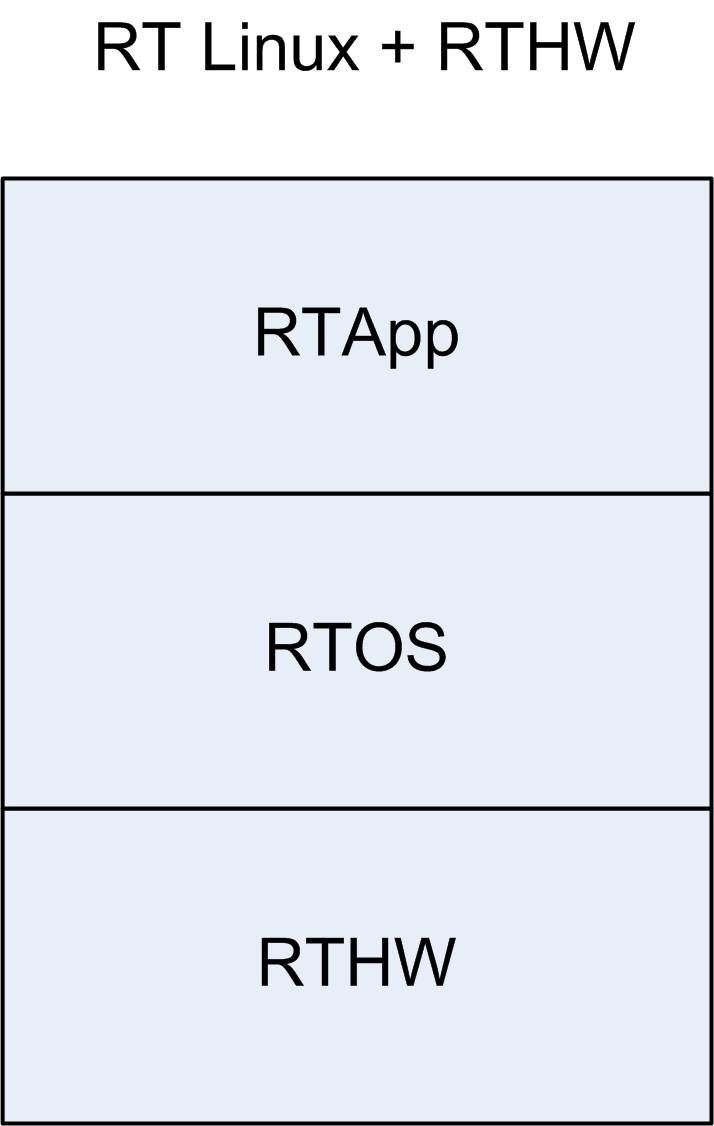
\includegraphics[width=0.25\hsize]{rtsystema}}
   \hspace{0.02\hsize}
   \subfigure[]{\label{rtsystemb}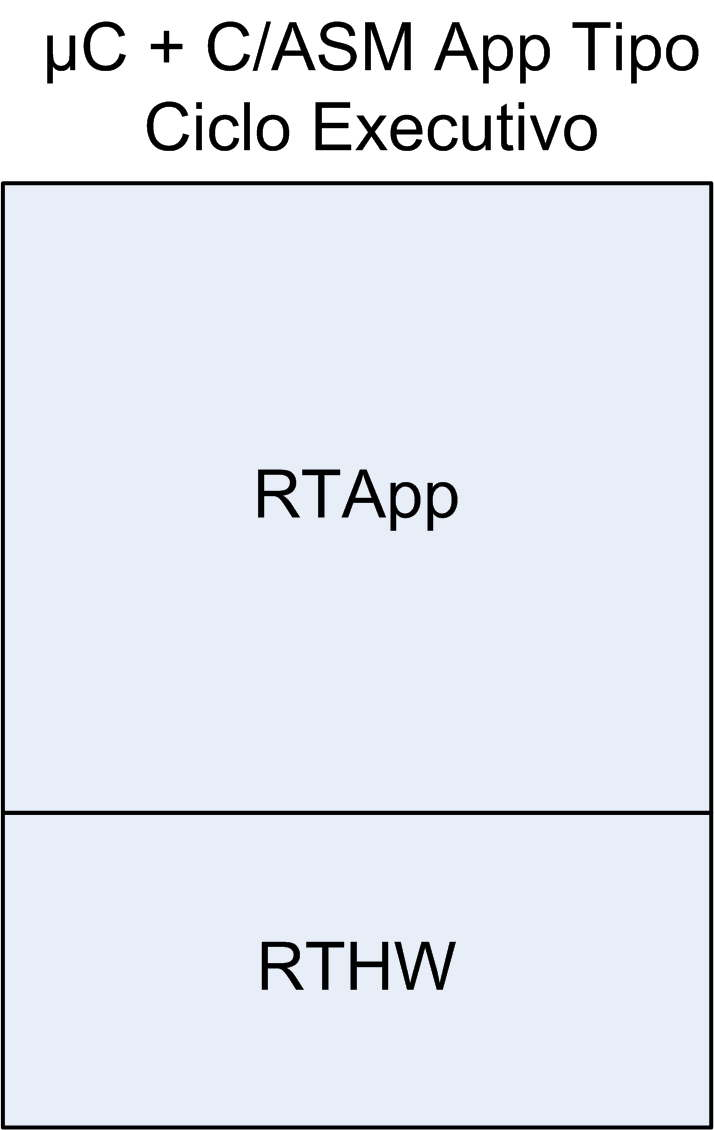
\includegraphics[width=0.25\hsize]{rtsystemb}}
   \hspace{0.05\hsize}
   \caption{implementa��o em camadas de um sistema de tempo real.}
   \label{rtsystem}
\end{figure}
A primeira � baseada em uma aplica��o de tempo real (RTApp), a qual implementa os requisitos funcionais do sistema, um sistema operacional de tempo real (neste exemplo, o RT Linux),  o qual faz o gerenciamento dos recursos e o escalonamento de tarefas, e um \emph{hardware} apropriado para tempo real (simbolizado aqui como RTHW). Na segunda implementa��o, n�o existe RTOS e a pr�pria aplica��o (RTApp - \emph{Real Time Application}) implementa o objetivo propriamente dito do sistema, al�m de promover o gerenciamento dos recursos. Este �ltimo � tamb�m conhecido como ciclo executivo, pois, as tarefas s�o listadas sequencialmente em um la�o.


	Algumas das t�cnicas de projeto que os engenheiros usam para atender a estes requisitos de tempo e confiabilidade s�o redund�ncia, paralelismo real, algoritmos de escalonamento de tempo real e simplifica��o do sistema  \cite{RTProgLang}. Obviamente, isso pode envolver uma penaliza��o associada ao tempo de desenvolvimento, custo final e desempenho m�dio do sistema. Portanto, estas t�cnicas de projeto devem ser aplicadas com parcim�nia e especificidade para cada sistema.
\section{Determinismo e an�lise temporal}
	Os sistemas computacionais modernos usualmente t�m recursos dispon�veis, tais como: Acesso Direto � Mem�ria (DMA), \emph{cache} de mem�ria, \emph{pipeline}, \emph {branch prediction}, gerenciador de mem�ria, escalonador de processos, fun��es de entrada/sa�da e comunica��o inter-processos. Em um sistema comum (que n�o � de tempo real), estes recursos d�o ao usu�rio do sistema, ou ao ambiente que o circunda, a impress�o de que v�rias tarefas est�o acontecendo em paralelo e prezam por um desempenho m�dio. Entretanto, um sistema de tempo real precisa restringir o n�o-determinismo encontrado em sistemas concorrentes comuns. Neste sentido, procura-se simplificar o sistema de forma a facilitar a an�lise do mesmo. No entanto, � importante entender que algumas penalidades podem ocorrer por simplificar bastante o sistema. Primeiro, a an�lise pode ser extremamente pessimista e pode n�o reproduzir a real situa��o ocorrida na maior parte do tempo. Logo, pode-se gerar um outro problema cl�ssico de sistemas de tempo real, a introdu��o de \emph{jitter}, que � a diferen�a entre os tempos de execu��o no melhor caso e no pior caso. A segunda penalidade, a rigidez imposta ao sistema, significando que uma pequena modifica��o no sistema como, por exemplo, inserir um novo processo, pode acarretar uma completa re-an�lise temporal e mesmo em outras modifica��es no sistema.

	Em sistemas de tempo real as tarefas s�o executadas em tempo determinado, visando a opera��o normal destes sistemas. Assim, instantaneamente, cada tarefa est� associada a um marco no tempo, ou seja, a um \emph{deadline}. A partir deste, se o sistema n�o responder ao est�mulo da entrada, este pode sofrer uma transi��o para um estado indesej�vel. Em sistemas de tempo real do tipo \emph{hard}, um \emph{deadline} perdido pode levar a uma falha catastr�fica. J� em sistemas de tempo real do tipo \emph{soft}, a perda de um \emph{deadline} pode levar o sistema a funcionar fora de sua especifica��o. A garantia de que \emph{deadlines} ser�o cumpridos baseia-se na an�lise temporal da execu��o do sistema no pior caso. Nesta an�lise, calcula-se o tempo exato de execu��o do pior caso ou WCET (\emph{Worst Case Execution Time}) \cite{jop:wcet:spe}. Este c�lculo � realizado baseado no modelo temporal do \emph{hardware}, no algoritmo de escalonamento do sistema operacional e na aplica��o, podendo ser realizado manualmente, mas preferencialmente com o aux�lio de uma ferramenta de \emph{software}.

	Para se obter o WCET de forma anal�tica, � necess�rio se obter o comportamento temporal do processador em quest�o. No entanto, o modelo temporal detalhado dos processadores modernos � n�o trivial devido �s caracter�sticas, tais como \emph{caches}, \emph{pipelines} e \emph{branch prediction}. Estas caracter�sticas ajudam a reduzir o tempo m�dio de execu��o, mas podem ser dif�ceis de prever seus impactos no WCET. Al�m disso, muitas informa��es necess�rias podem ser propriet�rias e dif�ceis de serem obtidas, mesmo sobre NDA (\emph{Non-Disclosure Agreement}).

\section{Hardware de tempo real}
	O hardware de um processador moderno cont�m estruturas paralelas que o auxiliam em suas tarefas, tais como DMA (\emph{Direct Memory Access}), \emph{cache} de mem�ria, \emph{pipeline} e \emph {branch prediction}. Estas estruturas introduzem maior complexidade em seu modelo temporal.

	A \emph{cache} de mem�ria de um processador � um recurso que aumenta o desempenho m�dio de um sistema computacional, mas por outro lado, introduz uma grande imprevisibilidade de tempo de execu��o de uma tarefa. Isto porqu� o algoritmo de \emph{cache} pode acertar ou errar quais s�o as pr�ximas instru��es ou dados a serem utilizados. Para solucionar este problema, pode-se desabilitar a \emph{cache} ou fazer uso de um processador mais simples, sem este recurso. Em um primeiro instante, esta abordagem pode parecer como uma fuga ao problema, por falta de compet�ncia para se fazer a an�lise complexa do sistema com o uso de \emph{cache}. No entanto, essa abordagem pode ser justificada pela seguinte m�xima na comunidade de projetistas desses sistemas: ``simplicidade contribui para confiabilidade". Neste caso, ou seja, em sistemas de tempo real do tipo \emph{hard}, deseja-se a solu��o mais segura, ainda que menos elegante.

    Al�m da complexidade do modelo temporal, de uma maneira geral, esses modelos ou mesmo as informa��es necess�rias para mont�-los, n�o est�o facilmente dispon�veis, devendo o interessado entrar em acordo legal (NDA - \emph{Non Disclosure Agreement}) com o fornecedor do circuito integrado para tentar obt�-los.
\section{Escalonamento de processos em sis\-te\-mas de tem\-po re\-al}
\subsection{Ciclo de execu��o}
	Para o problema de escalonamento de processos, a solu��o simplificada � o uso de execu��o c�clica, cont�nua e repetida de uma sequ�ncia de tarefas. Cada tarefa ocupa uma pequena parte do tempo como est� mostrado na Figura \ref{cyclicexecutive}, chamada de \emph{minor frame} (ou \emph{frame} secund�rio) e a soma de todas as tarefas ocupa um tempo conhecido por \emph{major frame} ou \emph{frame} principal \cite{RTProgLang}.	

\begin{figure}[!htb]
\centering

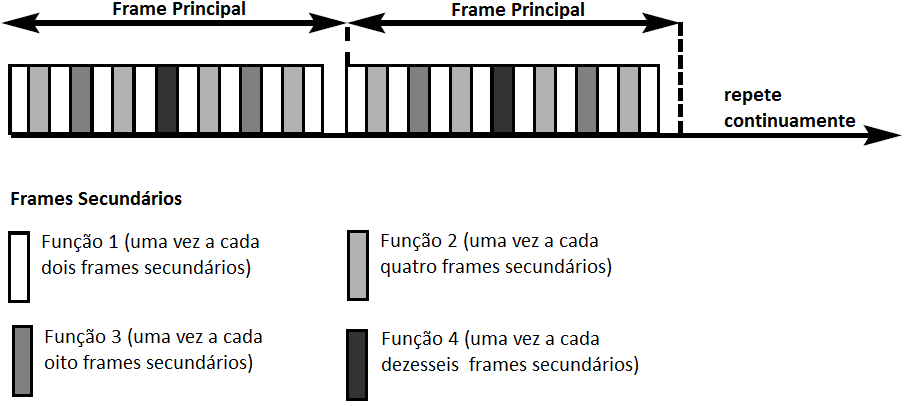
\includegraphics[width=4.5in]{cicloexecutivo}

\caption{ciclo executivo, adaptado de \cite{TimeSys}.}
\label {cyclicexecutive}

\end{figure}


\subsection{Prioridade fixa / peri�dicos}
	A maioria dos sistemas operacionais de tempo real usa um escalonador de prioridade fixa preemptivo (ou FPS - \emph{Fixed Priority Scheduling}). Nesse caso, o conjunto de processos � fixo, e a cada um destes � atribu�da uma prioridade tamb�m fixa. Preemptivo significa que, sempre que um processo de maior prioridade est� pronto para ser executado, e um processo de menor prioridade estiver em execu��o, este �ltimo � imediatamente interrompido para que o processo de maior prioridade seja executado. Este esquema � preferido por permitir uma rea��o mais r�pida dos processos de alta prioridade.  Esta forma de atribuir prioridades � �tima no sentido de que, se um conjunto de processos $P$ � escalon�vel, ent�o a atribui��o de prioridades monot�nicas em fun��o da frequ�ncia de execu��o � uma das solu��es para o problema de escalonamento do conjunto de processos $P$, sem perdas de \emph{deadlines} \cite{JopHandbook, RTProgLang}.

	Considere um conjunto de $N$ processos $P$. Sejam $T_i$ e $C_i$, o per�odo de execu��o e tempo m�ximo de execu��o do processo $i$, respectivamente. O uso computacional do sistema � calculado da seguinte forma:

\begin{equation}\label{usocomp}
U=\sum_{i=1}^n \frac{C_i}{T_i}
\end {equation}

	Demonstra-se que se $U\leq N \cdot ( {2}^{\frac{1}{N}} - 1 )$ e se as prioridades dos processos forem atribu�das obedecendo � monotonicidade da frequ�ncia de execu��o ($\frac{1}{T_i}$) e com preemp��o, ent�o, o conjunto de processos $P$ � escalon�vel, e portanto todos os \emph{deadlines} s�o sempre obedecidos. Com o crescimento de $N$, a express�o converge assintoticamente para 0,63. Esta condi��o � suficiente, mas n�o necess�ria para que o conjunto de processos $P$ seja escalon�vel. A raz�o de n�o ser necess�ria � que, em muitos casos, � poss�vel ter um uso computacional maior e ainda assim, o sistema ser escalon�vel \cite{liulayland}.
\subsubsection{Problema da invers�o de prioridade e solu��o}

	Usando um algoritmo de prioridade fixa, depara-se com o problema de invers�o de prioridade, situa��o na qual um processo de alta prioridade � bloqueado por um processo de baixa prioridade que det�m um recurso compartilhado entre estes processos. A Figura \ref{priorityinversion} exemplifica esta situa��o.
\begin{figure}[!htb]
\centering

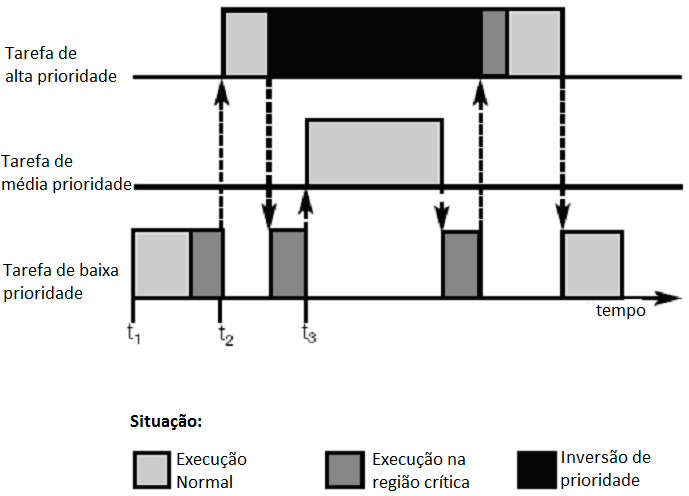
\includegraphics[width=4.0in]{priorityinversion}

\caption{invers�o de prioridades, adaptado de \cite{TimeSys}.}
\label{priorityinversion}

\end{figure}
Durante todo o per�odo em que a tarefa de maior prioridade (assinalada com a cor preta) est� esperando que o processo de menor prioridade saia da regi�o cr�tica, o que � razo�vel. Por�m n�o � aceit�vel que, nesta condi��o, o processo de prioridade intermedi�ria interrompa a execu��o do processo de menor prioridade, pois, por transfer�ncia, o processo de maior prioridade est� esperando por este \cite{TimeSys}.


	Uma solu��o para esse problema � o uso de um protocolo de sincroniza��o, como por exemplo o protocolo de heran�a de prioridades. Usualmente, a implementa��o deste protocolo est� associada �s modifica��es nas fun��es de acesso � regi�o cr�tica. A RTSJ (\emph{Real Time Specification for Java}), por exemplo, prev� uma solu��o baseada em heran�a de prioridades para resolver o problema de invers�o de prioridades.
\subsection{Algoritmo do \emph{deadline} mais pr�ximo}
	Neste algoritmo, tamb�m conhecido como EDF (\emph{Early Deadline First}), sempre � escalonada para execu��o a tarefa que est� com seu \emph{deadline} mais pr�ximo. Liu e Layland demonstraram que, se o uso computacional $U$ de um conjunto de tarefas for menor do que 1, ent�o este conjunto � escalon�vel seguindo este algoritmo e, portanto, os \emph{deadlines} ser�o sempre cumpridos \cite{liulayland}.

	Apesar desse algoritmo permitir um uso computacional efetivo do sistema (100\%), as prioridades s�o calculadas dinamicamente, e isto dificulta a implementa��o do escalonador. Al�m disso, em situa��es n�o previstas de carga m�xima, o determinismo do sistema � menor do que se este fosse baseado em prioridades fixas.
\subsection{Escalonamento de tarefas aperi�dicas}
	As tarefas aperi�dicas s�o disparadas por eventos tais como requisi��es do operador, mensagens de emerg�ncia, notifica��o de alcance de limiar, um bot�o pressionado ou o movimento de um mouse, dentre outros exemplos.

	Em particular, uma abordagem para lidar com eventos aperi�dicos em sistemas de tempo real, � atrav�s do uso de um servidor aperi�dico. Este servidor deposita ``passes'', os quais s�o revalidados depois de um certo per�odo ap�s terem sido usados. Quando um evento aperi�dico ocorre, este verifica se existem ``passes'' dispon�veis no servidor. Se existirem, o sistema imediatamente processa o evento, e ent�o escalona a cria��o de outro ``passe'', baseado nas pol�ticas de cria��o de ``passes''. Um servidor aperi�dico imp�e previsibilidade em tarefas aperi�dicas e, portanto, torna-as adequadas para serem escalonadas, utilizando os algoritmos de EDF ou FPS explicados nas se��es anteriores.

    Ap�s mostrar e discutir nesta se��o os principais algoritmos utilizados, para escalonamento de processos em sistemas de tempo real, na pr�xima se��o discorre-se, sucintamente, sobre o gerenciamento de mem�ria em sistemas de tempo real.

\section{Gerenciamento de mem�ria}
	Em sistemas de tempo real, uma abordagem bastante adotada para o gerenciamento de mem�ria � criar todos os processos e alocar mem�ria estaticamente, na fase de inicializa��o do sistema. Portanto, antes da opera��o propriamente dita do sistema, toda a mem�ria a ser utilizada durante todo o tempo de miss�o deve estar previamente alocada. A penaliza��o � que o total de mem�ria necess�rio para o sistema � significativamente maior do que no caso de aloca��o din�mica de mem�ria, no qual a aloca��o � feita em tempo de execu��o e desalocada sempre que esta regi�o n�o for mais necess�ria.	
\section{Toler�ncia a falhas}
	Uma falha pode causar um erro e este por sua vez, um defeito conforme mostrado na Figura \ref{falhaerrodefeito}. Idealmente, persegue-se detectar, confinar e corrigir a falha antes que esta cause um erro. Por isso, a falha � objeto de estudo prim�rio de sistemas tolerantes a falhas.

\begin{figure}[!htb]
\centering

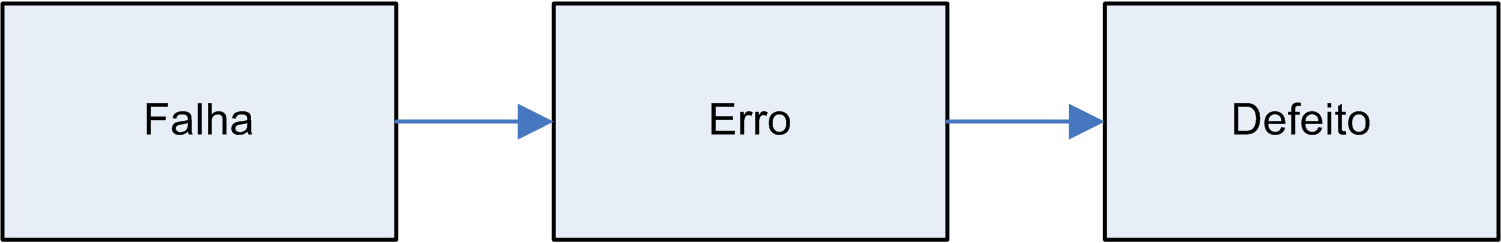
\includegraphics[width=4.5in]{falhaerrodefeito}

\caption{sequ�ncia de falha, erro e defeito, adaptado de \cite{helanothesis}.}
\label{falhaerrodefeito}

\end{figure}



	As falhas podem ser classificadas como antecipadas e n�o antecipadas. Uma falha de projeto, por exemplo, � uma falha n�o antecipada, pois certamente o projeto n�o foi feito errado de prop�sito \cite{anderson81}.

	Ap�s detectar uma falha, o sistema deve imediatamente tentar identificar a extens�o dos poss�veis erros e danos j� causados por esta falha. Ap�s isto, medidas devem ser tomadas para que o erro n�o se propague, ou seja, para que outras partes do sistema n�o operem baseados em dados err�neos fornecidos pelas partes do sistema que foram afetados pela falha. Essa fase � conhecida como confinamento da falha.

	O processo de corre��o de falhas envolve, quando poss�vel, recuperar todos os erros causados por esta. Na impossibilidade de recuperar o sistema, este pode tentar operar de forma degradada. Suponha por exemplo, um sistema de telefonia. Uma opera��o em modo degradado poderia permitir, ou garantir apenas a realiza��o de chamadas de emerg�ncia.

	Em �ltima hip�tese, o sistema deve tentar entrar em modo de falha seguro. No modo de falha seguro, o sistema, ciente de que est� defeituoso, n�o continua a operar, pois, suas execu��es podem causar danos maiores ainda. 	Assim, deve-se prever na arquitetura do sistema, recursos adicionais (de \emph{hardware} e de \emph {software}) que suportem procedimentos para toler�ncia a falhas. A arquitetura de um sistema tolerante a falhas � projetada de forma a fornecer ao sistema recursos extras, de \emph{hardware} e de \emph{software}, para realizar as a��es j� descritas de detec��o e corre��o de falhas.

Uma das principais arquiteturas de \emph{hardware} para sistemas tolerantes a falha, � a arquitetura de redund�ncia modular tripla ou TMR (\emph{Triple Modular Redundancy}). Na redund�ncia modular tripla, o sistema computacional � replicado tr�s vezes e um votador � adicionado. Os tr�s sistemas computacionais funcionam em paralelo (\emph{hot stand-by}) e o resultado considerado correto � aquele apontado por no m�nimo dois m�dulos. O votador, que � um ponto de falha comum, por ser um sistema muito menos complexo que uma das r�plicas do sistema computacional, usualmente tem uma probabilidade de falha pequena comparada aos m�dulos computacionais. Ainda assim, � poss�vel replicar tamb�m o votador. Note que em um sistema TMR a falha somente � detectada ap�s a mesma ter causado um erro computacional, por�m antes que o erro se torne um defeito.	
\subsection{C�lculo de confiabilidade}
	O c�lculo da confiabilidade de um sistema � o ponto de partida para a decis�o de se adicionar t�cnicas de toler�ncia � falhas. Pela compara��o entre a confiabilidade esperada e a confiabilidade atual do sistema, o projetista pode tomar decis�es.

	Para sistemas simples, sem redund�ncia, estes c�lculos s�o triviais e se baseiam em probabilidade simples. Por exemplo, a confiabilidade de um sistema s�rie � calculada multiplicando-se a confiabilidade de cada um dos componentes do sistema, dada por \cite{helanothesis}
\begin{equation}\label{confiabilidadeserie}
R_s=\prod_{i=1}^n {R_i},
\end {equation}
sendo $R_s$ a confiabilidade do sistema s�rie e $R_i$ a confiabilidade do componente $i$.

	Em sistemas com redund�ncia, os m�dulos replicados podem entrar em funcionamento desde o in�cio da fase de miss�o (\emph{hot standby}), ou dinamicamente de acordo com as necessidades do sistema (\emph{cold standby}). Baseado em um diagrama de estados dos m�dulos do sistema, o c�lculo da confiabilidade pode ser feito baseado em cadeias de Markov \cite{shoomanbook}.
\subsection{Detec��o e corre��o de erros em uma sequ�ncia de dados}
	Sistemas com corre��o de erro sem reenvio de informa��es s�o tamb�m conhecidos como FEC (\emph{Forward Error Correction}). Nesse caso, o c�digo de corre��o de erros ou ECC (\emph{Error Correction Code}), que s�o dados redundantes, s�o enviados em um �nico pacote ou bloco juntamente com os dados originais.
\subsubsection{Checagem por redund�ncia c�clica}
	CRC (\emph{Cyclic Redundancy Check}) � um algoritmo utilizado para detec��o de erros durante transmiss�o de dados. Para detectar tais erros, o CRC utiliza-se de um complexo polin�mio para gerar um n�mero baseado no dado a ser transmitido. O c�lculo do CRC � feito pelo dispositivo que ir� enviar esses dados (transmissor) e, ap�s a transmiss�o, pelo dispositivo que os recebeu (receptor). Caso os dois dispositivos tenham obtido os mesmos valores de CRC, a transmiss�o ocorreu livre de falhas. Existem v�rias formas de calcular o CRC, diferem-se pelo polin�mio adotado e pela forma de entrada dos dados, paralelamente ou serialmente \cite{crc1,crc2}.
\subsubsection{Algoritmo de Hamming}
	O algoritmo de Hamming � capaz de corrigir e detectar erros em uma sequ�ncia de \emph{bits} e � relativamente simples e de f�cil implementa��o, tanto em \emph{software}, como em \emph{hardware}. A limita��o do algoritmo de Hamming est� nas suas habilidades para realizar corre��es. � poss�vel detectar e corrigir um erro em um �nico \emph{bit}. O algoritmo de Hamming � usualmente especificado pelo tamanho do bloco em \emph{bits} e o n�mero de \emph{bits} desse bloco que se refere ao dado original. Por exemplo, Hamming (255, 247), refere-se a uma codifica��o de Hamming com blocos de tamanho 255 \emph{bits}, sendo 8 \emph{bits} redundantes. De uma maneira geral, definem-se \cite{shoomanbook}
	\begin{equation}\label{hamdef}
     \left\{%
\begin{array}{ll}
    n~\mbox{como o n�mero de \emph{bits} de redund�ncia}; e\\
    (2^n - 1)~\mbox{o tamanho total do bloco, incluindo n \emph{bits} de redund�ncia}. \\
\end{array}%
\right.
\end{equation}
Assim, tem-se que o n�mero de \emph{bits} de dados em um bloco � $(2^n-1) -n$.

	Os \emph{bits} redundantes s�o calculados por uma s�rie de opera��es ``ou exclusivo" (\texttt{xor}) sobre os \emph{bits} de entrada, e ent�o montados em um bloco contendo os \emph{bits} de entrada e os \emph{bits} de Hamming, com a ordem de sequenciamento desses \emph{bits} ditada pelo algoritmo.

	Para verificar se ocorreu um erro, os valores esperados dos \emph{bits} redundantes s�o calculados (com base nos \emph{bits} de dados recebidos) e comparados com os \emph{bits} de Hamming recebidos. Caso haja qualquer diverg�ncia entre \emph{bits} calculados e recebidos, significa que um erro foi detectado.

	Para recuperar o erro, o algoritmo, atrav�s de opera��es ou exclusivo descobre qual a posi��o do bloco cont�m um bit errado. Com a posi��o dada, para realizar a corre��o basta inverter o \emph{bit} na posi��o apontada pelo algoritmo. � importante ressaltar que � poss�vel detectar e corrigir um erro ocorrido em apenas um bit.

	Modificando-se o algoritmo original de Hamming pelo acr�scimo de mais um \emph{bit} de redund�ncia no tamanho do bloco, � poss�vel detectar at� dois \emph{bits} errados. O \emph{bit} adicional � um \emph{bit} de paridade do restante do bloco. O processo de corre��o � id�ntico ao algoritmo original e corrige tamb�m apenas um \emph{bit}.
\subsubsection{Outros algoritmos de corre��o de erros}
	Existem algoritmos com uma corre��o de erros mais robusta, capazes de corrigir v�rios \emph{bits} errados, como Reed Solomon e BCH (Bose-Chaudhuri-Hocqueenghem). Estes algoritmos s�o prefer�veis para corre��es de erros em canais ruidosos ou em mem�rias \emph{flash} do tipo \texttt{nand} com c�lulas multicamada (\emph {Multi Layer Cell}), em que a probabilidade de erros em v�rios \emph{bits} � alta. Reed Solomon � um caso particular de BCH e tem menor efici�ncia. Apesar de serem mais eficientes, esses algoritmos s�o muito mais complexos do que Hamming e, portanto, consomem muito mais c�lulas l�gicas ou ciclos de rel�gio (\emph{clock}).

\section{Java para sistemas de tempo real}
\subsection{Sistemas atuais}
	A linguagem de programa��o C � a principal linguagem utilizada atualmente para desenvolvimento de \emph{software} para sistemas embarcados, tanto para o sistema operacional quanto para a aplica��o. Fun��es de suporte a tempo real, gerenciamento de mem�ria e comunica��o inter-processos s�o usualmente desempenhadas por um sistema operacional de tempo real e s�o acess�veis pela aplica��o atrav�s de Chamadas de Sistema \cite{TanenbaumModernOS} e de uma API (\emph{Application Progam Interface}).
\subsection{Vantagens da linguagem Java}
	As principais caracter�sticas da linguagem Java s�o: ser fortemente tipada; ter extensa checagem em tempo de execu��o e compila��o; n�o ter ponteiros; possuir monitores; ter meios de comunica��o inter-processos; ser \emph{multi-thread}; ter checagem e tratamento de exce��es.
	Para sistemas operando sobre uma m�quina virtual Java, essas fun��es s�o desempenhadas pela m�quina virtual e est�o dispon�veis para serem usadas pela aplica��o, atrav�s de estruturas pr�prias da linguagem de programa��o Java e n�o atrav�s de chamadas de sistema. Essa abordagem tamb�m � utilizada por outras linguagens de programa��o cl�ssicas de sistemas de tempo real, como Occam 2, Modula 2 e Ada \cite{RTProgLang}. Al�m disso, a linguagem Java n�o trabalha com ponteiros e tem uma extensa checagem de exce��es em tempo de compila��o e de execu��o, o que a torna menos propensa a erros do programador em rela��o � linguagem C. Portanto, a linguagem Java permite que o programador de sistemas embarcados use um n�vel de abstra��o maior, dando foco no desenvolvimento da aplica��o.
\subsection{Desvantagens da linguagem Java}
	Em sistemas embarcados, a M�quina Virtual Java pode ser executada no topo de um sistema operacional Linux, por exemplo. Vers�es recentes da JVM (\emph{Java Virtual Machine}) utilizam recursos como compila��o JIT (\emph{Just in Time}) para otimizar o desempenho dos sistemas. No entanto, essa solu��o n�o � interessante para sistemas embarcados, devido � restri��o de recursos do mesmo quando comparados a um computador pessoal. Uma outra desvantagem � a introdu��o de \emph{jitter} no tempo de execu��o das aplica��es, devido ao sistema de \emph{garbage collector} \cite{jop:tecs:nbgc,jop:rtsgc:rts}. Schoeberl analisou estas restri��es da linguagem Java e fez uma implementa��o eficiente em {hardware} de uma m�quina virtual Java com aplica��o em sistemas embarcados de tempo real \cite {JopHandbook}.
\subsection{Especifica��o Java para sistemas de tempo real}
	Existem, particularmente, dois tipos de sistema de tempo real que s�o bastante desenvolvidos em Java, e est�o, h� v�rios anos, aguardando por uma especifica��o e implementa��o de tempo real para Java: Sistemas Financeiros e Sistemas Embarcados. Apesar da requisi��o por uma especifica��o Java ser bem antiga (data de antes do ano 2000), que ali�s � a primeira JSR (\emph{Java Specification Request}), a RTSJ (\emph{Real Time Specification for Java}) ainda � um trabalho em andamento.

	Diferentemente de outras linguagens de programa��o, quando se fala de Java, n�o � simplesmente da sem�ntica e das fun��es dispon�veis em uma linguagem de programa��o, mas, al�m disso, referm-se a um ambiente de execu��o, a m�quina virtual Java. Essa m�quina virtual Java pode interfacear diretamente com o \emph{hardware} ou atrav�s de um sistema operacional. Em um ambiente de desenvolvimento para tempo real em Java, todos os elementos supracitados devem ser de tempo real, ou seja, a linguagem Java, JVM, RTOS e o \emph{hardware}. Como as carac\-te\-r�s\-ti\-cas do \emph{hardware} e dos sistemas operacionais de tempo real foram discutidas nas se��es anteriores, n�s iremos nos deter em JVM e na linguagem de programa��o Java.

	Dois pontos de vista distintos podem ser definidos em rela��o � especifica��o RTSJ: o do projetista de m�quinas virtuais Java de tempo real e o do programador de aplica��es Java de tempo real. Para o primeiro, as caracter�sticas de previsibilidade e confiabilidade precisam ser adicionadas � JVM. Nessa dire��o, os principais problemas est�o relacionados ao gerenciamento de mem�ria (\emph{Garbage Collector}); escalonamento de \emph{threads}; sincroniza��o de threads; gerenciamento de tempo com alta resolu��o; tempo m�ximo de repostas a interrup��es.

De acordo com a RTSJ, o \emph{garbage collector} n�o deve atuar na �rea de mem�ria utilizada pelas \emph{threads} de tempo real do tipo \emph{noheap}, pois, a mem�ria alocada para essas \emph{threads} � completamente est�tica e reside na �rea denominada \emph{immortal}. Esta � uma regi�o reservada para aloca��es est�ticas, ou seja, na qual o garbage collector n�o atua. Notadamente, a solu��o adotada para a concorr�ncia por recursos entre \emph{garbage collector} e \emph{noheap threads} foi eliminar a regi�o cr�tica.	Ainda do ponto de vista do projetista de m�quinas virtuais, para projetar uma m�quina virtual Java compat�vel com o padr�o RTSJ, o algoritmo de FPS deve ser utilizado para escalonamento de processos, al�m da ado��o de uma solu��o para o problema de invers�o de prioridades.

Do ponto de vista do segundo, o programador de aplica��es, este necessita de uma API e sem�ntica adequadas para controlar o comportamento temporal do sistema. Neste sentido, A RTSJ define um conjunto de classes e m�todos para facilitar a implementa��o de sistemas de tempo real. Os primeiros passos s�o instalar na JVM  a extens�o RTS e renomear todas as ins\-tan\-cia\-��es de \texttt{java.lang.Thread} para \texttt{javax.realtime.Realtime\-Thre\-ad}. Por�m, como n�o existe uma solu��o �nica para programa��o de sistemas de tempo real, � necess�rio a coopera��o do programador de aplica��es para o correto desenvolvimento do sistema.


\subsection{Especifica��o Java para sistemas cr�ticos de tempo real}
	Por consumir muitos recursos do sistema, a RTSJ n�o � adequada para implementa��o de uma JVM para uso em sistemas embarcados \cite{JopHandbook}. Schoeberl implementou uma m�quina virtual Java para sistemas embarcados que atende a um subconjunto da RTSJ.

	N�o obstante, a JSR de n�mero 302 refere-se � extens�o do padr�o Java 2 Micro Edition (J2ME) para aplica��o em sistemas com n�vel de confiabilidade cr�tico (\emph{hard real time}). A especifica��o baseia-se na RTSJ e cont�m as caracter�sticas m�nimas necess�rias para um sistema ser certificado como DO-178B compat�vel \cite{jop:scjava}. Esta especifica��o foi nomeada SCJ (\emph{Safety Critical Java}) e encontra-se em fase de desenvolvimento \cite{jsr302}.

	Conforme pode ser visto na Figura \ref{scj}, tr�s fases s�o claramente distingu�veis no fluxo de execu��o de um sistema baseado em SCJ: inicializa��o, miss�o e recupera��o. A fase de inicializa��o n�o � de tempo real. Nesta fase, todos os objetos s�o instanciados e assim permanecem por toda a fase de miss�o, pois n�o h� \emph{garbage collector} na SCJ. Na fase de miss�o, que � de tempo real,  o sistema deve realizar sua fun��o propriamente dita, e assegurar os requisitos de tempo real da miss�o. Na ocorr�ncia de uma falha que n�o possa ser tratada pelos mecanismos de toler�ncia a falhas, sem comprometer a funcionalidade do sistema, o mesmo � levado � fase de recupera��o. Nesta fase, os danos s�o avaliados, a falha � confinada, e dependendo da gravidade do problema, o sistema pode entrar em modo de falha segura ou recuperar a aplica��o, e retornar � fase de inicializa��o.


\begin{figure}[!htb]
\centering

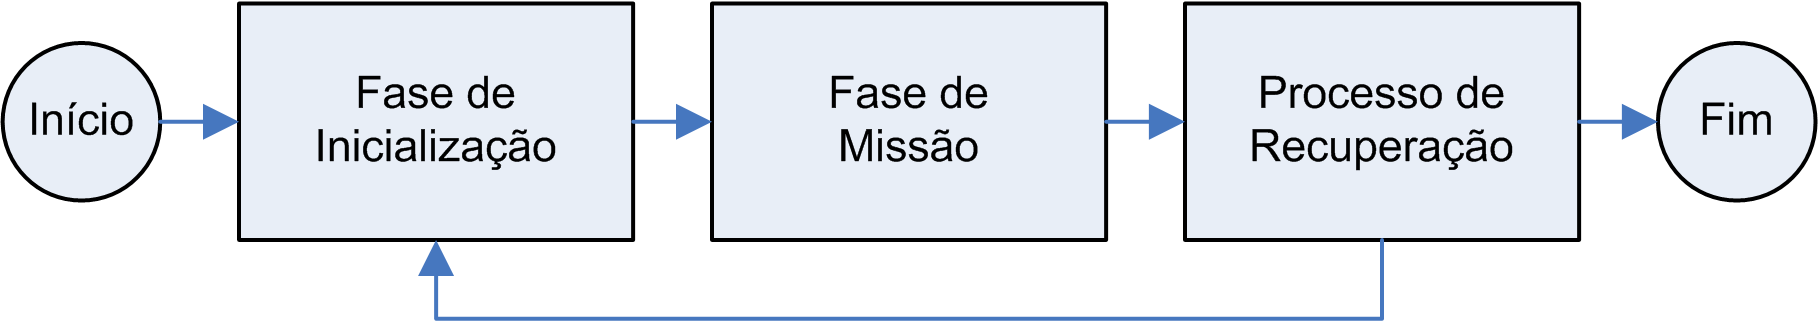
\includegraphics[width=4.5in]{scj}

\caption{fases de execu��o de uma aplica��o com modelo da especifica��o SCJ, adaptado de \cite{jop:scjava}.}
\label{scj}

\end{figure}


\section{Conclus�o}
	Um processador ideal para sistemas de tempo real deve ter um modelo temporal previs�vel e de f�cil an�lise, ao mesmo tempo, deve dispor dos recursos dos processadores modernos para que tenha um bom desempenho m�dio.

	Deve-se investir para melhorar a confiabilidade de um sistema tanto maior a probabilidade da ocorr�ncia de uma falha e mais custoso seu impacto.  Para sistemas de tempo real do tipo \emph{hard}, toda e qualquer caracter�stica que possa melhorar a confiabilidade do sistema deve ser considerada, ainda que outras vari�veis sejam penalizadas. Os demais sistemas de tempo real (que n�o envolvem riscos de vidas humanas) s�o do tipo \emph{soft}, como por exemplo um sistema de recep��o de multim�dia para entretenimento.	
 %cap 2

\chapter{Projeto de Circuitos Integrados L�gicos Digitais}
\label{Chapter:PCILD}

\PARstartOne{O}s equipamentos de tecnologia da informa��o e comunica��o est�o presentes no cotidiano do homem, seja quando utiliza um celular para se comunicar ou um \emph{laptop} para ler os \emph{emails}, dentre outros exemplos existentes. Os dispositivos semicondutores, tais como transistores, diodos e circuitos integrados s�o itens necess�rios para cons\-tru\-��o dos equipamentos eletr�nicos. Destes itens, os circuitos integrados merecem aten��o especial por terem embutido, em um �nico chip, in�meras fun��es e dispositivos eletr�nicos.

\section{Introdu��o}
	O projeto de um circuito integrado tem elevado custo de desenvolvimento e de prototipa��o. A decis�o por iniciar o projeto de um novo circuito integrado deve passar por uma an�lise detalhada de viabilidade t�cnica e mercadol�gica. Do ponto de vista t�cnico, esta decis�o est� associada aos requisitos da aplica��o, tais como desempenho e consumo. Ao se comparar na ordem decrescente de consumo e de aumento de desempenho, conforme mostra a Figura \ref{asicfit}, tem-se processadores de uso geral, processadores de uso espec�fico, FPGAs (\emph{Field-Programmable Gate Arrays}), CPLDs (\emph{Complex Programmable Logic Device}) e ASICs (\emph{Application-Specific Integrated Circuit}). Os ASICs apresentam o menor consumo e o maior desempenho, justamente por serem espec�ficos para uma determinada aplica��o \cite{ednasicfpga}.  	

\begin{figure}[!htb]
\centering

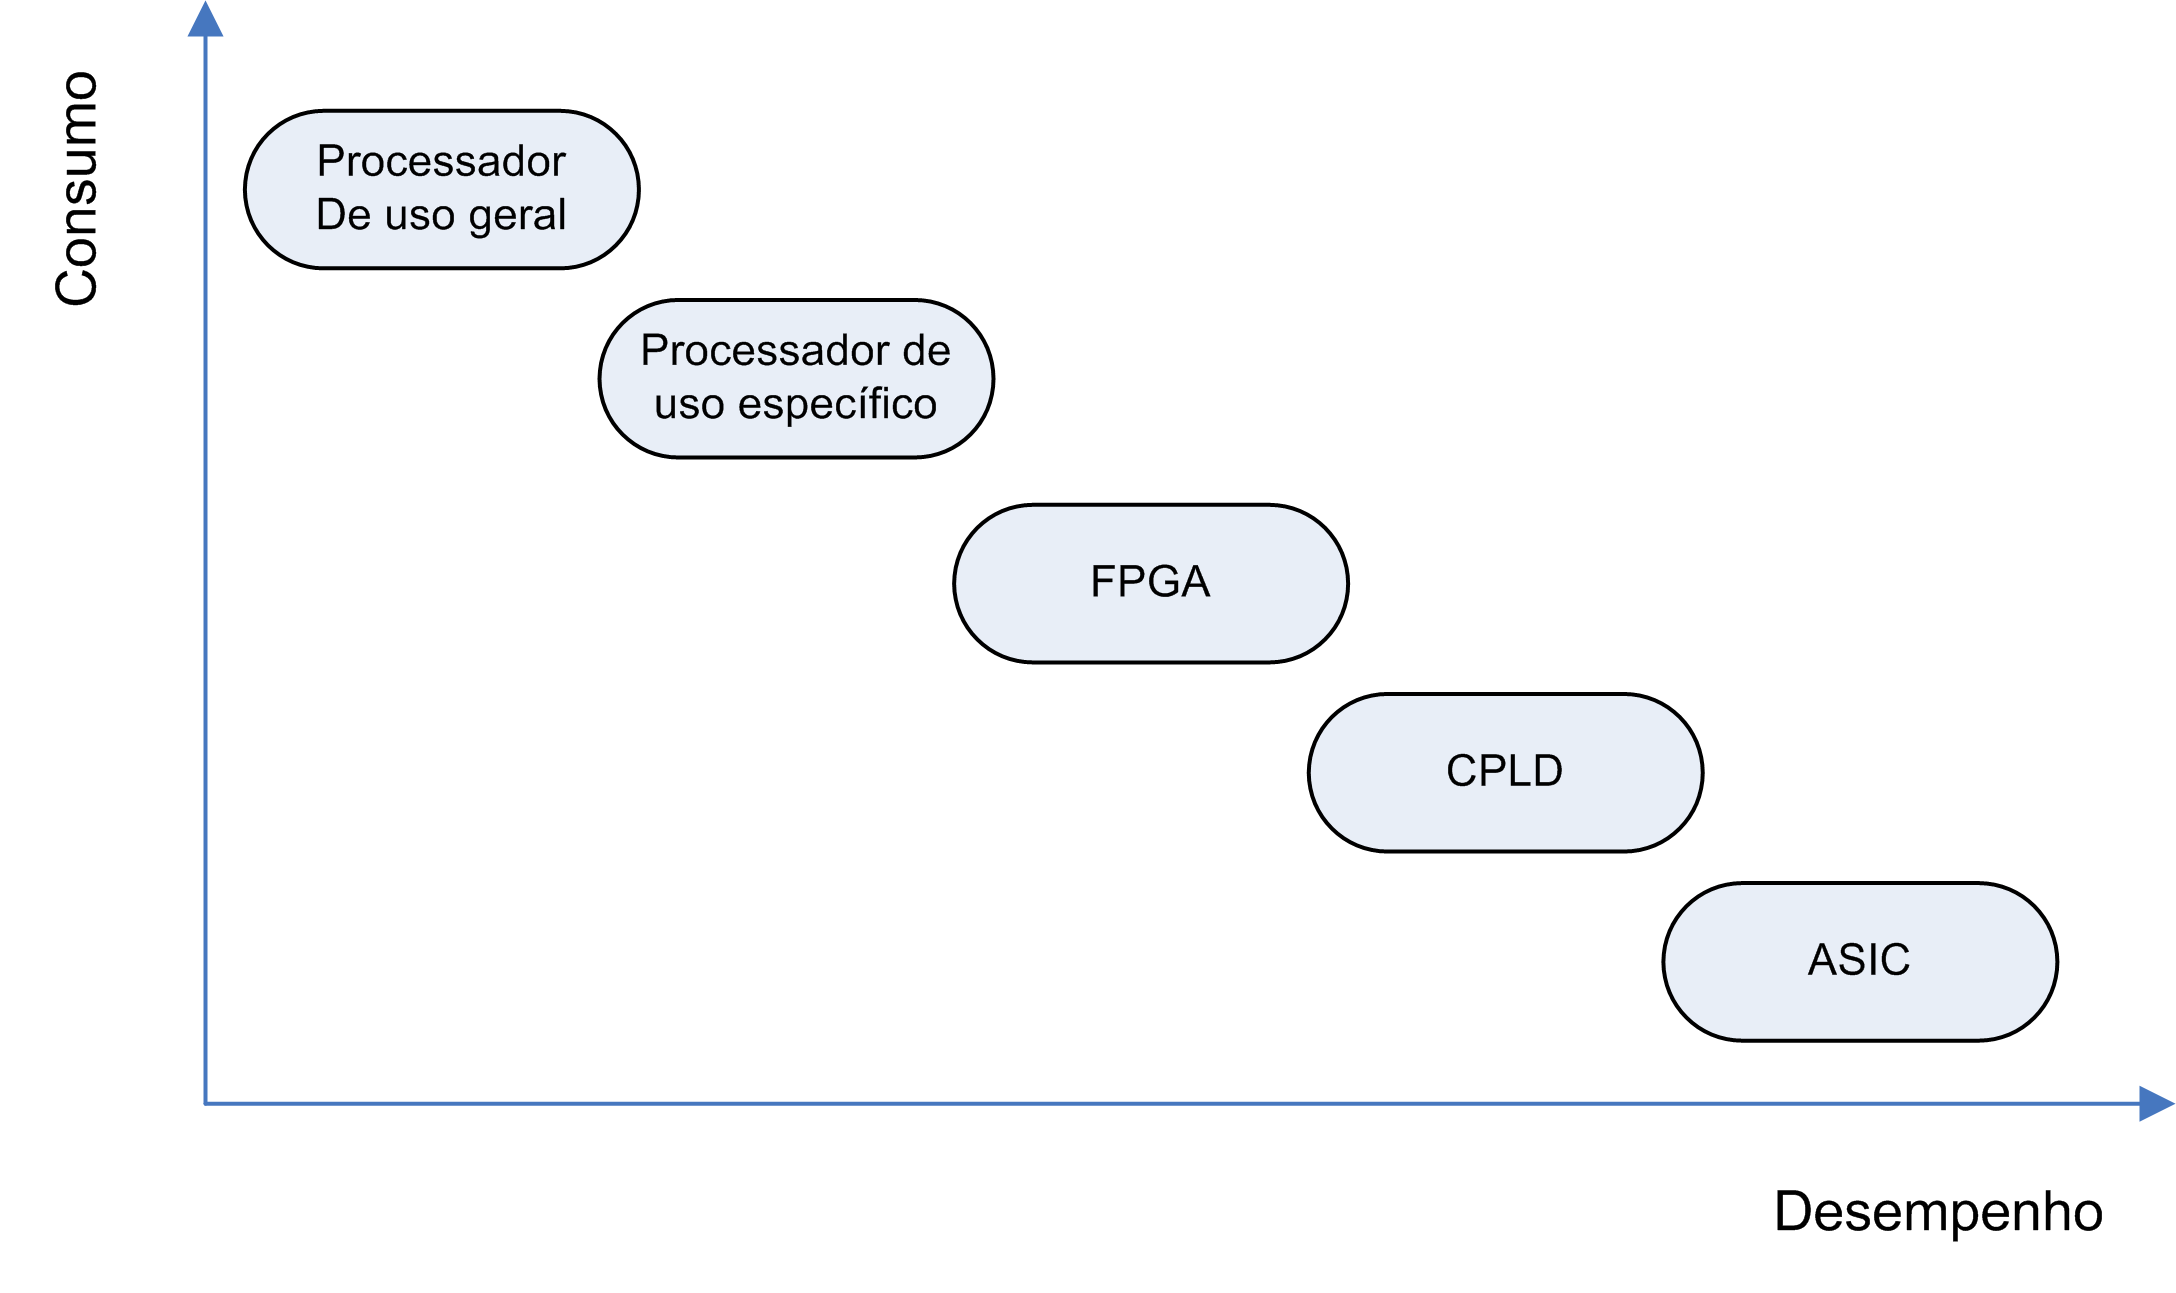
\includegraphics[width=4.5in]{asicfit}

\caption{consumo x desempenho das tecnologias para implementa��o de sistemas computacionais.}
\label{asicfit}

\end{figure}

	Do ponto de vista mercadol�gico, as principais vari�veis s�o: o volume de produ��o esperado, o tempo e o custo necess�rios para o desenvolvimento. O custo do desenvolvimento dever� ser dilu�do no volume de produ��o. Entretanto, se o tempo necess�rio para desenvolver o CI se sobrepuser muito � janela de oportunidade de vendas do produto, ent�o n�o valeria a pena iniciar seu projeto. Destacam-se dois exemplos que est�o nos extremos da rela��o volume de produ��o x custo de desenvolvimento.
	Considere, primeiramente, a decis�o que foi tomada para se projetar um CI para aplica��o em tocadores port�teis MP3. Do ponto de vista t�cnico, apenas um ASIC poderia atingir os requisitos de baixo consumo de um dispositivo dedicado a esta aplica��o. O volume de produ��o esperado seria muito grande e um CI para esta aplica��o n�o possui um custo de projeto t�o elevado. Logo, a decis�o por iniciar este CI � �bvia.
	Agora, considere um projeto de um equipamento para interfacear com redes �ticas e que precisa manipular um volume de dados da ordem de dezenas de Gigahertz. Este equipamento � utilizado por operadoras de telecomunica��es e tem uma produ��o esperada de poucas centenas de unidades e, al�m disso, tem um custo de produ��o da ordem de dezenas de milhares de d�lares. Neste caso, o projeto de um CI para manipular esse volume de dados � n�o trivial. Mesmo usando as tecnologias mais modernas de fabrica��o para viabilizar a opera��o nesta frequ�ncia, o leiaute dever� ser muito otimizado e, portanto completamente manual. Logo, teria o projeto um custo muito elevado e longo tempo de desenvolvimento. Neste sentido, a decis�o pelo uso de uma FPGA de alto desempenho e o n�o in�cio de um novo projeto de CI seria a mais acertada.
	Circuitos eletr�nicos podem ser projetados em v�rios n�veis e em ordem decrescente de complexidade, tem-se: sistema, m�dulo, porta l�gica, circuito e processo \cite{rabaey}, conforme mostra a Figura \ref{designlevel}.

\begin{figure}[!htb]
\centering

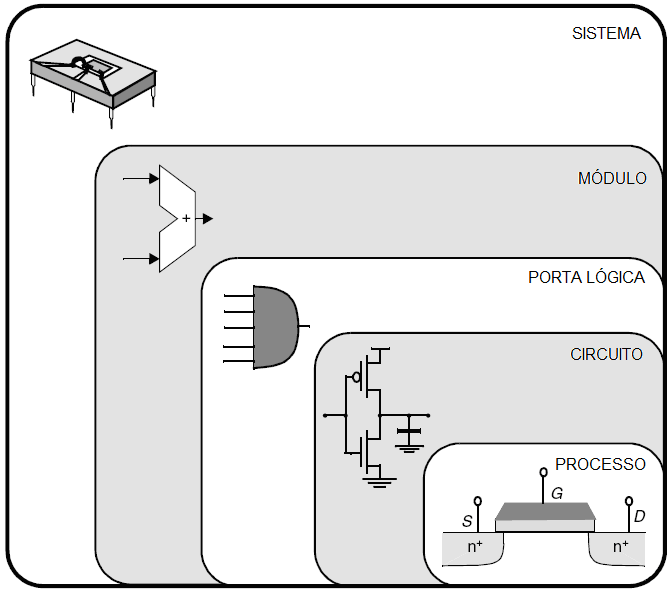
\includegraphics[width=3.0in]{designlevel}

\caption{n�veis de projeto de circuitos integrados, adaptado de \cite{rabaey}.}
\label{designlevel}

\end{figure}

\section{Estado da Arte e Desafios do \emph{Deep Sub Micron}}
	Em fun��o do volume de produ��o, os processos de fabrica��o para circuitos digitais (ou quase totalmente digitais) baseados em tecnologia CMOS (\emph{Complementary Metal-Oxide-Semiconductor}) dominaram o mercado, sobrepondo-se � tecnologia bipolar. Para circuitos digitais, a vantagem da tecnologia CMOS est� no consumo reduzido de energia.
	Por outro lado, os projetistas de circuitos anal�gicos, al�m de trabalharem com a tecnologia CMOS para desenvolverem seus circuitos, que � menos adequada do que a tecnologia bipolar, s�o obrigados a se adequar a uma redu��o cont�nua da tens�o de opera��o (de 12V da tecnologia bipolar para os 3.3V da tecnologia CMOS atual). A faixa de opera��o pequena de tens�o (0-3.3V) exige circuitos anal�gicos com uma melhor toler�ncia a ru�dos \cite{razavi}.

	Nos dias atuais, existem dispon�veis processos BICMOS (\emph{Bipolar Junction Transistors and CMOS}), os quais permitem ter no mesmo circuito integrado, circuitos desenvolvidos em tecnologia bipolar e circuitos desenvolvidos em tecnologia CMOS. O processador Pentium Pro, por exemplo, foi desenvolvido usando esta tecnologia.
	De acordo com o ITRS (\emph{The International Technology Roadmap for Semiconductors}), n�o existe uma alternativa com condi��es reais para substituir a tecnologia CMOS, pelo menos para os pr�ximos 15 anos, o que nos permite prever que a dimens�o da tecnologia de fabrica��o dos transistores (comprimento do gate e outros), ir� cair de 32nm em 2005 (n� tecnol�gico de 90nm), para 6nm em 2020 (n� tecnol�gico de 14nm), permitindo um salto sem precedentes em termos de desempenho e complexidade.

O tamanho da tecnologia de manufatura de circuitos integrados foi reduzido, com o passar dos anos, seguindo uma progress�o geom�trica de raz�o aproximadamente 0,7: 1$\mu$m, 0,7$\mu$m, 0,5$\mu$m, 0,35$\mu$m, 0,25$\mu$m, 180nm, 130nm, 90nm, 65nm, 45nm, 32nm, 22nm \cite{baker}. Este quadro sugere que nos pr�ximos anos, a taxa de redu��o poder� gerar transistores ainda menores (15nm, 10nm, 7nm, 3,5nm, 2,5nm, 1,8nm, 1,3nm, 0,9nm). Bastante interessante � o fato de que isto � consistente com a lei de Moore \cite{moorelaw}.
	Como resultado da redu��o cont�nua das dimens�es (inclusive espessura das camadas de sil�cio, di�xido de sil�cio e metal) e da tens�o de opera��o dos dispositivos de sil�cio, o custo da l�gica e o consumo de energia diminuem significativamente a cada gera��o, enquanto a velocidade de opera��es dos transistores aumenta. Na era sub-micron (tecnologia de manufatura com caracter�stica menor do que 1$\mu$m), acreditava-se que o processo de litografia n�o avan�aria al�m do limite de 0,35$\mu$m (era do \emph{deep sub micron}), pelo fato de esta dimens�o ser pr�xima do comprimento de onda da luz \cite{computationallithography}.
	O processo de litografia avan�ou muito al�m e hoje, dispositivos comerciais s�o fabricados na tecnologia de 65nm. Assim, como consequ�ncia da redu��o cont�nua das dimens�es das estruturas dos CIs, problemas relacionados � confiabilidade t�m sido cada vez mais cr�ticos.  Dois problemas s�o apontados pelo ITRS como desafios para as pr�ximas gera��es de circuitos integrados: projeto para testabilidade e projeto para confiabilidade.

A preocupa��o em garantir a testabilidade e a confiabilidade dos CIs � parcialmente transferida do n�vel de processo para o n�vel de projeto  \cite{atienza}.
	Antes, apenas sistemas com altos requisitos de confiabilidade precisavam de t�cnicas de toler�ncia a falhas, pois, os dispositivos recebidos pelo integrador eram em sua maioria sem falhas. No novo cen�rio que se apresenta, devido ao tamanho dos canais de transistores e conex�es estarem abaixo do comprimento de onda da luz, o controle das varia��es de processo � cada vez mais complexo. Por isto, o processo de fabrica��o necessita de  aux�lio do projetista do circuito integrado para que, ainda que exista alguma falha no circuito integrado devido ao processo de fabrica��o, este opere normalmente, gra�as a um projeto tolerante a falhas. Neste sentido, mesmo para uma aplica��o do cotidiano, a falha ser� um evento considerado normal e o circuito integrado dever� ser capaz de detectar e corrigir a falha \cite{nicolaidis,mudge,atienza}. Al�m disso, deseja-se que o pre�o pago, em termos de �rea de sil�cio e de desempenho, seja o m�nimo poss�vel. 	
\section{Requisitos de Projeto}
	Os requisitos de projeto de um circuito integrado constituem o ponto de partida para o desenvolvimento do mesmo. � necess�rio que todos os requisitos sejam especificados antes da fase de planejamento do projeto.
	Requisitos espec�ficos da aplica��o, tais como: tempo de execu��o de uma opera��o; testabilidade; classe de temperatura; consumo; prote��o contra ESD (\emph{Electrostatic Discharge}); imunidade a ru�do conduzido e irradiado; toler�ncia a radia��o; seguran�a dos dados; suporte a \emph{debug}, entre outros, dever�o ser explicitamente declarados no documento de requisitos \cite{harris}.
Os requisitos de funcionamento l�gico de um circuito, ou seja, a rela��o entre sinais de entrada e de sa�da, pode ser feita em forma de um documento de especifica��o de requisitos ou ainda atrav�s da implementa��o da funcionalidade deste circuito em \emph{software}. Neste caso, um programa execut�vel, e possivelmente seu c�digo fonte, s�o fornecidos como ponto de entrada para o projetista de circuitos l�gicos digitais.

\section{Projeto e Processo de Fabrica��o}
	Baseado nos requisitos, a tecnologia de fabrica��o dever� ser selecionada. V�rios arquivos de tecnologia usualmente fornecidos pelos ma\-nu\-fa\-tu\-ra\-do\-res de circuitos integrados s�o necess�rios para a continua��o do projeto: DK (\emph{Design Kit}), \emph{standard cells}, \emph{PAD Cells} e Gerador de Mem�rias.
	Uma Biblioteca de \emph{standard cells} � um conjunto de portas l�gicas desenvolvidas e testadas para um determinado processo de fabrica��o. Para cada porta l�gica, t�m-se esquem�tico, leiaute, caracter�sticas temporais e el�tricas.
	O leiaute de cada porta l�gica � desenhado dentro de uma �rea retangular e a altura desse ret�ngulo � a mesma para todas as portas l�gicas. Os pontos de conex�o para alimenta��o da porta l�gica est�o sempre no topo e na base da c�lula \cite{harris}.
 	No caso de uma mem�ria, cada \emph{bit} � formado por 6 (seis) ou mais transistores.

 Esses \emph{bits} est�o dispostos em forma de uma matriz bidimensional e representam estruturas de sil�cio extremamente regulares, e por isso existem \emph{softwares} para gera��o autom�tica de m�dulos de mem�ria. Esses \emph{softwares} s�o conhecidos como geradores de mem�ria ou ainda compiladores de mem�ria. S�o espec�ficos para o processo de fabrica��o e podem ser fornecidos pelo manufaturador do circuito integrado.
	O processo de fabrica��o determina regras para o desenvolvimento do leiaute, tais como: espa�amento m�nimo entre conex�es e dimens�es m�nimas das conex�es. Essas regras s�o passadas ao projetista por escrito e em forma de arquivos de tecnologia. Esses arquivos s�o espec�ficos para o \emph{software} de leiaute. Para o \emph{software} da Cadence, por exemplo, esses arquivos est�o armazenados na forma de um Kit que � conhecido como CDK. A partir das informa��es dispon�veis no CDK, o \emph{software} de leiaute � capaz de auxiliar o engenheiro de leiaute, alertando-o sempre que uma regra de leiaute for violada. \emph{Softwares} autom�ticos de leiaute tamb�m fazem uso do CDK para gerarem leiautes compat�veis com o processo selecionado \cite{harris}.

	Para universidades, pequenas empresas e centros de projetos de circuitos integrados, o caminho mais r�pido para se ter acesso a esses kits � atrav�s de institui��es que oferecem servi�os de MPW (\emph{Multi Project Wafer}), como por exemplo, o servi�o Mosis da Universidade da Carolina do Norte. Para preservar a propriedade intelectual, as c�lulas fornecidas pela f�brica n�o cont�m informa��es a respeito do leiaute interno das c�lulas, pois s�o somente \emph{front-end kits}\cite{mosis}.
	Para alguns processos de manufatura, existem kits e bibliotecas de \emph{standard cells}, desenvolvidas por universidades e que s�o inteiramente abertas e gratuitas \cite{ncsu,vtvt,osu}. Para fins de aprendizado, esses kits s�o, sem d�vidas, extremamente �teis. Para fins de desenvolvimento, esses kits n�o s�o, possivelmente, t�o otimizados como os kits fornecidos pelos manufaturadores de CIs.

\section{Fluxos de Projeto}
	Dois fluxos principais de projeto se distinguem: \emph{full custom} e \emph{standard cells}. No fluxo de projeto baseado em \emph{standard cells}, um circuito definido utilizando uma HDL (\emph{Hardware Description Language}) � sintetizado em termos de portas l�gicas, que s�o as \emph{standard cells}, enquanto que no fluxo de projeto \emph{full custom}, os circuitos s�o desenhados em n�vel de transistores. Em um mesmo projeto, podem-se utilizar ambos os fluxos, por�m em partes diferentes do projeto. No projeto de processadores, � comum desenvolver o bloco de controle utilizando \emph{standard cells} e desenvolver a unidade de execu��o em um fluxo \emph{full custom}, o que permite otimizar em termos de �rea e de desempenho esta unidade. Nesta se��o, descrevem-se ambos os fluxos de projeto. Nessa descri��o, ser�o mencionadas ferramentas como exemplo.

\begin{figure}[!htb]
\centering

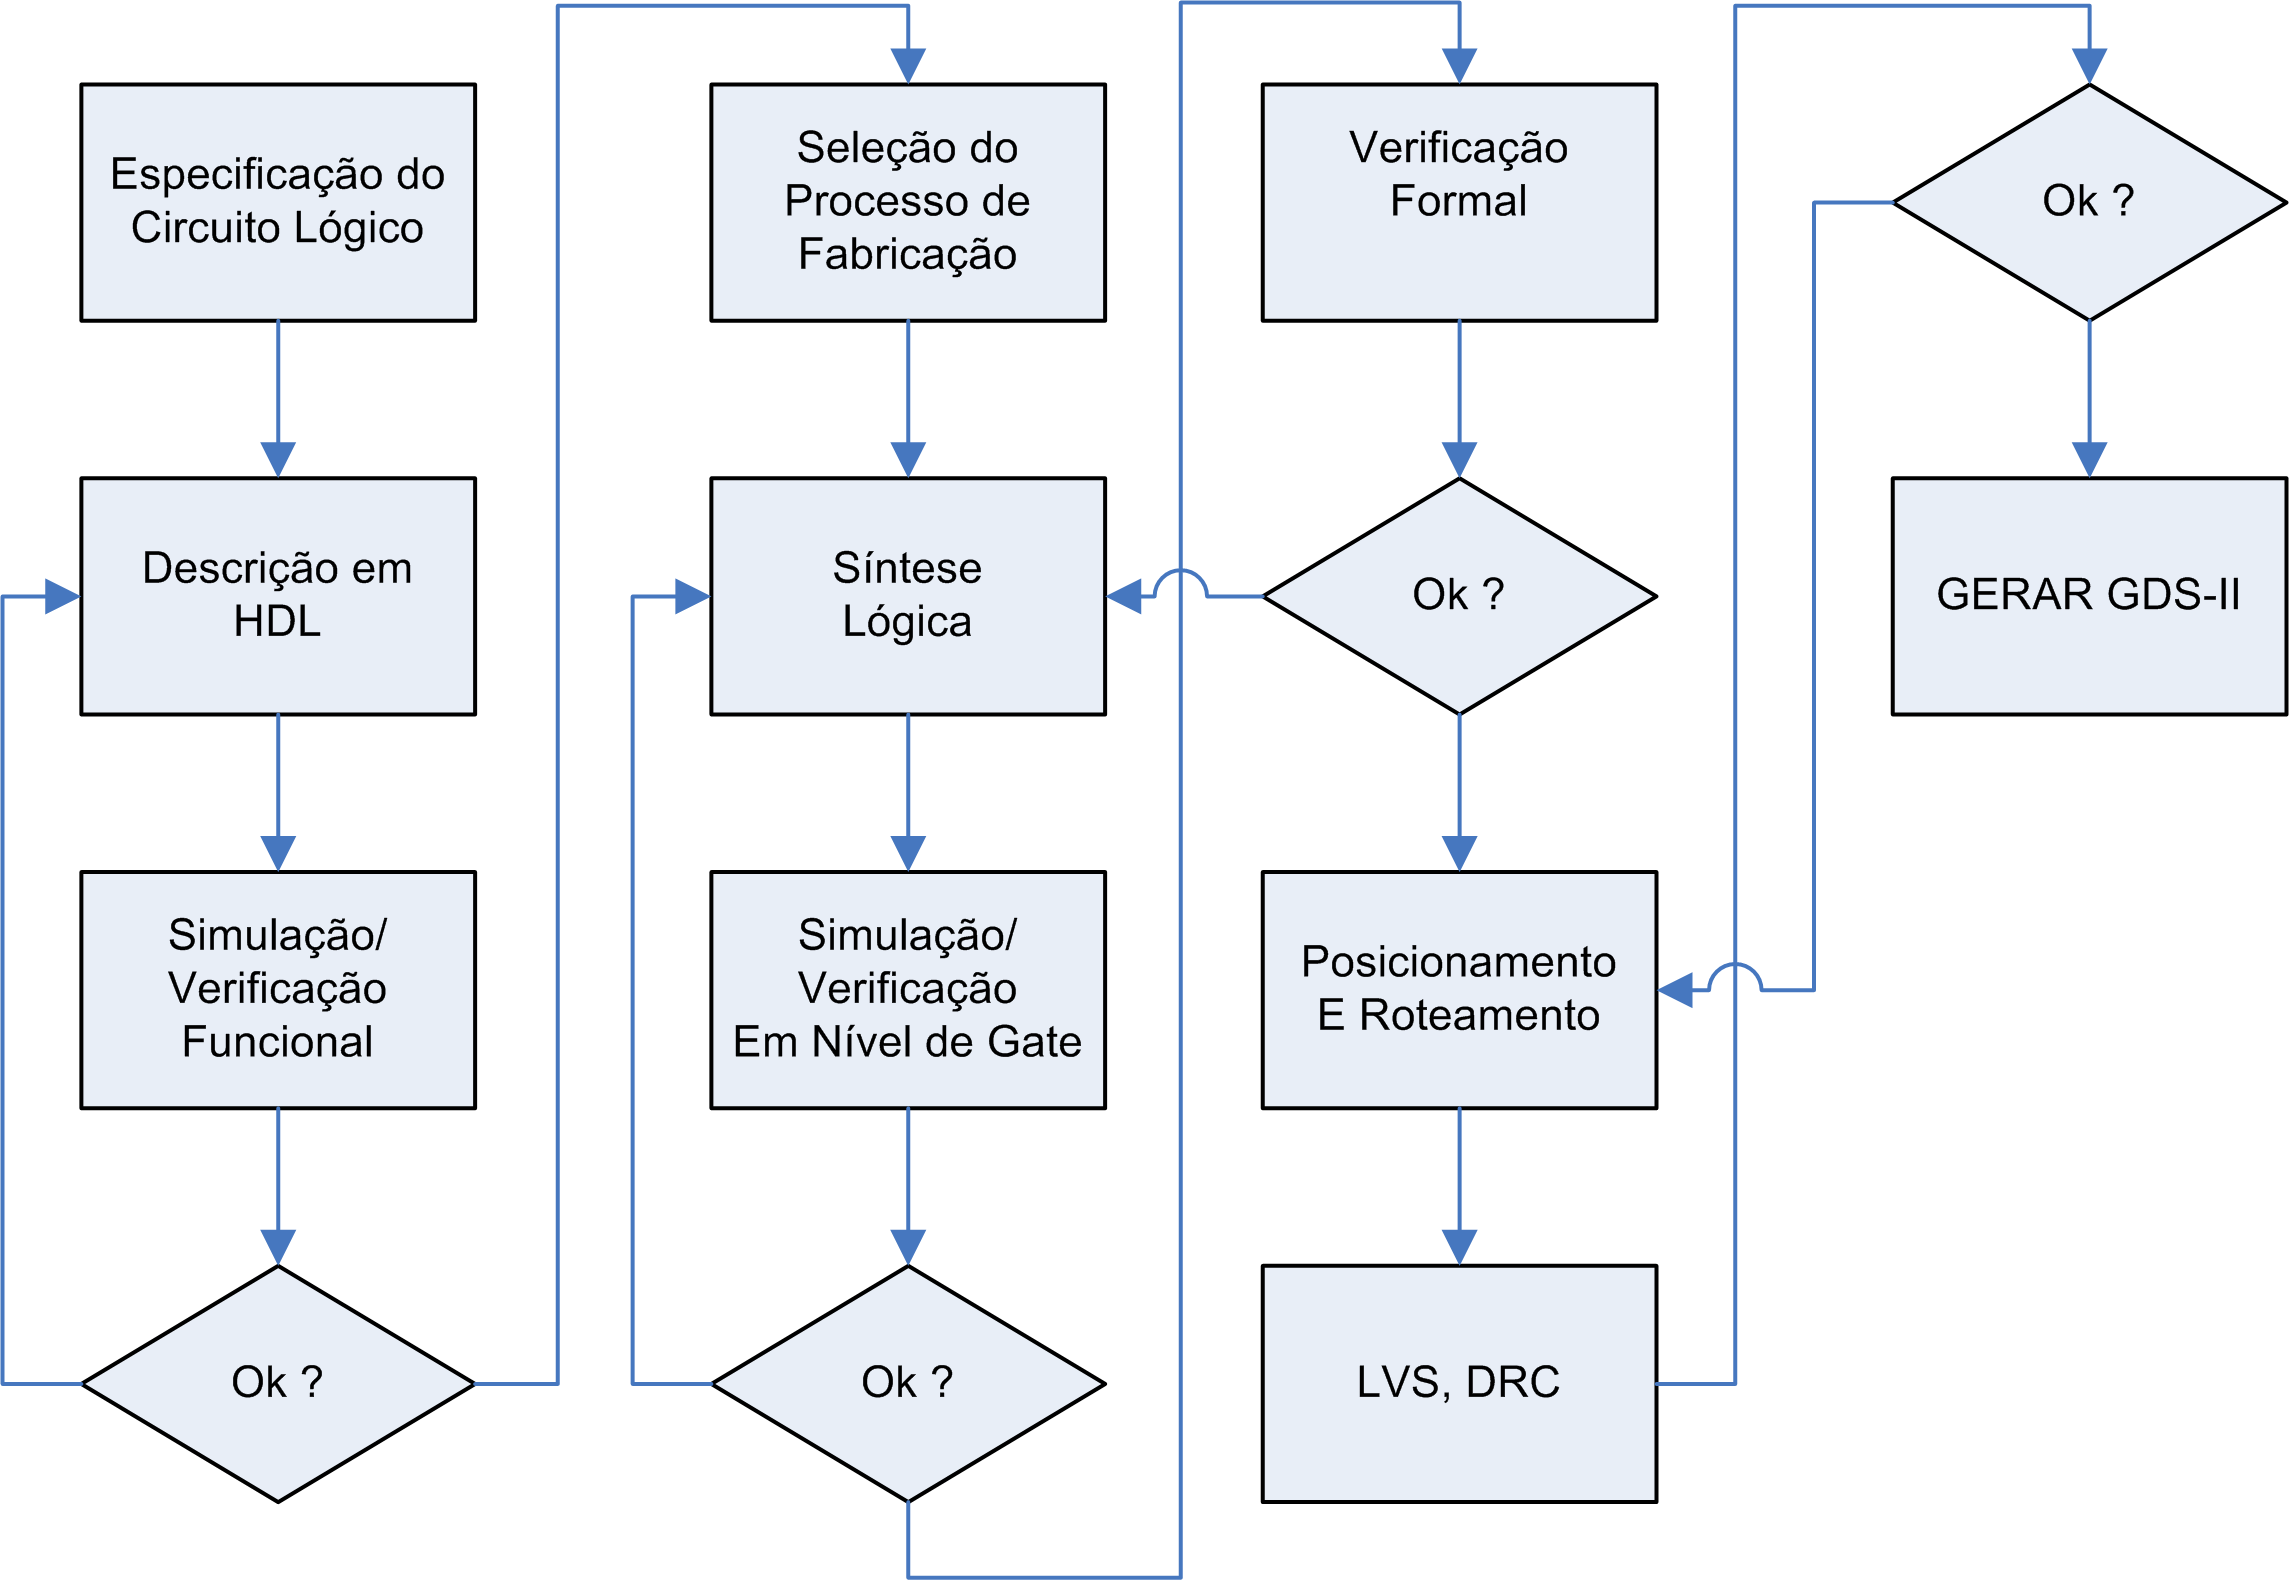
\includegraphics[width=5.0in]{devflow}

\caption{fluxo de desenvolvimento de um circuito l�gico integrado digital, baseado em \emph{standard cells}.}
\label{devflow}

\end{figure}


\subsection{\emph{Standard Cells}}
	A Figura \ref{devflow} mostra o fluxo de desenvolvimento, baseado em \emph{standard cells} de um circuito l�gico integrado digital. Conforme mostrado nesta figura, a sa�da de cada fase, sempre que poss�vel, � confrontada com a especifica��o original ou com a sa�da de fase anterior, de forma a tornar o fluxo de desenvolvimento mais robusto.

	Ap�s gerar a especifica��o de requisitos, conforme descrito anteriormente, o projetista l�gico descrever� o circuito l�gico, para fins de s�ntese, em n�vel RTL (\emph{Register Transfer Level}), na linguagem de sua escolha, VHDL, Verilog ou outra.

	Utilizando-se uma metodologia de verifica��o funcional, a implementa��o desse circuito l�gico deve ser verificada contra a especifica��o original . Uma metodologia de verifica��o que se provou eficaz � a metodologia VeriSC \cite{ipsoc2006}, tendo esta metodologia evolu�do  para a metodologia BVM (\emph{Brazil-IP Verification Me\-tho\-do\-lo\-gy}), que substituiu com vantagens a metodologia VeriSC. Esta metodologia (BVM) foi implementada na linguagem SystemVerilog, utilizando conceitos e biblioteca de OVM (\emph{Open Verification Me\-tho\-do\-lo\-gy}). Esta metodologia tem como objetivo aumentar a produtividade do engenheiro na realiza��o no processo verifica��o funcional \cite{bvm}.

	O circuito l�gico deve ser testado em FPGA, e todo o fluxo de projetos para FPGA dever� ser seguido antes de continuar a sequ�ncia deste fluxo.
	Na fase de s�ntese as restri��es temporais dos sinais, incluindo frequ�ncia de opera��o do circuito, s�o definidas. A sa�da desta fase � um arquivo de descri��o de \emph{hardware} estrutural, baseado nos modelos de portas l�gicas dispon�veis na biblioteca de \emph{standard cells}, que consiste de um \emph{netlist} em formato Verilog.
	Duas a��es podem ser tomadas para garantir que a s�ntese l�gica seja realizada com sucesso: uma simula��o em n�vel de portas l�gicas e uma verifica��o formal.

A verifica��o formal � um processo r�pido e simples do ponto de vista do usu�rio, realizado, por exemplo, com o aux�lio da ferramenta Conformal \cite{formalverification}. A simula��o em n�vel de portas l�gicas � lenta, por consumir muitos recursos computacionais, tendo em vista que cada porta l�gica (podem ser milhares ou milh�es) ser� simulada como uma chave, levando em considera��o caracter�sticas como atraso que est�o dispon�veis no arquivo SDF (\emph{Standard Delay Format}), fornecido junto com as \emph{standard cells}. O projetista poder� optar por n�o realizar esta simula��o, desde que a ferramenta de s�ntese garanta que as restri��es temporais dos sinais sejam cumpridas.
	Para o leiaute do circuito integrado, utiliza-se, por exemplo, a ferramenta Encounter e as seguintes etapas s�o realizadas:
\begin{itemize}
\item primeiramente, a �rea de sil�cio ocupada � definida;
\item os \emph{pads} s�o posicionados nas bordas da regi�o de sil�cio;
\item an�is de alimenta��o (vcc e gnd) s�o desenhados com espa�amento, posicionamento e camada de metal definidos pelo usu�rio;
    \item as portas l�gicas s�o posicionadas, manual ou automaticamente;
    \item a �rvore de \emph{clock} � sintetizada, autom�tica ou manualmente; e
    \item finalmente as conex�es entre as portas l�gicas s�o realizadas, manual ou automaticamente, utilizando �rea e camadas de metal indicadas pelo usu�rio.
\end{itemize}
	A inser��o de portas l�gicas de reserva (\emph{spare gates}) poder� representar um ganho de tempo e de recursos financeiros, caso algum erro seja detectado durante a fase de testes.  Para a manufatura de uma segunda vers�o, ao inv�s se alterar todas as m�scaras, � poss�vel que se precise alterar apenas algumas delas, portanto reduzindo o custo da prototipa��o da segunda vers�o do sil�cio.
	� importante lembrar que na etapa de s�ntese l�gica, as caracter�sticas el�tricas das conex�es s�o consideradas ideais. Ao fazer o leiaute, estas conex�es ideais passam a ser reais. Neste sentido, as caracter�sticas dessas conex�es devem ser ent�o consideradas para verificar se as restri��es temporais e el�tricas est�o sendo cumpridas. Isto � feito com o aux�lio da ferramenta Celt IC.

	Uma vez que as c�lulas fornecidas pela f�brica, para universidades e pequenas empresas, n�o cont�m informa��es a respeito do leiaute interno das c�lulas (pois s�o somente \emph{front-end kits}), torna-se mais complicado fazer o processo de verifica��o final LVS (\emph{Layout Versus Schematics}), que verifica o esquem�tico gerado pela s�ntese l�gica contra o circuito l�gico extra�do a partir do leiaute final (usando o \emph{software} Virtuoso). Um outro processo final de checagem, o DRC (\emph{Design Rule Check}), o qual verifica se as restri��es de leiaute impostas pelo arquivo de tecnologia est�o sendo seguidas, n�o pode ser realizado integralmente devido � falta do leiaute interno das c�lulas. Portanto, o processo como um todo depende das fases anteriores e deve ser correto por constru��o.
	Todos os passos acima podem ser realizados utilizando interfaces gr�ficas e inserindo os dados de entrada manualmente, ou de forma completamente automatizada atrav�s de scripts em TCL (\emph{Tool Control Language}) e Makefile. Este �ltimo � particularmente interessante para refazer o projeto inteiro, ap�s uma modifica��o, com apenas um �nico comando.
	Ent�o o arquivo de manufatura no formato GDSII (\emph{Gerber Data Stream Information Interchange II})  � gerado e pode ser enviado por exemplo, ao Mosis, o servi�o de manufatura da universidade Carolina do Norte para universidades e pequenas empresas. No Mosis, as c�lulas ser�o instanciadas, ou seja, o leiaute interno das \emph{standard cells} ser�o combinados com o leiaute do circuito integrado. Finalmente, o arquivo de leiaute � enviado para o manufaturador do circuito integrado.

\subsection{\emph{Full Custom}}
	No fluxo \emph{full custom}, o circuito l�gico e o leiaute s�o inteiramente desenvolvidos em n�vel de transistor. Com este fluxo de projeto, � necess�ria uma equipe de engenharia, pois cada parte do circuito deve ser manualmente projetada. Como resultado, obt�m-se um projeto muito otimizado em termos de �rea e velocidade de execu��o. A Figura \ref{devflowfullcustom} mostra o fluxo de desenvolvimento de um m�dulo ou de um circuito integrado utilizando um fluxo \emph{full custom}.


\begin{figure}[!htb]
\centering

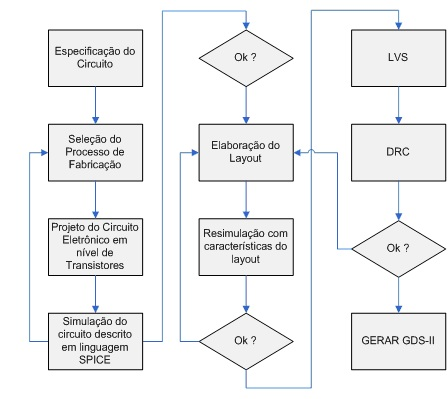
\includegraphics[width=4.5in]{devflowfullcustom}

\caption{fluxo de desenvolvimento de um circuito integrado (l�gico digital ou anal�gico) em n�vel de transistores (\emph{full custom}).}
\label{devflowfullcustom}

\end{figure}




	Ap�s a especifica��o, que deve ser elaborada em forma de um documento de especifica��o de requisitos, seleciona-se o processo no qual o m�dulo ou CI ser� fabricado. Selecionada a tecnologia, a f�brica que det�m a mesma dever� fornecer um kit de desenvolvimento, que cont�m c�lulas b�sicas, como transistores, resistores, capacitores e \emph{pads}. Essas c�lulas s�o usualmente conhecidas como PCELLs ou c�lulas parametriz�veis. S�o parametriz�veis porqu� � poss�vel escolher o comprimento e largura de um transistor antes de instanci�-lo em um circuito.

De posse do kit de desenvolvimento, e a partir da especifica��o, o circuito eletr�nico ser� projetado utilizando as PCELLs dispon�veis no kit de desenvolvimento. Para cada PCELL, o projetista do circuito eletr�nico dever� informar os par�metros da referida c�lula (W, a largura, e L, o comprimento, no caso de transistores). Em fun��o do circuito eletr�nico, incluindo-se os par�metros e modelos das PCELLs, uma simula��o do circuito descrito em linguagem SPICE (\emph{Simulated Program with Integrated Circuits Emphasis}) dever� ser realizada para verificar se o projeto est� de acordo com as especifica��es. O passo seguinte � a elabora��o do leiaute, que comp�e-se do posicionamento das PCELLs e roteamento das conex�es entre estas. Ap�s o leiaute, faz-se uma re-simula��o do circuito, por�m agora incluindo-se as ca\-racte\-r�s\-ti\-cas el�tricas dos componentes parasitas \footnote{Os finos ``fios" met�licos usados para as conex�es, assim como o acoplamento eletromagn�tico das camadas que comp�em o circuito podem gerar dispositivos indesej�veis, tais como indutores e capacitores, os quais s�o classificados como componentes parasitas.} gerados pelas conex�es internas do circuito integrado. Na etapa seguinte, verifica-se se o leiaute est� de acordo com o esquema el�trico projetado atrav�s de um procedimento conhecido como LVS. Finalmente, � verificado se as regras de leiaute impostas pelas restri��es da tecnologia em uso est�o sendo cumpridas; isto � feito por um procedimento identificado como DRC (\emph{Desing Rule Check}).


\section{Reuso de m�dulos}
	M�dulos desenvolvidos utilizando fluxo \emph{full custom} ou \emph{standard cells} em projetos anteriores podem ser reusados em novos projetos, desde que tenham sido desenvolvidos com tal finalidade \cite{ipprocess}. Al�m da redu��o do tempo de desenvolvimento, por serem m�dulos testados em projetos anteriores, diminuem o risco do projeto atual.
	O desenvolvimento para reuso baseia-se no uso de padr�es de interconex�o entre m�dulos de propriedade intelectual. Por exemplo, para m�dulos \emph{soft}, a descri��o l�gica, em n�vel comportamental ou estrutural � reusada. Portanto, o leiaute deve ser refeito para o processo de fabrica��o selecionado. Restri��es temporais e el�tricas dever�o ser garantidas para este novo leiaute do m�dulo.
	M�dulos do tipo \emph{hard} s�o espec�ficos para um processo de fabrica��o e incluem o leiaute do m�dulo. Desta forma, o reaproveitamento � total e n�o � necess�rio refazer e verificar as restri��es temporais e el�tricas para o leiaute do m�dulo.
 %cap 3

\chapter {Processador JOP}
\label{Chapter:JOP}

	\PARstartOne{U}m processador {J}ava � uma implementa��o da m�quina virtual {J}ava. Essa implementa��o n�o � necessariamente completa em \emph{hardware}, pois uma M�quina Virtual {J}ava cont�m fun��es complexas como, por exemplo, escalonamento, gerenciamento e intercomunica��o de processos. O custo de implementar todos esses recursos em \emph{hardware} pode tornar a implementa��o n�o vi�vel. Portanto, o conceito de um processador {J}ava difere de um processador comum, onde apenas elementos de \emph{hardware} est�o envolvidos. Dessa forma, um processador {J}ava � uma implementa��o baseada em \emph{hardware} e, possivelmente, em algum \emph{software}.

	Para um processador {J}ava de tempo real, a caracter�stica de tempo real do processador deve permear tanto o \emph{software}, como o \emph{hardware} deste processador. O JOP (Java Optimized Processor) \cite{jop:jnl:jsa2007} � uma implementa��o em \emph{hardware} e  \emph{software} de uma m�quina virtual {J}ava de tempo real, baseada no perfil J2ME (\emph{Java 2 Micro Edition}) CLDC (\emph{Connected Limited Device Configuration}) e na especifica��o SCJ (\emph{Safety Critical Java}). Este processador pode ser implementado como \emph {soft ip core} em FPGAs Xilinx ou Altera e, diferentemente da JVM (\emph{Java Virtual Machine}) que � uma m�quina CISC (\emph{Complex Instruction Set Computer}), o JOP �, internamente, uma m�quina  RISC (\emph{Reduced Instruction Set Computer}) \cite{jop:tecs:jhal,PattersonHSI},  e portanto, cont�m seu pr�prio conjunto de ins\-tru\-��es.

\section{Implementa��o da JVM no JOP}
	Os \emph{bytecodes} {J}ava s�o decodificados atrav�s de um \emph{pipeline} de ins\-tru\-��es equivalentes nativas do JOP. Para alguns \emph{bytecodes} {J}ava, existe uma equival�ncia biun�voca com ins\-tru\-��es nativas do JOP, as quais s�o executadas em um �nico ciclo de \emph{clock}. \emph{Bytecodes} de m�dia complexidade s�o traduzidos em uma sequ�ncia de ins\-tru\-��es nativas do JOP, encontradas em uma tabela contida em um �rea de mem�ria ROM (\emph{Read Only Memory}), chamada de \emph{JVM microcode} ou Micro-c�digo da M�quina Virtual {J}ava. \emph{Bytecodes} mais complexos, como por exemplo, a instru��o \texttt{new}, s�o implementados na pr�pria linguagem {J}ava e, portanto, traduzidos para sequ�ncias dos demais \emph{bytecodes}, em tempo de exe\-cu\-��o. Para otimizar o desempenho de ins\-tru\-��es espec�ficas, � poss�vel implementar a mesma em \emph{hardware}. O JOP, assim como a JVM original, � uma ``\emph{stack machine}'', ou seja, ao inv�s de realizar opera��es sobre um conjunto de registradores, como ocorre em uma arquitetura x86, as opera��es s�o realizadas sobre os itens que est�o no topo da pilha.


\section{Entrada e sa�da}
	Os dispositivos de E/S do JOP est�o mapeados em mem�ria e, do ponto de vista de \emph{software}, os pinos do JOP s�o acessados pelos m�todos \texttt{Native.rdMem()} e \texttt{Native.wrMem()}. Do ponto de vista do \emph{hardware}, eles s�o implementados pelo \emph{soft ip core} \textbf{scio}, que pode ser visto na Figura \ref{bdjop}.

\begin{figure}[!hb]
\centering

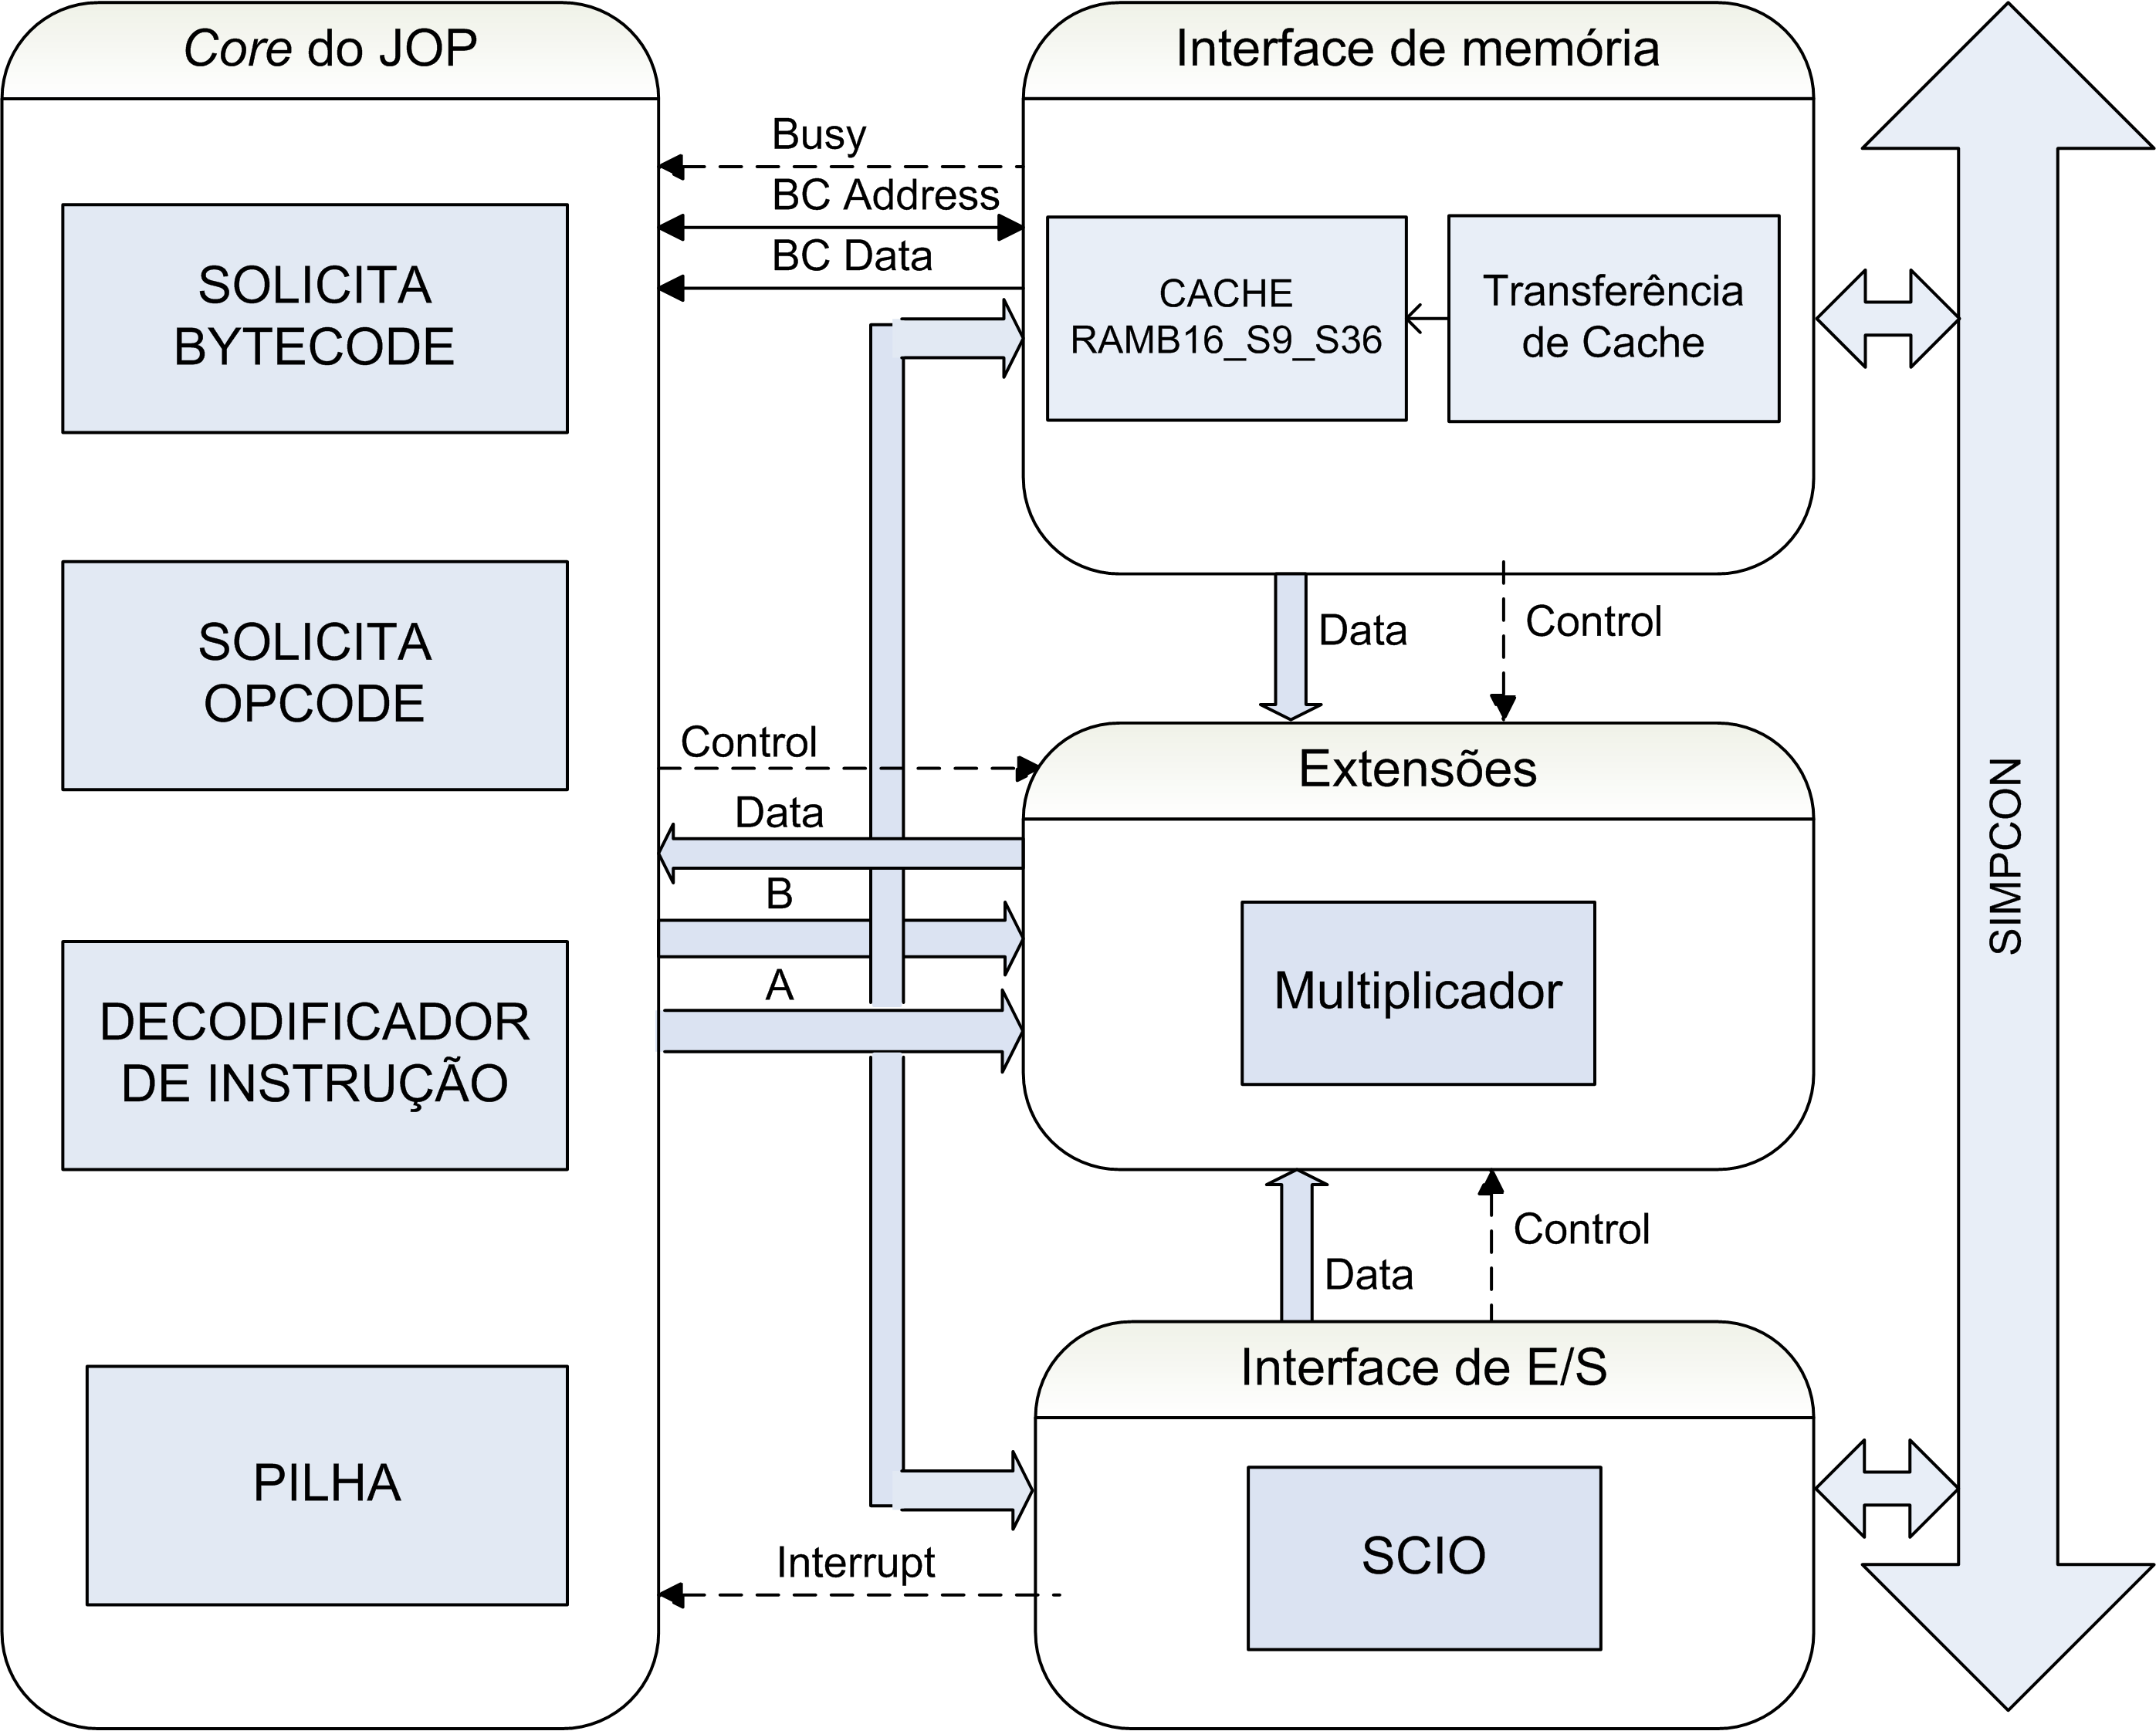
\includegraphics[width=4.5in]{arch_jop_block}

\caption{diagrama de blocos do JOP, adaptado de \cite{JopHandbook}.}
\label{bdjop}

\end{figure}


\section{Interrup��es}
	Interrup��es s�o usadas para sinalizar eventos externos, como por exemplo, detectar que um bot�o foi pressionado. Quando uma interrup��o ocorre, o processador simplesmente p�ra de executar o c�digo atualmente apontado pelo registrador contador de programa, e desvia a exe\-cu\-��o para uma rotina de interrup��o. Al�m disso, o ambiente do processo interrompido � salvo para que esse possa ser restaurado posteriormente. Isso inclui salvar os registros da CPU (\emph{Central Processing Unit}) e os registradores de \emph{status} do processador. Estas a��es tornam poss�vel o retorno da exe\-cu\-��o do c�digo original quando a rotina de interrup��o tiver finalizada.

	No JOP, as interrup��es geram \emph{bytecodes} especiais (\texttt{sys\underline{ }int}), os quais s�o inseridos pelo \emph{hardware} de forma transparente, na sequ�ncia de \emph{bytecodes} a serem executados. Manipuladores de interrup��o podem ser implementados da mesma forma que os \emph{bytecodes}, ou seja, em micro-c�digo ou em {J}ava \cite{jop:interrupt:handler}.


\section{Requisitos de tempo real}
	Aplica��es de tempo real para o JOP s�o explicitamente separadas em duas partes: fase de inicializa��o e fase de miss�o. Na fase de inicializa��o s�o criados todos os objetos que ser�o usados durante toda a exe\-cu\-��o da aplica��o e, portanto, �reas de mem�rias s�o alocadas e inicializadas. Nesta fase n�o existe garantia de tempo real. Na fase de miss�o, as \emph{threads} s�o executadas concorrentemente de acordo com o algoritmo de escalonamento.
\subsection{An�lise de WCET no JOP}
	Por ter sido desenvolvido para ser usado em sistemas embarcados com aplica��es de tempo real, a arquitetura do processador JOP permite calcular com facilidade o WCET (\emph{Worst Case Execution Time}) de uma tarefa.

	A m�quina virtual Java do JOP implementa classes que permitem desenvolver apli\-ca\-��es de tempo real. Essas classes n�o s�o compat�veis com o padr�o RTSJ (\emph {Real Time Specification for Java}) \cite{onjava}, pois apenas um subconjunto deste padr�o � implementado. Embora as �reas de c�digo e de pilha do JOP utilizem mem�ria de \emph{cache}, o modelamento do comportamento da mem�ria \emph {cache} no JOP � perfeitamente previs�vel no tempo. Isso se deve ao fato de, diferentemente de outros processadores, n�o ocorrerem ``\emph{cache misses}'' na \emph{cache} do JOP, ou seja, cada instru��o  solicitada pelo processador � \emph{cache} estar� (exceto as instru��es \texttt{invoke} e \texttt{return}) necessariamente previamente carregada na \emph{cache} \cite{jop:wcet:spe}.
\subsection{Garantia de funcionamento}
	O JOP n�o implementa em sua arquitetura t�cnicas de garantia de funcionamento. Portanto, para aplica��es de tempo real do tipo \emph{hard}, ou seja, que envolvem riscos de vidas humanas, o projetista do sistema dever� assegurar a garantia de funcionamento em n�vel sist�mico. 	No JOP, uma falha de \emph{hardware}, como por exemplo, um \emph{opcode} ilegal ou um erro de paridade de mem�ria, levar� o sistema a um \emph{shutdown} \cite{JopHandbook}.
\section{Arquitetura do JOP}
	O JOP � composto de quatro blocos principais (ver Figura \ref{bdjop}): Interface de mem�ria, \emph{core} do JOP, interface de E/S (\textbf{scio}) e ``extens�es''. O bloco de interface de mem�ria comunica-se com os controladores de mem�rias externas atrav�s do barramento de comunica��o \textbf{simpcon}. Os controladores de mem�ria, por sua vez, comunicam-se, atrav�s dos pinos do processador com as mem�rias SRAM e \emph{flash}. O bloco ``\emph{core} do JOP'' � respons�vel por de\-co\-di\-fi\-car e executar os \emph{bytecodes} fornecidos pela interface de mem�ria e comandar as demais partes do processador. O bloco interface de E/S comunica-se com controladores de E/S, tais como porta USB e Serial RS232, atrav�s do barramento \textbf{simpcon}. Estes controladores de E/S, por sua vez, comunicam-se com os dispositivos do mundo externo atrav�s dos pinos do processador. O bloco de ``extens�es'' serve para agregar fun��es de co-processadores matem�ticos sem realizar modifica��es no n�cleo do processador.

\section{Cache de instru��es de tempo previs�vel}

	Em {J}ava, ou em qualquer linguagem orientada a objetos, um objeto � composto de dados (vari�veis) e das fun��es que operam sobre seus dados, que s�o os m�todos \cite{JavaOO}.

	Solu��es convencionais de \emph{cache}, como por exemplo aquelas baseadas em mapeamento direto ou em mapeamento associativo, introduzem uma imprevisibilidade da exe\-cu\-��o de um algoritmo, o que � incompat�vel com um sistema de tempo real. A solu��o de \emph{cache} de c�digo do JOP, proposta por Schoeberl em \cite{jtrescache}, � completamente diferente das solu��es convencionais e consiste em fazer \emph{cache} de m�todos inteiros, e n�o de ins\-tru\-��es (\emph{bytecodes}) \cite{MartinThesis}.

	No JOP, os bytecodes \texttt{invoke}, \texttt{return} e seus derivados s�o escritos em micro-c�digo (uma sequ�ncia de instru��es do processador RISC interno ao JOP). Essa sequ�ncia de ins\-tru\-��es cont�m uma chamada � instru��o \texttt{stbcrd} e outra chamada � instru��o \texttt{ldbcstart}, as quais disparam a atua��o da \emph{cache} (c�pia da mem�ria RAM externa para mem�ria RAM interna).

	A instru��o \texttt{ldbcstart} insere o endere�o do in�cio do m�todo no topo da pilha. Em seguida, a instru��o \texttt{sbtcrd} � executada e o valor do topo da pilha, o qual neste ins\-tan\-te cont�m o endere�o e tamanho de um m�todo, � transferido para o subsistema de mem�ria. Essa opera��o inicia a transfer�ncia da mem�ria principal para a mem�ria \emph{cache}, atrav�s de um DMA (\emph{Direct Memory Access}). Ne\-nhum outro acesso � mem�ria externa � permitido durante a leitura dos \emph{bytecodes} de um m�todo.

	Com essa abordagem, apenas os bytecodes \texttt{invoke} e \texttt{return} disparam a atua��o da \emph{cache}. Portanto, os �nicos \emph{bytecodes} que possivelmente ter�o um tempo de exe\-cu\-��o vari�vel ser�o \texttt{invoke} e \texttt{return}. Essa varia��o do tempo de exe\-cu\-��o pode ser calculada em fun��o do tamanho do m�todo e das ca\-racte\-r�s\-ti\-cas das mem�rias interna e externa. Essa abordagem facilita a an�lise do WCET das aplica��es do JOP.
\section{Montador de aplica��es}
	O processo de montagem de uma aplica��o para o JOP � descrito no ramo direito da Figura \ref {jopflow}. Conforme pode ser visto no ramo direito desta Figura, ap�s a compila��o, usando o compilador \texttt{javac}, o aplicativo \texttt{jopizer} gera o programa a ser executado pelo JOP.
\begin{figure}[!htb]
\centering
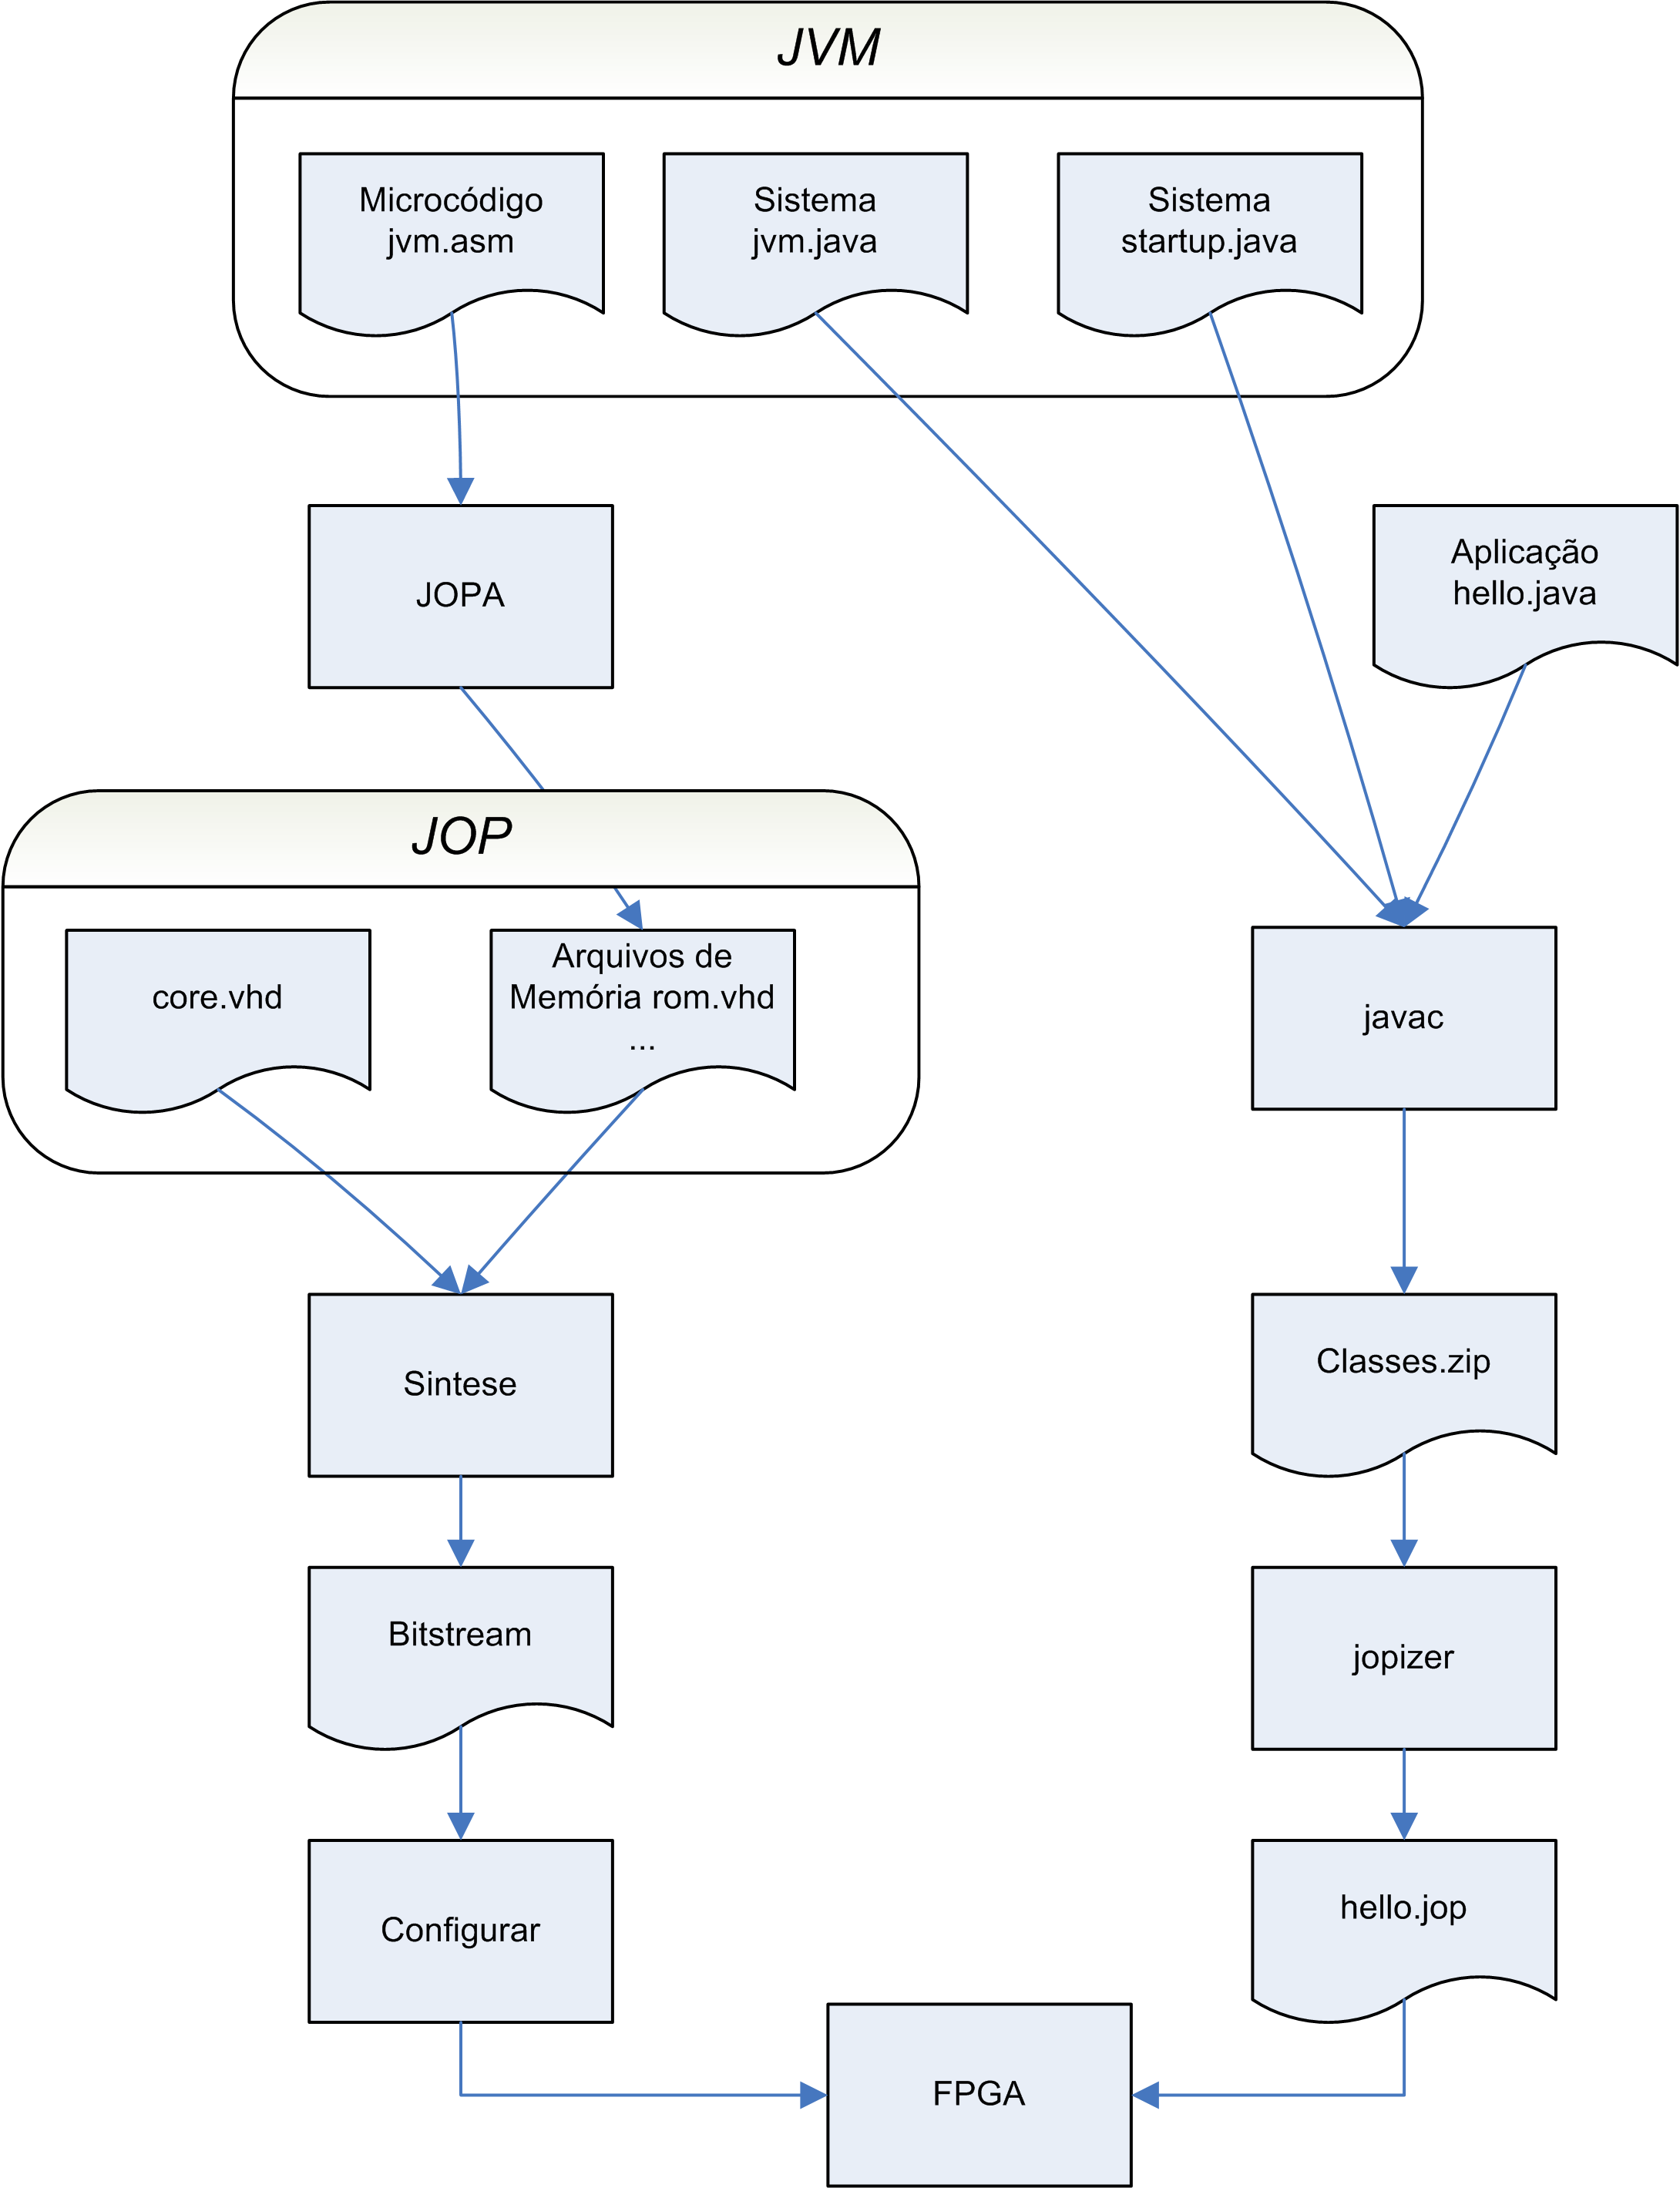
\includegraphics[width=4.5in]{jopflow}
\caption{fluxo de montagem de aplicativo JOP, adaptado de \cite{JopHandbook}.}
\label{jopflow}
\end{figure}
Este programa poder� ser gravado em uma mem�ria \emph{Flash} (aplica��o \emph{standalone}) conectada ao JOP ou enviado a este atrav�s da porta USB (\emph{Universal Serial Bus}) ou Serial RS232. No ramo esquerdo dessa Figura � apresentado o processo de montagem do hardware do JOP, ou seja, a cria��o de um arquivo de configura��o de uma FPGA (\emph{bitstream}) contendo o \emph{soft ip core} JOP.



\section{Documenta��o e portabilidade}	
	Al�m das ca\-racte\-r�s\-ti\-cas t�cnicas do JOP, descritas anteriormente, podemos destacar tamb�m a ampla documenta��o dispon�vel, a sua portabilidade, pois j� foi implementado em diversas placas de desenvolvimento de FPGA (Xilinx e Altera) dispon�veis no mercado. Por �ltimo, mas n�o menos importante, a disponibilidade do c�digo fonte  do JOP para \emph{download} pelo \emph{site} \url {http://www.opencores.org} e licenciado sob a GPL (\emph{Gnu Public License}) vers�o 3.
 Atualmente o JOP � utilizado em dois sistemas comerciais, sendo um deles com requisito de tempo real, e em v�rios sistemas de pesquisa \cite{jop:jnl:jsa2007}. Portanto, o JOP se insere como uma excelente alternativa para plataforma base, de pesquisa e desenvolvimento, de novas t�cnicas de sistemas de tempo real.
 %cap 4

\chapter{JOP Tolerante a Falhas}
\label{Chapter:JOPFT}

\PARstartOne{O}{c�digo} de um programa de um sistema embarcado pode ser armazenado de forma permanente em uma mem�ria n�o vol�til do tipo ROM (\emph{Read Only Memory}), que � um tipo de mem�ria tolerante a SEUs. No entanto, n�o � poss�vel realizar atualiza��es do programa armazenado nesta mem�ria. Por outro lado, as mem�rias do tipo \emph{flash} e SRAM (\emph{Static Random Access Memory}), as quais permitem atualiza��o do programa armazenado, s�o suscept�veis a SEUs \cite{Limabook,flashseu}. Caso os erros de mem�ria de programa armazenados nestas mem�rias n�o sejam tratados, podem ser disseminados para outras partes do sistema e provocar uma falha catastr�fica.

Para detectar e corrigir erros na regi�o de dados de uma mem�ria, existem t�cnicas bastante efetivas implementadas em \emph{software}. Entretanto, as t�cnicas aplicadas em n�vel de \emph{software} para detectar e corrigir erros na regi�o de c�digo de uma mem�ria n�o s�o eficazes, pois, o pr�prio \emph{software} corretor de erros pode estar corrompido (neste tamb�m reside a mem�ria de programa). Nesse sentido, neste Cap�tulo s�o propostas duas t�cnicas,  para detectar e corrigir erros nas mem�rias RAM interna (\emph{cache}) e externa do processador JOP, em n�vel de \emph{hardware} de forma a aumentar a confiabilidade do sistema de \emph{cache} de m�todos descritos no Cap�tulo \ref{Chapter:JOP}.


\section {Ocorr�ncia de evento SEU na mem�ria \emph{cache} interna ao JOP}
     O \emph{floorplan} \footnote{Este \emph{floorplan} do JOP original � um resultado preliminar, de um projeto em desenvolvimento no LESC, que faz parte do programa Brazil-IP.}  do JOP original para a tecnologia XFAB XH035 � apresentado na Figura \ref{jopsilicon}. Os 4 (quatro) blocos inferiores mostrados nesta Figura, identificados por 1, 2, 3 e 4, representam a regi�o ocupada pela mem�ria \emph{cache} do JOP. Em termos percentuais, a �rea do bloco de mem�ria \emph{cache} do JOP equivale a 44,46\% \cite{lesc} da �rea total do JOP original, excetuando-se a �rea ocupada pelos \emph{pads} e an�is de alimenta��o de \texttt{vcc} e \texttt{gnd}. Quando submetido a radia��o, e dado que uma part�cula altamente energizada tenha atingido o processador, existe portanto uma alta probabilidade de que a mem�ria \emph{cache} tenha sido atingida, e possivelmente afetada por um SEU. No evento da ocorr�ncia de um SEU na mem�ria interna (\emph{cache}) do JOP, isto provavelmente levaria o sistema baseado neste processador, a uma falha.
\begin{figure}[!hb]
\centering
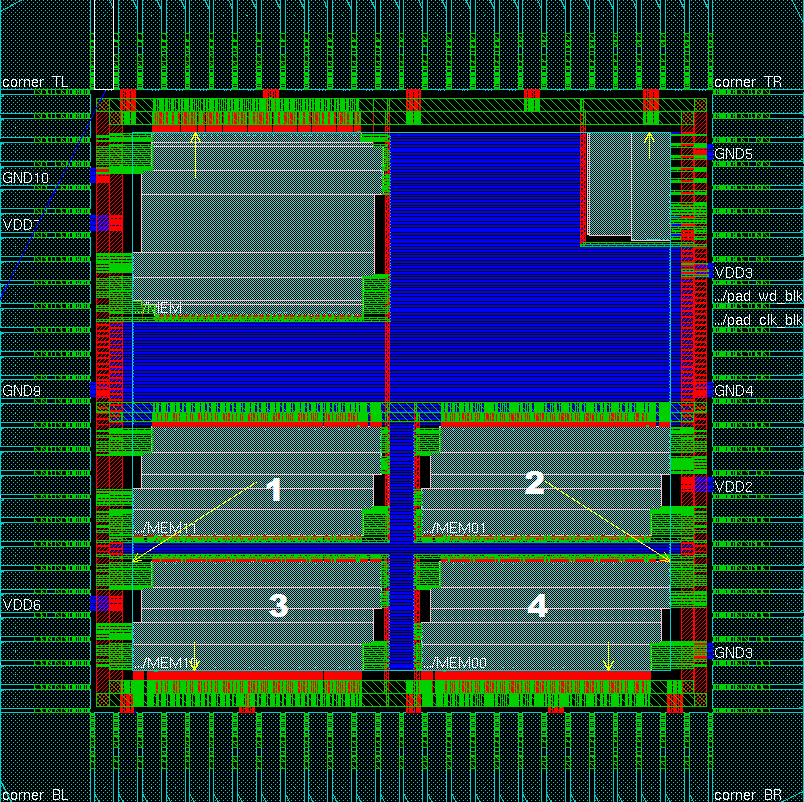
\includegraphics[width=4.0in]{jopsilicon}
\caption{\emph{floorplan} do JOP original, adaptado de \cite{lesc}.}
\label{jopsilicon}
\end{figure}	

\section {T�cnica de Prote��o de Instru��es (TPI)}

    Para lidar com o problema abordado anteriormente, prop�e-se o uso de blocos detectores e corretores de erros na mem�ria \emph{cache} do JOP \cite{tpi}.


	A t�cnica de prote��o de instru��es (ou TPI) detecta e corrige erros ocorridos nos \emph{bytecodes}, desde o armazenamento destes na \emph{cache} at� o in�cio de sua execu��o pelo \emph{core} do JOP. O erro � detectado e corrigido imediatamente antes do \emph{core} iniciar a exe\-cu\-��o do \emph{bytecode}. Portanto, essa � uma t�cnica de verifica��o de �ltimo instante (\emph{last minute check}) e que mascara a falha \cite{helanothesis}.

   Utiliza-se redund�ncia da \emph{cache} interna para proteger as instru��es armazenadas nesta mem�ria. As instru��es s�o armazenadas durante um curto per�odo de tempo na mem�ria \emph{cache}, existindo uma baixa probabilidade de que dois \emph{bits} de uma mesma instru��o sejam invertidos antes que outra instru��o seja escrita nesta mesma posi��o de mem�ria. Esta id�ia � similar ao princ�pio no qual se baseia a t�cnica de \emph{scrubbing} para prote��o da mem�ria de configura��o de FPGAs, ou seja, antes que ocorram dois SEUs, aquela posi��o de mem�ria deve ter sido reescrita com o mesmo, ou com outro dado \cite{Limabook,CRCFpga}. Baseado neste princ�pio, escolheu-se um codificador de Hamming SECSED (\emph{Single Error Correction Single Error Detection}) para co\-di\-fi\-ca\-��o dos dados da mem�ria \emph{cache}.

\subsection{Fluxo dos \emph{Bytecodes} no JOP x Fluxo dos \emph{Bytecodes} no FT-JOP}

   A mem�ria \emph{cache} do processador JOP � uma mem�ria com duas portas para leitura e/ou escrita, identificadas como porta A e porta B. A porta A desta mem�ria permite acessar 2048 endere�os, cada um contendo uma palavra de 8 \emph{bits} de dados. A porta B permite acessar 512 endere�os, cada um contendo 32 \emph{bits} de dados. No projeto original do JOP, os dados s�o transferidos da mem�ria externa (SRAM ou \emph{flash}) para a mem�ria \emph{cache} atrav�s da porta B e, a partir da porta A, os \emph{bytecodes} s�o transferidos para o \emph{core} do JOP que ir� executar a instru��o. Portanto, no JOP original, as instru��es seguem o seguinte fluxo: mem�ria externa, \emph{cache} e n�cleo do JOP.

   O projeto do JOP foi modificado neste trabalho, de modo que simultaneamente � escrita de um \emph{bytecode} (tamanho de 8 \emph{bits}) na mem�ria \emph{cache}, 4 \emph{bits} extras de redund�ncia (\emph{bits} de Hamming) s�o calculados e armazenados em uma mem�ria \emph{cache}, de redund�ncia, que se posiciona em paralelo com a \emph{cache} original, conforme mostrado na Figura \ref{jopmodificado} - parte B. Esses \emph{bits} extras s�o calculados por um \emph{core} escrito em RTL (\emph{Register Transfer Level}), que implementa um codificador de Hamming.

\begin{figure}[!htb]
\centering
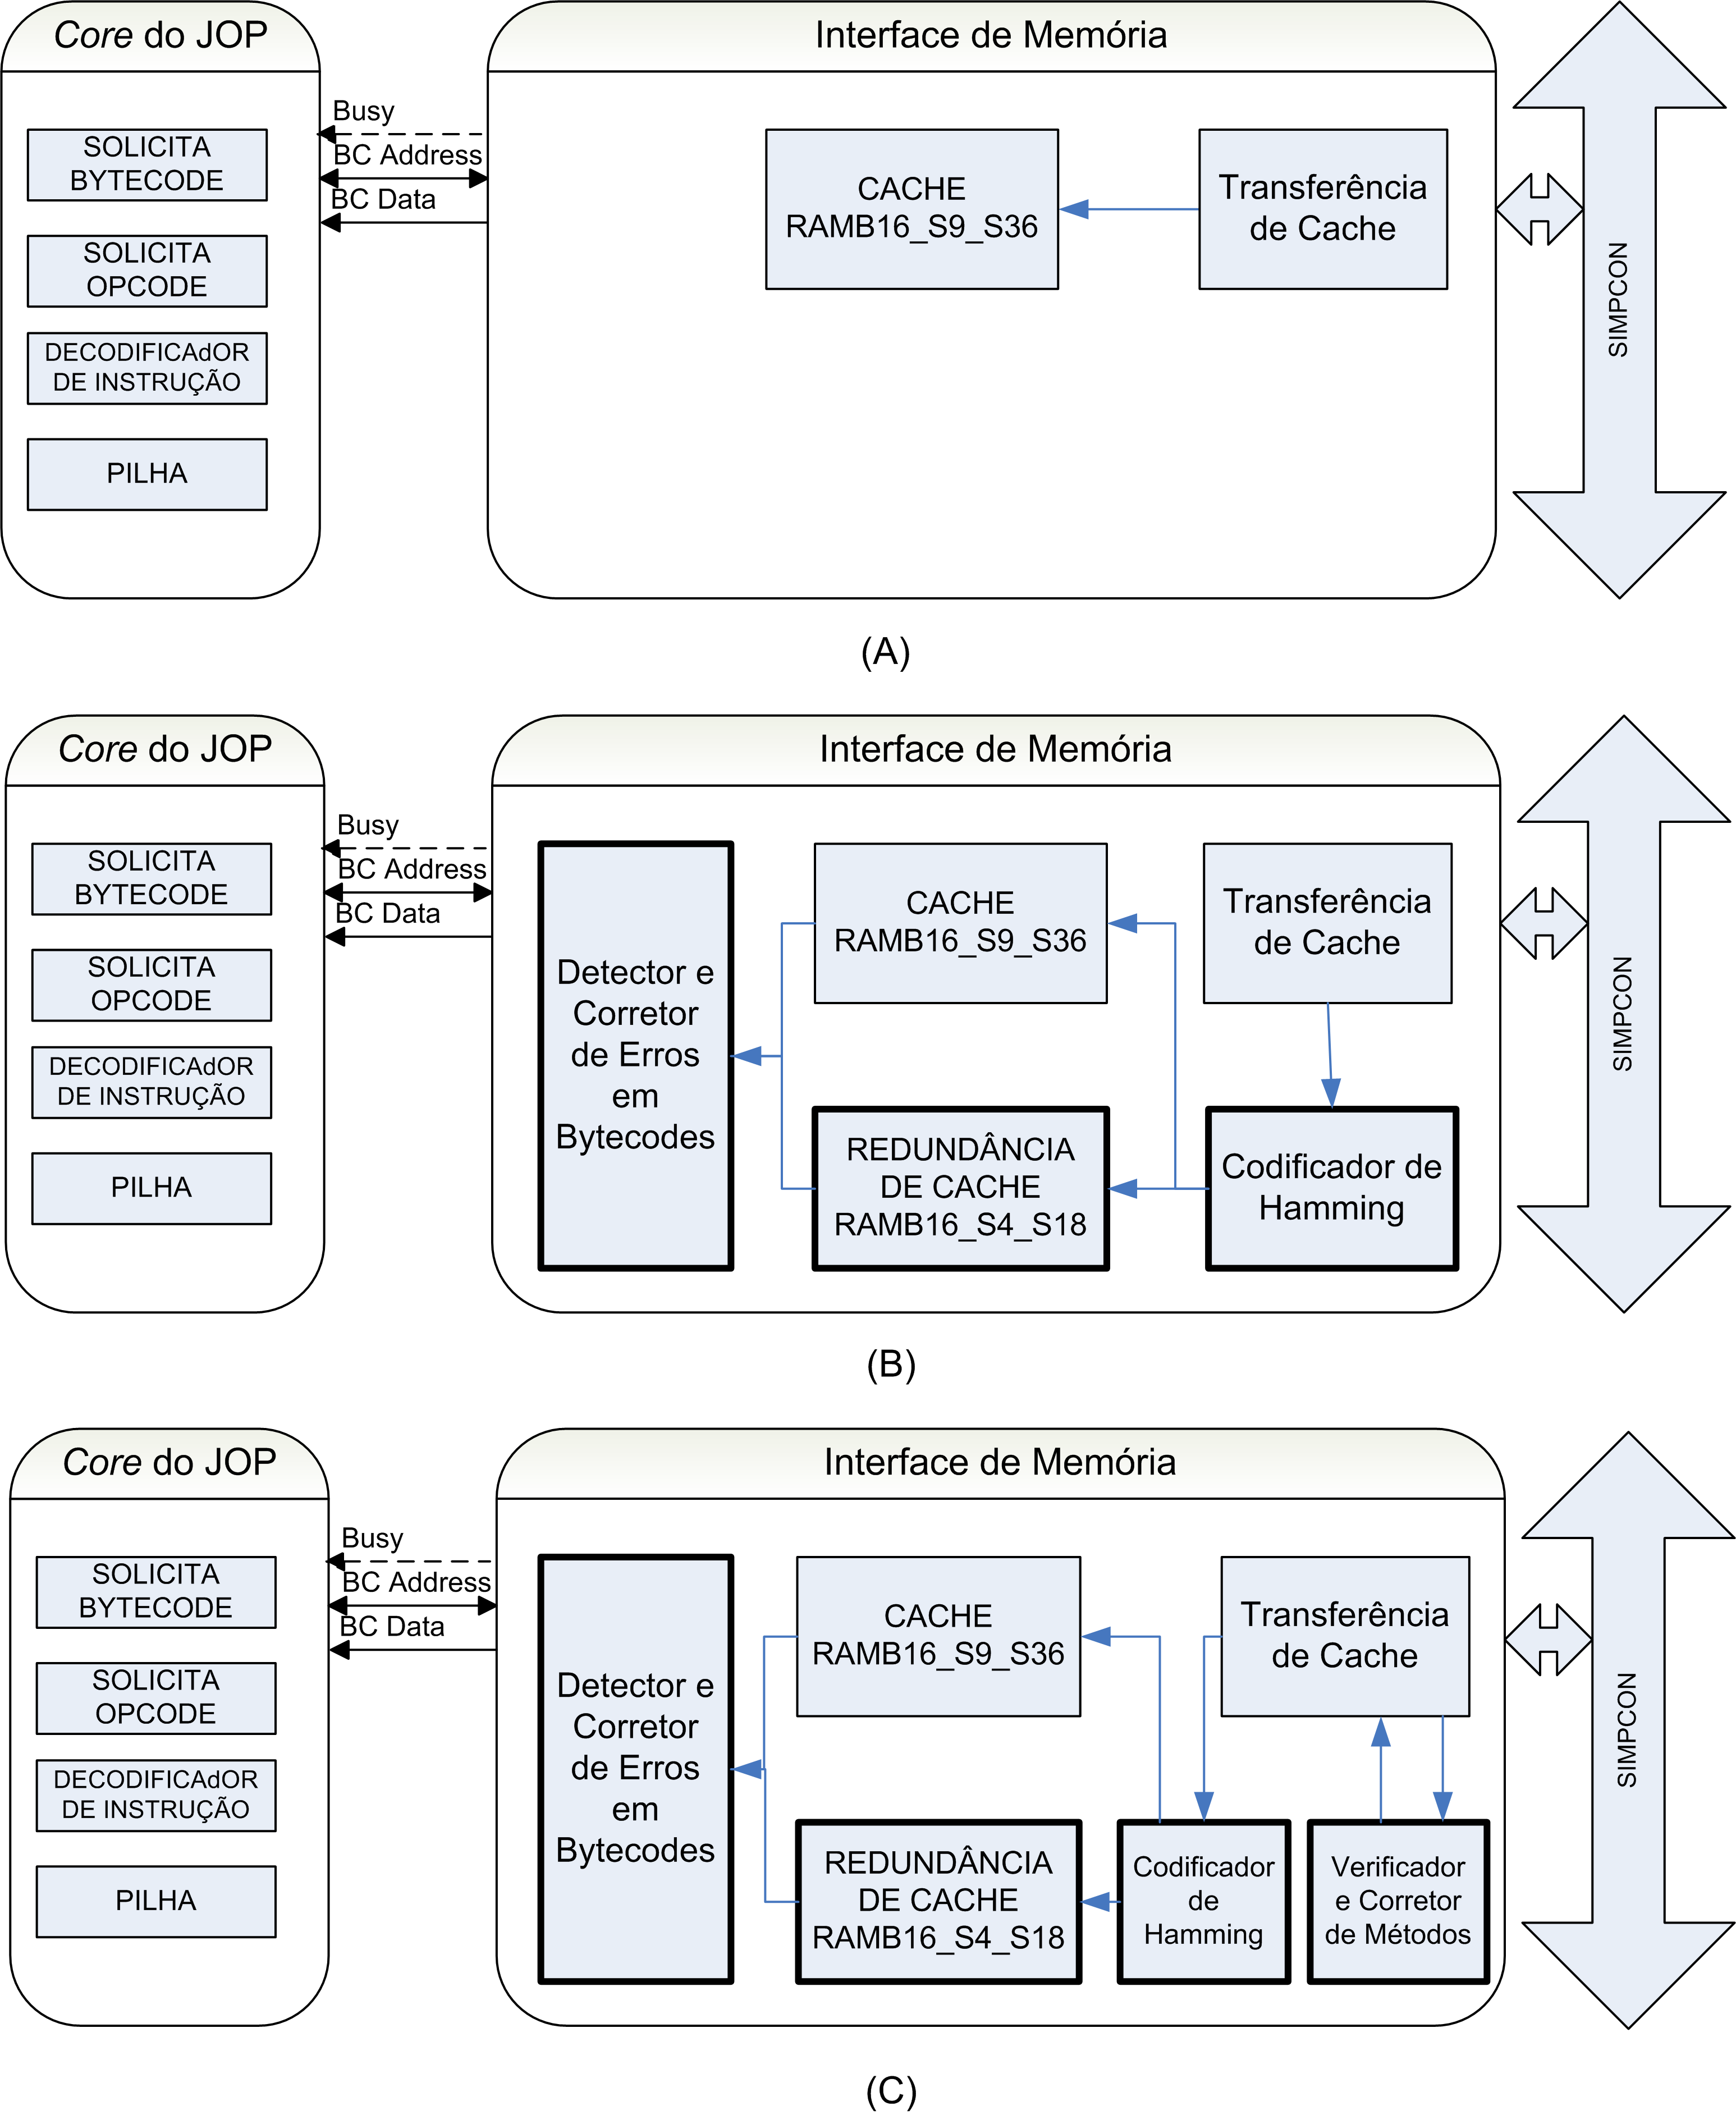
\includegraphics[width=4.1in]{jopmodificado}
\caption{Configura��es do JOP - (A) JOP original  (B) JOP Original e TPI  (C) JOP Original, TPI e TPM.}
\label{jopmodificado}
\end{figure}	

	Foram desenvolvidos 2 (dois) \emph{ip cores} e especificada uma mem�ria interna da FPGA para a implementa��o da T�cnica de Prote��o de Instru��es (TPI), os quais podem ser vistos na Figura \ref{jopmodificado} (parte B). A seguir, listamos e descrevemos cada um destes blocos:
\begin{enumerate}
\item codificador de Hamming;
\item detector e corretor de erros em \emph{bytecodes} (Decodificador de Hamming); e
\item redund�ncia de \emph{cache} (RAMB16\underline{ }S4\underline{ }S18).
\end{enumerate}

   \subsection{Codificador de Hamming}

   Foi desenvolvido um bloco codificador de Hamming SECSED, que � inserido entre a mem�ria externa e a mem�ria \emph{cache} do JOP. Este bloco recebe 32 \emph{bits} de dados (ou quatro instru��es, pois cada uma tem 8 \emph{bits}) e gera uma sa�da de 48 \emph{bits}.

  \subsection{Bloco extra de mem�ria}
    Al�m do bloco codificador de Hamming, foi acrescentado ao JOP uma mem�ria, tamb�m de porta dupla, para armazenar os \emph{bits} extras gerados pelo codificador de Hamming. Esta � uma mem�ria do tipo RAMB16\underline{ }S4\underline{ }S18. De acordo com a Tabela \ref{tabelaramb}, a porta $A$ desta mem�ria permite acessar 4096 endere�os, cada um contendo uma palavra de 4 \emph{bits} de dados, e a porta B permite acessar 1024 endere�os, cada um contendo 16 \emph{bits} de dados.

\begin{table}[!htb]
\begin{center}
%% increase table row spacing, adjust to taste
\renewcommand{\arraystretch}{1.3}
% if using array.sty, it might be a good idea to tweak the value of
% \extrarowheight as needed to properly center the text within the cells
\caption{componentes de mem�ria utilizados.}
\label{tabelaramb}
% Some packages, such as MDW tools, offer better commands for making tables
% than the plain LaTeX2e tabular which is used here.
\begin{tabular}{|c|c|c|}	\hline
% &  &  & Port A &  &   & &  Port B &  &  & \\ \hline
Componente & Porta A &  Porta B   \\ \hline
RAMB16\underline{ }S9\underline{ }S36 & 2048 x 8 &   	512 x 32     \\ \hline
RAMB16\underline{ }S4\underline{ }S18 & 4096 x 4 &  	1024 x 16   \\ \hline
\end{tabular}
\end{center}
\end {table}
   \subsubsection{Decodificador de Hamming}
	Imediatamente ap�s a mem�ria \emph{cache} fornecer um \emph{bytecode} para o \emph{core} do JOP, por�m antes de ser executado, um \emph{core} decodificador de Hamming l� os 4 \emph{bits} armazenados na \emph{cache} de redund�ncia, conforme mostrado na Figura \ref{jopmodificado} - parte B. Com base nesses 12 (doze) \emph{bits}, oito \emph{bits} do \emph{bytecode} mais quatro \emph{bits} de Hamming, esse \emph{core} verifica se houve alguma invers�o de bit em algum dos \emph{bits} do \emph{bytecode}. Em caso afirmativo, isto significa que houve uma falha. Neste caso, o \emph{core} decodificador de Hamming corrige automaticamente o \emph{bytecode}, desde que apenas um bit tenha sido invertido. Finalmente, o \emph{bytecode} correto � entregue para a execu��o por parte do \emph{core} do JOP.


%% DESCREVER O CORE DE HAMMING
%% Foi desenvolvido tamb�m um core decodificador de Hamming.


%% EXPLICAR SOBRE BAIXA PROBABILIDADE DE INVERS�O DE MAIS DE UM BIT
%% C�DIGO RS MUITO PESADO
	
\section {Ocorr�ncia de evento SEU na mem�ria externa ao JOP}
	Durante a inicializa��o do processador JOP, todo o c�digo � transferido da mem�ria \emph{flash} para a mem�ria RAM. Ap�s o c�digo estar na mem�ria RAM, o sistema de \emph{cache} transfere, sob demanda, m�todos inteiros da mem�ria externa para a mem�ria de \emph{cache} interna. Por �ltimo, ap�s um m�todo estar completamente carregado na mem�ria interna, o \emph{core} solicita e executa os \emph{bytecodes}, um a um.
    No caso de ocorr�ncia de um SEU na mem�ria externa (\emph{Flash} ou RAM) do JOP, isto provavelmente levaria o sistema baseado neste processador, a um defeito.


\section{T�cnica de prote��o de m�todos}


%% DESCREVER O PROBLEMA ... PORQUE PROTEGE M�TODOS ETC.
	Para proteger o JOP deste tipo de ocorr�ncia, foi desenvolvida neste trabalho a t�cnica de prote��o de m�todos. Esta t�cnica detecta e corrige erros ocorridos desde o processo de transfer�ncia do c�digo da mem�ria \emph{flash} at� a grava��o deste na mem�ria \emph{cache}. O erro � detectado e corrigido antes de iniciar a exe\-cu\-��o do m�todo. Portanto, essa � uma t�cnica de checagem antecipada (\emph{early check}).


\subsection{Software para adicionar CRC aos m�todos}
\label{section:addcrc}
    Foi desenvolvido um software (de nome \texttt{ProtegeMetodo}) para calcular o CRC32 de cada m�todo, e adicionar este dado ao final de cada m�todo, no arquivo a ser gravado na mem�ria de programa do JOP.
	Portanto, essa t�cnica requer que o CRC  (\emph{Cyclical Redundancy Check}) \cite{crc1} de todos os m�todos  contidos no programa da aplica��o sejam calculados e anexados � mem�ria de c�digo do JOP. Isto � feito pelo aplicativo \texttt{ProtegeMetodo} na fase de montagem do programa.


Para ilustrar o funcionamento da t�cnica de prote��o de m�todos, considera-se o programa \texttt{HelloWorld.java} mostrado abaixo, o qual envia uma mensagem para a porta serial do processador JOP.
\verbatiminput{HelloWorld.java}

Como pode ser visto neste c�digo fonte do programa \texttt{HelloWorld}, o m�todo \texttt{main} invoca o m�todo \texttt{println} da classe \texttt{System.out}. Apresenta-se a seguir o c�digo fonte de baixo n�vel do m�todo \texttt{main} gerado pelo compilador \texttt{javac}.
\verbatiminput{HelloWorld.bc}
Nota-se que os \emph{bytecodes} \texttt{getstatic\underline{ }ref}, \texttt{ldc}, \texttt{invokevirtual} e \texttt{return} s�o utilizados para a implementa��o do m�todo \texttt{main}. Os \emph{opcodes} relativos a estas instru��es, assim como a quantidade de operandos que cada uma dessas instru��es deve receber s�o mostrados na Tabela \ref{tabelaopcodes}.
\begin{table}[!htb]
\begin{center}
%% increase table row spacing, adjust to taste
\renewcommand{\arraystretch}{1.3}
% if using array.sty, it might be a good idea to tweak the value of
% \extrarowheight as needed to properly center the text within the cells
\caption{instru��es utilizadas no m�todo \texttt{main} do programa HelloWorld.java.}
\label{tabelaopcodes}
% Some packages, such as MDW tools, offer better commands for making tables
% than the plain LaTeX2e tabular which is used here.
\begin{tabular}{|c|c|c|}	\hline
Instru��o da JVM    &   Opcode   & Operandos   \\	\hline
\texttt{getstatic\underline{ }ref}   & 224 & 2   \\ 	\hline
\texttt{ldc}   & 18 & 1 \\ 	\hline
\texttt{invokevirtual}   & 182 & 2 \\ 	\hline
\texttt{return}   & 177 & 0 \\ 	\hline
\end{tabular}
\end{center}
\end {table}
Mostra-se abaixo o c�digo de m�quina gerado pelo compilador, o qual deve ser gravado na mem�ria externa do processador JOP.
\verbatiminput{HelloWorld.jop}
Neste c�digo de m�quina, cada linha cont�m uma palvra de 32 \emph{bits} e portanto, 4 \emph{bytes}. Cada um destes \emph{bytes} pode representar um \emph{opcode} ou um operando de um \emph{opcode}. Por exemplo, na linha 1, observa-se o opcode 224, que de acordo com a Tabela \ref{tabelaopcodes}, representa a instru��o \texttt{getstatic\underline{ }ref}. Ainda na linha 1, encontram-se os \emph{bytes} 0 e 148, que s�o operandos da instru��o anterior (\texttt{getstatic\underline{ }ref}), e o \emph{byte} 18 que representa a instru��o \texttt{ldc}. Mostra-se a seguir o c�digo de m�quina gerado pelo programa \texttt{ProtegeMetodo} para este exemplo.
\verbatiminput{HelloWorldCRC.jop}
Como pode ser visto neste c�digo gerado pelo programa \texttt{ProtegeMetodo}, uma palavra de 32 \emph{bits} extra foi adicionada ao c�digo de m�quina. Esta palavra extra � o resultado do algoritmo CRC32 aplicado sobre todas as palavras que comp�em o m�todo.


\subsection{Verificador da integridade dos m�todos}


	Sempre que um novo m�todo for carregado na mem�ria \emph{cache} de c�digo, a \emph{cache} de m�todos tolerante a falhas e de tempo previs�vel faz, em paralelo com a carga do m�todo, o c�lculo do CRC deste. Para realizar este c�lculo foi adicionado ao bloco de interface de mem�ria do JOP, um bloco verificador e corretor de m�todos, conforme apresentado na Figura \ref{jopmodificado} - parte C. Ao final da carga do m�todo na mem�ria \emph{cache}, por�m antes de execut�-lo, o valor calculado do CRC do m�todo � comparado com o valor do CRC do m�todo lido da mem�ria. Nessa situa��o, caso os valores do CRCs do m�todo, lido da mem�ria e calculado sejam diferentes, isto significa que ocorreu uma falha no sistema.


	Logo ap�s a detec��o da falha, uma exce��o � gerada e o m�todo em falha � impedido de ser executado, evitando assim que um erro seja gerado por essa falha. � importante salientar que esta t�cnica detecta uma falha antes que a mesma possa causar um erro e, portanto, n�o causa um defeito no sistema.

	Quando uma falha � detectada, o conte�do do m�todo do pr�prio CRC pode estar corrompido, pois, os dois valores (lido e calculado) est�o armazenados na mesma mem�ria. No entanto, estatisticamente � muito mais prov�vel que o m�todo esteja corrompido e n�o o CRC. Uma poss�vel estrat�gia para aumentar a confiabilidade e detectar qual dos dois est� realmente corrompido, seria armazenar o CRC de forma redundante, ou seja, em duas ou mais �reas distintas da mem�ria SRAM.

	Com a modifica��o proposta por esta t�cnica, o \emph{cache} de m�todos do JOP continua a ter previsibilidade de tempo, pois, n�o houve altera��es no n�cleo do processador ou em seu \emph{pipeline}, mas somente na interface de mem�ria. Ap�s a detec��o do erro, duas abordagens podem ser seguidas pelo projetista do sistema. Na primeira, o projetista pode optar por n�o tentar corrigir o m�todo e levar imediatamente o sistema a um modo de falha segura. Numa segunda abordagem, indicada para sistemas de tempo real do tipo \emph{hard}, a an�lise de WCET deve considerar, al�m do tempo de c�lculo do CRC, o tempo de corre��o do m�todo, que pode ser feita, por exemplo, a partir de uma mem�ria de programa secund�ria (externa ao JOP). Na primeira abordagem, o sistema tem um WCET menor que na segunda; em compensa��o possui uma confiabilidade menor do que o segundo caso, por�m ainda maior que a \emph {cache} de m�todos original do JOP.



\subsection{Percep��o da falha em n�vel sist�mico}
	Uma falha de \emph{hardware} no JOP original, como por exemplo, um \emph{opcode} ilegal, leva o sistema a um \emph{shutdown} \cite{JopHandbook}. Neste trabalho, o processador foi modificado para que, na ocorr�ncia de uma falha de \emph{hardware}, uma exce��o seja gerada. Segue abaixo um exemplo de c�digo de como o programador deve fazer o tratamento de uma falha de \emph{hardware}.
\verbatiminput{exception}

\section{Aplicabilidade das t�cnicas de TPI e TPM}

As duas t�cnicas propostas neste Cap�utlo (TPI e TPM) podem ser utilizadas para aumentar a confiabilidade do processador JOP, tanto em FPGA, como em tecnologia CMOS.
No entanto, para o caso de FPGAs, � necess�rio aplicar em conjunto com as t�cnicas de TPI e/ou TPM, uma t�cnica que proteja a mem�ria de configura��o da FPGA contra SEUs, como por exemplo a t�cnica de \emph{scrubbing} \cite{Limabook}, ou ainda a t�cnica de vota��o de CRC de frames da FPGA,  proposta no trabalho desenvolvido por \cite{CRCFpga}. � importante ressaltar que estas duas �ltimas t�cnicas (\emph{scrubbing} e vota��o de CRCs) n�o protegem as mem�rias BRAMs (Bloco de mem�ria RAM) da FPGA utilizadas pelo processador. Portanto, para o caso de FPGAs, as t�cnicas de prote��o da \emph{cache} e de prote��o de configura��o da FPGA s�o complementares.
Para o caso de tecnologia CMOS, as t�cnicas de TPI e TPM podem ser aplicadas diretamente.


\section{S�ntese do JOP em Sil�cio}

At� a escrita desse trabalho, apenas foi detectada a implementa��o do JOP para FPGAs. Neste sentido, uma outra contribui��o deste trabalho � elencar as modifica��es necess�rias e/ou desej�veis, nos c�digos fontes do JOP, para a prototipa��o do JOP em tecnologia CMOS. Esta contribui��o adicional representa um grande passo na evolu��o desse processador.

\subsection {Sistema de verifica��o funcional}

    Conforme visto no Cap�tulo \ref{Chapter:PCILD}, uma das etapas important�ssimas do fluxo de projeto de circuitos integrados � a verifica��o funcional do chip. Os c�digos fontes do JOP incluem somente um \emph{testbench} de simula��o para execu��o do programa HelloWorld discutido na Se��o \ref{section:addcrc}. Neste sentido, para a prototipa��o do JOP em tecnologia CMOS, o primeiro passo � definir e implementar um sistema eficiente de verifica��o funcional. No Cap�tulo \ref{Chapter:PCILD} � feita uma descri��o sucinta da metodologia BVM \emph{Brazil-IP Verification Methodology}, a qual poderia ser aplicada para o JOP.

\subsection {Substitui��o das BRAMs}

De acordo com o que foi visto nos Cap�tulos \ref{Chapter:PCILD} e \ref{Chapter:JOP}, a implementa��o do JOP em FPGA utiliza dois blocos de mem�ria RAM dispon�veis na FPGA, um para implementa��o do bloco \emph{stack} e outro para implementa��o da mem�ria \emph{cache}. Al�m das duas mem�rias RAM, o JOP necessita de uma mem�ria ROM para armazenamento da implementa��o e mapeamento de alguns \emph{bytecodes} Java em micro-c�digo. Atrav�s do Servi�o Mosis \cite{mosis} ou mesmo em contato direto com o manufaturador do chip, � poss�vel conseguir os softwares geradores de mem�ria para a tecnologia escolhida. Estes devem ser utilizados para gerar as mem�rias do JOP.

Os softwares geradores de mem�ria, al�m de gerarem os blocos de mem�ria, geram um modelo (escrito em uma HDL) do bloco de mem�ria gerado. Estas mem�rias s�o, possivelmente, diferentes em termos de l�gica de acesso e temporiza��o, daquelas encontradas nas FPGAs. Assim, faz-se necess�rio modificar o JOP para que este trabalhe corretamente com as mem�rias da tecnologia na qual ser� fabricado. Para realiza��o desta tarefa, o modelo da mem�ria gerado pelo \emph{software} ser� bastante �til.


\subsection {Inicializa��o da \emph{Stack} RAM}

    Para compreender a inicializa��o da \emph{stack} RAM, deve-se lembrar que para um sistema implementado em FPGAs baseadas em SRAM, � necess�rio gravar o \emph{bitstream} na FPGA sempre que o sistema inicializa. No caso do JOP, sua implementa��o se utiliza desta fase (inicializa��o) para, al�m de gravar a configura��o da FPGA, inicializar a mem�ria \emph{stack} RAM do JOP. Neste sentido, para a implementa��o do JOP em tecnologia CMOS, faz-se necess�rio projetar um circuito l�gico capaz de inicializar a mem�ria \emph{stack} RAM.

\subsection {Adi��o de uma JTAG para grava��o da Flash e RAM externas}
    A implementa��o do JOP em FPGA utiliza a interface JTAG, dispon�vel na FPGA, para realizar o carregamento do programa, na mem�ria de c�digo do processador. No caso do processador em tecnologia CMOS, � necess�rio o desenvolvimento da interface JTAG, assim como a funcionalidade de carregamento do programa atrav�s desta interface.

\subsection {Adicionar registradores de configura��o dos perif�ricos}
    Processadores implementados em sil�cio disp�em usualmente de v�rios registradores para configura��o da funcionalidade de perif�ricos, tais como porta serial (USART - \emph{Universal Synchronous Asynchronous Receiver Transmitter}) e temporizadores. A configura��o dos perif�ricos do processador JOP em FPGA � realizada de forma fixa (ou \emph{hard coded}) no pr�prio c�digo VHDL. Isso � vi�vel, pois, sistemas baseados em FPGA podem ser reconfigurados simplesmente atrav�s do carregamento de um novo \emph{bitstream}. No entanto, para a prototipa��o do JOP em sil�cio, recomenda-se a cria��o de registradores e circuitos que permitam a configura��o dos perif�ricos do JOP por \emph{software}.


\subsection{Revis�o do c�digo RTL}
    Observa-se no c�digo do JOP original em FPGA alguns erros cl�ssicos de co\-di\-fi\-ca\-��o de circuitos l�gicos em FPGAs \cite{dezmandamentos,dezmandamentosvhdl}. Para ilustrar esta situa��o, toma-se como exemplo trechos do c�digo onde o uso da estrutura de programa��o \texttt{case} da linguagem VHDL � utilizada, sem o devido cuidado de satisfazer todas as condi��es poss�veis. Isto � inaceit�vel mesmo para circuitos implementados em FPGA, os quais podem ser facilmente reconfigurados. Em um circuito integrado, o problema agrava-se, podendo levar � remanufatura completa  do circuito integrado. Portanto, recomenda-se uma revis�o completa do circuito do JOP em busca de erros cl�ssicos de co\-di\-fi\-ca\-��o como o erro descrito acima.

\subsection{Conclus�o}

    Tr�s configura��es do JOP s�o mostradas na Figura \ref{jopmodificado}: JOP Original, JOP Original modificado com TPI e JOP modificado com TPI e TPM. Como pode ser visto nesta Figura, em rela��o ao JOP original, a t�cnica de TPI adicionou tr�s m�dulos de hardware. Em rela��o ao JOP modificado com a t�cnica de TPI, a t�cnica de TPM acrescenta um m�dulo de hardware, o verificador e corretor de m�todos. Todos os m�dulos de \emph{hardware} (exceto bloco de mem�ria) e software necess�rios para implementa��o de ambas as t�cnicas foram codificados, simulados e testados em FPGA, tanto de forma isolada, como de forma integrada.

    Para n�o modificar o ciclo de execu��o do JOP, os tr�s \emph{ip cores} (Codificador de Hamming, Decodificador de Hamming e CRC32) desenvolvidos neste trabalho  usam apenas l�gica combinacional, e portanto s�o massivamente paralelos.

%	Erros na mem�ria de c�digo de um sistema computacional s�o cr�ticos por serem armazenados permanentemente e podem, portanto, %causarr sucessivos erros no processo de computa��o que fizer uso dos dados err�neos.  %cap 5

\chapter{Resultados}
\label{Chapter:Resultados}


\PARstartOne{N}{este} Cap�tulo, s�o descritos os resultados dos testes de inje��o de falhas realizados, tanto em n�vel de simula��o como em FPGAs.

	\section{Resultados dos Testes de inje��o de falhas em simula��o}

	O JOP modificado pelo uso da t�cnicas de TPI e TPM (FT-JOP) foi simulado utilizando a ferramenta NC-VHDL para avaliar se houve degrada��o de seu funcionamento. Para avaliar a efic�cia da t�cnica foi desenvolvido um m�dulo injetor de falhas escrito em VHDL, que seleciona  aleatoriamente e inverte um \emph{bit} de cada um dos \emph{bytecodes}  de um programa em execu��o pelo JOP. Para fins de avalia��o, foi desenvolvido e executado um programa que conta de 1 a 65535, e envia o n�mero atual da contagem pela porta serial do JOP. Ent�o, foram inseridos erros nos \emph{bytecodes} desse programa, e 100\% destes foram automaticamente detectados e corrigidos.



	\section{Resultados da s�ntese f�sica em FPGA}

    A ferramenta de software ISE da Xilinx foi usada para realizar a s�ntese de tr�s configura��es do  processador JOP para a FPGA FX25 da fam�lia Virtex 4 da Xilinx. Utilizou-se as configura��es \emph{default} desta ferramenta.
	A Tabela \ref{tabela_resultados} mostra uma compara��o, em termos de frequ�ncia de opera��o, recursos de elementos l�gicos (\emph{slices}) e de mem�ria RAM de 3 combina��es do JOP original e das duas t�cnicas propostas.

\begin{table}[!htb]
\begin{center}
%% increase table row spacing, adjust to taste
\renewcommand{\arraystretch}{1.3}
% if using array.sty, it might be a good idea to tweak the value of
% \extrarowheight as needed to properly center the text within the cells
\caption{compara��o entre o FT-JOP e o JOP original.}
\label{tabela_resultados}
% Some packages, such as MDW tools, offer better commands for making tables
% than the plain LaTeX2e tabular which is used here.
\begin{tabular}{|c|c|c|c|}
	\hline
Configura��o do JOP &  FPGA Slices    &   RAM   (Kbits)   & Freq   (MHz)   \\
	\hline
JOP Original   & 1762 & 16 & 130  \\ 	\hline
JOP Original e TPI   & 1808 & 24 & 130\\ 	\hline
JOP original, TPI e TPM   & 1870 & 24 & 130  \\ 	\hline
\end{tabular}
\end{center}
\end {table}


	\section{Descri��o e Resultados dos Testes de inje��o de falhas em FPGA}
        As t�cnicas propostas foram aplicadas ao JOP em FPGA, com o intuito de avaliar os recursos l�gicos (portas l�gicas) extras necess�rios, e testar o FT-JOP quando submetido a inje��o de falhas. Como o objetivo do teste foi validar as t�cnicas de prote��o de \emph{cache}, foram inseridos erros diretamente na \emph{cache} do processador e n�o na mem�ria de configura��o da FPGA. Portanto, nenhuma t�cnica de prote��o da mem�ria de configura��o da FPGA foi embarcada para realiza��o destes testes.

    O primeiro ensaio realizado testa a t�cnica de TPI, aonde al�m do JOP modificado com a t�cnica de TPI, foi embarcado na FPGA, um circuito l�gico que conecta o barramento de sa�da da mem�ria \emph{cache} aos pinos externos da FPGA, nos quais est�o conectados DIP \emph{Switches}. Desta forma, pode-se facilmente inserir erros permanentes do tipo \emph{stuck-at} (1 ou 0) e erros tempor�rios aleat�rios, simplesmente mudando o estado das chaves.

    Para todas as falhas inseridas nas quais apenas um \emph{bit} do barramento � invertido, houve detec��o e corre��o autom�tica de 100\% destes \emph{bits} pelo uso da t�cnica de prote��o de instru��es. No caso de invers�o de dois \emph{bits}, n�o houve detec��o ou corre��o e o sistema parou de responder aos comandos.

    O segundo ensaio realizado testa a t�cnica de TPM. Neste caso, o c�digo a ser executado pelo JOP foi intencionalmente modificado manualmente, utilizando um software editor de arquivos bin�rios. Conforme esperado, o JOP n�o executou o m�todo corrompido e desviou a execu��o para uma rotina de tratamento de exce��o.


	\section{Discuss�o dos Resultados}

\subsection {Aumento de �rea de sil�cio do JOP}
Conforme pode ser visto na Tabela \ref{tabela_resultados}, a implementa��o da t�cnica de TPI utilizou 46 \emph{slices} adicionais da FPGA. Isto representa apenas 2,61\% do tamanho original do JOP. Conforme demonstrado pela simula��o e pelos testes com o sistema embarcado na FPGA, a t�cnica mostrou-se eficaz, pois corrigiu em tempo real as falhas injetadas.

Para o JOP modificado utilizando ambas as t�cnicas de TPI e TPM, observa-se um aumento de 108 \emph{slices} da FPGA em rela��o ao JOP original, ou seja, apenas 6,13\%.


\subsection {Efic�cia dos testes}

  O FT-JOP, al�m de detectar e corrigir 100\% dos erros de invers�o de apenas um \emph{bit} gerados por \emph{single SEUs} na \emph{cache}, � capaz de detectar que o c�digo foi corrompido ainda quando estava na mem�ria externa ao processador. O m�todo corrompido pode ser recuperado a partir de uma outra mem�ria, caso exista, mas � importante ressaltar que isto levaria o sistema a operar em um modo degradado, pois as condi��es de tempo real n�o poderiam ser mais garantidas.

  Portanto, a inje��o de falhas atrav�s de simula��o e testes demonstraram a efic�cia da proposta. No entanto, os testes realizados n�o simulam com perfei��o um ambiente submetido a elevados n�veis de radia��o. Neste sentido, considera-se necess�rio avaliar o funcionamento do FT-JOP quando submetido ao bombardeamento de part�culas altamente energizadas. Estes testes devem permitir avaliar a confiabilidade do processador e podem ser realizados, por exemplo, no LIN - Laborat�rio de Instrumenta��o Nuclear da UFRJ, assim que o FT-JOP for prototipado em sil�cio.

\subsection{Temporiza��o}

Importante ainda notar que, de acordo com a Tabela \ref{tabela_resultados} a frequ�ncia atingida pela ferramenta de s�ntese foi a mesma. Al�m disso, n�o foram realizadas altera��es no n�cleo do JOP, e portanto, o ciclo de execu��o deste se mant�m, bem como suas caracter�sticas de tempo real. Por fim, os blocos codificador de Hamming, decodificador de Hamming e CRC32 s�o completamente combinacionais, e portanto n�o incluem ciclos de m�quina adicionais na execu��o de \emph{bytecodes} pelo FT-JOP.




% DEPOIS O JOP TOLERANTE A FALHAS
% STACK
%  REGISTROS
 % cap 6

\chapter{Conclus�es e Trabalhos Futuros}
\label{Chapter:Conclusao}


    	\PARstartOne{N}{este} trabalho foram propostas uma t�cnica de prote��o de instru��es (TPI) e uma t�cnica de prote��o de m�todos (TPM) para aplica��o no processador de tempo real JOP (\emph{Java Optimized Processor}). Estas t�cnicas utilizam algoritmo de Hamming e CRC, respectivamente. Ambos os algoritmos foram implementados em hardware e de forma massivamente paralela para aumentar a confiabilidade do processador Java, enquanto mant�m seu desempenho e sua caracter�stica de tempo real.  A TPI adiciona quatro \emph{bits} de Hamming, que s�o armazenados em conjunto com cada \emph{bytecode} Java (palavra de 8 \emph{bits}) do processador JOP.  Estes quatro \emph{bits} s�o usados para detectar e corrigir erros na mem�ria de c�digo. A TPM detecta a integridade de um m�todo Java atrav�s do uso do \emph{core} CRC32, especialmente desenvolvido para este prop�sito.

O \emph{Soft IP Core} FTP-JOP foi desenvolvido a partir da aplica��o das t�cnicas de TPI e TPM no JOP original. Para fins de verifica��o da efic�cia das t�cnicas propostas e  an�lise de recursos extras necess�rios, O FT-JOP foi implementado em uma FPGA Virtex 4 FX25. Foram realizados testes em FPGA e de simula��o, usando um m�dulo de inje��o de falhas desenvolvido neste trabalho, que demonstraram que a t�cnica de TPI corrige 100\% dos erros simples (apenas um \emph{bit} invertido) ocorridos nos \emph{bytecodes} Java. Al�m disso, os testes tamb�m mostraram que a TPM � capaz de detectar se um m�todo Java estar corrompido. Portanto, o FT-JOP � capaz de detectar e corrigir erros na mem�ria de c�digo. Isto permite manufaturar o FT-JOP (\emph{Fault Tolerant Java Optimized Processor}) utilizando-se os mesmos processos de fabrica��o de sil�cio que s�o utilizados para fabricar chips comerciais, ao inv�s de usar processos de fabrica��o espec�ficos para chips tolerantes a radia��o. Logo, reduz-se consideravelmente o custo por �rea de sil�cio.

    De acordo com a pesquisa bibliogr�fica realizada, n�o foi encontrado nenhum processador Java que tenha simultaneamente garantia de tempo real e de funcionamento. Portanto, este trabalho � original no sentido de conceber, a partir do JOP, um processador Java de tempo real tolerante a falhas. Estas caracter�sticas s�o important�ssimas para sistemas embarcados de tempo real para aplica��es que envolvem risco de vidas humanas.

Conforme argumenta-se no in�cio do Cap�tulo \ref{Chapter:JOPFT}, o bloco de mem�ria \emph{cache} ocupa uma �rea de 44,46\% do processador JOP original, sendo esta �rea altamente suscpet�vel a SEUs, da� a import�ncia de se proteger a \emph{cache} do JOP. No entanto, quando se compara o FT-JOP a outros processadores tolerantes a falhas \cite{leon3ft, erc32a, itaniumft, ibms390, 8051radhard, leon3ftufrgs, openriscft}, fica claro que, em trabalhos futuros, algumas melhorias ainda podem ser feitas no JOP, no sentido de aumentar sua confiabilidade, tais como:
\begin{itemize}
\item proteger os registradores do processador contra SEU, como proposto em \cite{leon3ft};
\item proteger os \emph{flip flops} do processador;
\item proteger da unidade de execu��o contra SEU.
\end{itemize}



 % cap 7

\pagestyle{headings}

\bibliographystyle{abnt-alf}


\bibliography{biblio}

%\chapter*{Ap�ndices}
%\appendix
%\addcontentsline{toc}{chapter}{Ap\^{e}ndice}


\chapter{C�digo Fonte dos M�dulos Desenvolvidos}
%\label{ApendiceA:TC}
%\label{Chapter:TC}

\PARstartOne{A}presenta-se abaixo os c�digos fontes dos circuitos desenvolvidos em VHDL.

\section{Decodificador de Hamming}

\verbatiminput{hamdecod.vhd}

\section{Codificador de Hamming}

\verbatiminput{hamencod.vhd}

\section{CRC32}

\verbatiminput{crc32.vhd}



 %Usar este ao inv�s do Cap2_John

\anex
\chapter*{Anexo 1 - Publica��es Relacionadas a Esta Disserta��o}
\addcontentsline{toc}{chapter}{Anexo 1 - Publica��es Relacionadas a Esta Disserta��o}


%\anex
%\chapter*{Anexo 2 - Proposta Aprovada pelo Mosis}
%\addcontentsline{toc}{chapter}{Anexo 2 - Proposta Aprovada pelo Mosis}
%\setcounter{page}{78}
%%%%\addcontentsline{toc}{chapter}{Ap\^{e}ndice}
\chapter{Dados T�cnicos da C�mera NCK 41CV}
\label{Chapter:ApendB}

\begin{figure*}[!hbt]
%\begin{center}
\includegraphics[scale=0.8]{Telecam_Catalog.eps}
%\end{center}
\end{figure*}

\end{document}

% ------------------------------------------------------------------------

